\documentclass[twoside]{book}

% Packages required by doxygen
\usepackage{fixltx2e}
\usepackage{calc}
\usepackage{doxygen}
\usepackage[export]{adjustbox} % also loads graphicx
\usepackage{graphicx}
\usepackage[utf8]{inputenc}
\usepackage{makeidx}
\usepackage{multicol}
\usepackage{multirow}
\PassOptionsToPackage{warn}{textcomp}
\usepackage{textcomp}
\usepackage[nointegrals]{wasysym}
\usepackage[table]{xcolor}

% Font selection
\usepackage[T1]{fontenc}
\usepackage[scaled=.90]{helvet}
\usepackage{courier}
\usepackage{amssymb}
\usepackage{sectsty}
\renewcommand{\familydefault}{\sfdefault}
\allsectionsfont{%
  \fontseries{bc}\selectfont%
  \color{darkgray}%
}
\renewcommand{\DoxyLabelFont}{%
  \fontseries{bc}\selectfont%
  \color{darkgray}%
}
\newcommand{\+}{\discretionary{\mbox{\scriptsize$\hookleftarrow$}}{}{}}

% Page & text layout
\usepackage{geometry}
\geometry{%
  a4paper,%
  top=2.5cm,%
  bottom=2.5cm,%
  left=2.5cm,%
  right=2.5cm%
}
\tolerance=750
\hfuzz=15pt
\hbadness=750
\setlength{\emergencystretch}{15pt}
\setlength{\parindent}{0cm}
\setlength{\parskip}{0.2cm}
\makeatletter
\renewcommand{\paragraph}{%
  \@startsection{paragraph}{4}{0ex}{-1.0ex}{1.0ex}{%
    \normalfont\normalsize\bfseries\SS@parafont%
  }%
}
\renewcommand{\subparagraph}{%
  \@startsection{subparagraph}{5}{0ex}{-1.0ex}{1.0ex}{%
    \normalfont\normalsize\bfseries\SS@subparafont%
  }%
}
\makeatother

% Headers & footers
\usepackage{fancyhdr}
\pagestyle{fancyplain}
\fancyhead[LE]{\fancyplain{}{\bfseries\thepage}}
\fancyhead[CE]{\fancyplain{}{}}
\fancyhead[RE]{\fancyplain{}{\bfseries\leftmark}}
\fancyhead[LO]{\fancyplain{}{\bfseries\rightmark}}
\fancyhead[CO]{\fancyplain{}{}}
\fancyhead[RO]{\fancyplain{}{\bfseries\thepage}}
\fancyfoot[LE]{\fancyplain{}{}}
\fancyfoot[CE]{\fancyplain{}{}}
\fancyfoot[RE]{\fancyplain{}{\bfseries\scriptsize Generated on Sat Sep 19 2015 01\+:01\+:13 for C\+S148 Open\+G\+L 4 Assignments by Doxygen }}
\fancyfoot[LO]{\fancyplain{}{\bfseries\scriptsize Generated on Sat Sep 19 2015 01\+:01\+:13 for C\+S148 Open\+G\+L 4 Assignments by Doxygen }}
\fancyfoot[CO]{\fancyplain{}{}}
\fancyfoot[RO]{\fancyplain{}{}}
\renewcommand{\footrulewidth}{0.4pt}
\renewcommand{\chaptermark}[1]{%
  \markboth{#1}{}%
}
\renewcommand{\sectionmark}[1]{%
  \markright{\thesection\ #1}%
}

% Indices & bibliography
\usepackage{natbib}
\usepackage[titles]{tocloft}
\setcounter{tocdepth}{3}
\setcounter{secnumdepth}{5}
\makeindex

% Hyperlinks (required, but should be loaded last)
\usepackage{ifpdf}
\ifpdf
  \usepackage[pdftex,pagebackref=true]{hyperref}
\else
  \usepackage[ps2pdf,pagebackref=true]{hyperref}
\fi
\hypersetup{%
  colorlinks=true,%
  linkcolor=blue,%
  citecolor=blue,%
  unicode%
}

% Custom commands
\newcommand{\clearemptydoublepage}{%
  \newpage{\pagestyle{empty}\cleardoublepage}%
}


%===== C O N T E N T S =====

\begin{document}

% Titlepage & ToC
\hypersetup{pageanchor=false,
             bookmarks=true,
             bookmarksnumbered=true,
             pdfencoding=unicode
            }
\pagenumbering{roman}
\begin{titlepage}
\vspace*{7cm}
\begin{center}%
{\Large C\+S148 Open\+G\+L 4 Assignments }\\
\vspace*{1cm}
{\large Generated by Doxygen 1.8.9.1}\\
\vspace*{0.5cm}
{\small Sat Sep 19 2015 01:01:13}\\
\end{center}
\end{titlepage}
\clearemptydoublepage
\tableofcontents
\clearemptydoublepage
\pagenumbering{arabic}
\hypersetup{pageanchor=true}

%--- Begin generated contents ---
\chapter{Hierarchical Index}
\section{Class Hierarchy}
This inheritance list is sorted roughly, but not completely, alphabetically\+:\begin{DoxyCompactList}
\item \contentsline{section}{Application}{\pageref{class_application}}{}
\begin{DoxyCompactList}
\item \contentsline{section}{Assignment1}{\pageref{class_assignment1}}{}
\item \contentsline{section}{Assignment2}{\pageref{class_assignment2}}{}
\item \contentsline{section}{Assignment3}{\pageref{class_assignment3}}{}
\end{DoxyCompactList}
\item enable\+\_\+shared\+\_\+from\+\_\+this\begin{DoxyCompactList}
\item \contentsline{section}{Scene}{\pageref{class_scene}}{}
\item \contentsline{section}{Scene\+Object}{\pageref{class_scene_object}}{}
\begin{DoxyCompactList}
\item \contentsline{section}{Camera}{\pageref{class_camera}}{}
\begin{DoxyCompactList}
\item \contentsline{section}{Perspective\+Camera}{\pageref{class_perspective_camera}}{}
\end{DoxyCompactList}
\item \contentsline{section}{Light}{\pageref{class_light}}{}
\end{DoxyCompactList}
\item \contentsline{section}{Texture}{\pageref{class_texture}}{}
\end{DoxyCompactList}
\item \contentsline{section}{Light\+Properties}{\pageref{struct_light_properties}}{}
\begin{DoxyCompactList}
\item \contentsline{section}{Blinn\+Phong\+Light\+Properties}{\pageref{struct_blinn_phong_light_properties}}{}
\end{DoxyCompactList}
\item \contentsline{section}{Media\+Layer}{\pageref{class_media_layer}}{}
\item \contentsline{section}{Renderer}{\pageref{class_renderer}}{}
\begin{DoxyCompactList}
\item \contentsline{section}{Forward\+Renderer}{\pageref{class_forward_renderer}}{}
\end{DoxyCompactList}
\item \contentsline{section}{Rendering\+Object}{\pageref{class_rendering_object}}{}
\item \contentsline{section}{Shader\+Program}{\pageref{class_shader_program}}{}
\begin{DoxyCompactList}
\item \contentsline{section}{Blinn\+Phong\+Shader}{\pageref{class_blinn_phong_shader}}{}
\end{DoxyCompactList}
\item \contentsline{section}{Blinn\+Phong\+Shader\+:\+:Texture\+Slots}{\pageref{struct_blinn_phong_shader_1_1_texture_slots}}{}
\end{DoxyCompactList}

\chapter{Class Index}
\section{Class List}
Here are the classes, structs, unions and interfaces with brief descriptions\+:\begin{DoxyCompactList}
\item\contentsline{section}{\hyperlink{class_application}{Application} \\*Handles creating configurable objects (i.\+e. scene, camera, renderer), handling S\+D\+L events passed in by the \hyperlink{class_media_layer}{Media\+Layer}, and handles creating the scene to be display }{\pageref{class_application}}{}
\item\contentsline{section}{\hyperlink{class_assignment1}{Assignment1} }{\pageref{class_assignment1}}{}
\item\contentsline{section}{\hyperlink{class_assignment2}{Assignment2} }{\pageref{class_assignment2}}{}
\item\contentsline{section}{\hyperlink{class_assignment3}{Assignment3} }{\pageref{class_assignment3}}{}
\item\contentsline{section}{\hyperlink{struct_blinn_phong_light_properties}{Blinn\+Phong\+Light\+Properties} }{\pageref{struct_blinn_phong_light_properties}}{}
\item\contentsline{section}{\hyperlink{class_blinn_phong_shader}{Blinn\+Phong\+Shader} }{\pageref{class_blinn_phong_shader}}{}
\item\contentsline{section}{\hyperlink{class_camera}{Camera} }{\pageref{class_camera}}{}
\item\contentsline{section}{\hyperlink{class_forward_renderer}{Forward\+Renderer} \\*A multi-\/pass forward renderer with lights }{\pageref{class_forward_renderer}}{}
\item\contentsline{section}{\hyperlink{class_light}{Light} }{\pageref{class_light}}{}
\item\contentsline{section}{\hyperlink{struct_light_properties}{Light\+Properties} }{\pageref{struct_light_properties}}{}
\item\contentsline{section}{\hyperlink{class_media_layer}{Media\+Layer} \\*Class that initializes the application and makes it ready to process Open\+G\+L commands }{\pageref{class_media_layer}}{}
\item\contentsline{section}{\hyperlink{class_perspective_camera}{Perspective\+Camera} }{\pageref{class_perspective_camera}}{}
\item\contentsline{section}{\hyperlink{class_renderer}{Renderer} \\*A generic rendering interface }{\pageref{class_renderer}}{}
\item\contentsline{section}{\hyperlink{class_rendering_object}{Rendering\+Object} }{\pageref{class_rendering_object}}{}
\item\contentsline{section}{\hyperlink{class_scene}{Scene} }{\pageref{class_scene}}{}
\item\contentsline{section}{\hyperlink{class_scene_object}{Scene\+Object} }{\pageref{class_scene_object}}{}
\item\contentsline{section}{\hyperlink{class_shader_program}{Shader\+Program} }{\pageref{class_shader_program}}{}
\item\contentsline{section}{\hyperlink{class_texture}{Texture} }{\pageref{class_texture}}{}
\item\contentsline{section}{\hyperlink{struct_blinn_phong_shader_1_1_texture_slots}{Blinn\+Phong\+Shader\+::\+Texture\+Slots} }{\pageref{struct_blinn_phong_shader_1_1_texture_slots}}{}
\end{DoxyCompactList}

\chapter{File Index}
\section{File List}
Here is a list of all files with brief descriptions\+:\begin{DoxyCompactList}
\item\contentsline{section}{/\+Users/michaelbao/workspace/cs148opengl4/source/\hyperlink{main_8cpp}{main.\+cpp} }{\pageref{main_8cpp}}{}
\item\contentsline{section}{/\+Users/michaelbao/workspace/cs148opengl4/source/assignment1/\hyperlink{_assignment1_8cpp}{Assignment1.\+cpp} }{\pageref{_assignment1_8cpp}}{}
\item\contentsline{section}{/\+Users/michaelbao/workspace/cs148opengl4/source/assignment1/\hyperlink{_assignment1_8h}{Assignment1.\+h} }{\pageref{_assignment1_8h}}{}
\item\contentsline{section}{/\+Users/michaelbao/workspace/cs148opengl4/source/assignment2/\hyperlink{_assignment2_8cpp}{Assignment2.\+cpp} }{\pageref{_assignment2_8cpp}}{}
\item\contentsline{section}{/\+Users/michaelbao/workspace/cs148opengl4/source/assignment2/\hyperlink{_assignment2_8h}{Assignment2.\+h} }{\pageref{_assignment2_8h}}{}
\item\contentsline{section}{/\+Users/michaelbao/workspace/cs148opengl4/source/assignment3/\hyperlink{_assignment3_8cpp}{Assignment3.\+cpp} }{\pageref{_assignment3_8cpp}}{}
\item\contentsline{section}{/\+Users/michaelbao/workspace/cs148opengl4/source/assignment3/\hyperlink{_assignment3_8h}{Assignment3.\+h} }{\pageref{_assignment3_8h}}{}
\item\contentsline{section}{/\+Users/michaelbao/workspace/cs148opengl4/source/common/\hyperlink{_application_8cpp}{Application.\+cpp} }{\pageref{_application_8cpp}}{}
\item\contentsline{section}{/\+Users/michaelbao/workspace/cs148opengl4/source/common/\hyperlink{_application_8h}{Application.\+h} }{\pageref{_application_8h}}{}
\item\contentsline{section}{/\+Users/michaelbao/workspace/cs148opengl4/source/common/\hyperlink{common_8h}{common.\+h} \\*A file included across the application framework to include common header files and other useful functions and macros }{\pageref{common_8h}}{}
\item\contentsline{section}{/\+Users/michaelbao/workspace/cs148opengl4/source/common/\hyperlink{core_8h}{core.\+h} \\*The file to include to include all relevant classes of the assignment framework }{\pageref{core_8h}}{}
\item\contentsline{section}{/\+Users/michaelbao/workspace/cs148opengl4/source/common/\hyperlink{_media_layer_8cpp}{Media\+Layer.\+cpp} }{\pageref{_media_layer_8cpp}}{}
\item\contentsline{section}{/\+Users/michaelbao/workspace/cs148opengl4/source/common/\hyperlink{_media_layer_8h}{Media\+Layer.\+h} }{\pageref{_media_layer_8h}}{}
\item\contentsline{section}{/\+Users/michaelbao/workspace/cs148opengl4/source/common/\+Rendering/\hyperlink{_forward_renderer_8cpp}{Forward\+Renderer.\+cpp} }{\pageref{_forward_renderer_8cpp}}{}
\item\contentsline{section}{/\+Users/michaelbao/workspace/cs148opengl4/source/common/\+Rendering/\hyperlink{_forward_renderer_8h}{Forward\+Renderer.\+h} }{\pageref{_forward_renderer_8h}}{}
\item\contentsline{section}{/\+Users/michaelbao/workspace/cs148opengl4/source/common/\+Rendering/\hyperlink{_renderer_8cpp}{Renderer.\+cpp} }{\pageref{_renderer_8cpp}}{}
\item\contentsline{section}{/\+Users/michaelbao/workspace/cs148opengl4/source/common/\+Rendering/\hyperlink{_renderer_8h}{Renderer.\+h} }{\pageref{_renderer_8h}}{}
\item\contentsline{section}{/\+Users/michaelbao/workspace/cs148opengl4/source/common/\+Rendering/\hyperlink{_rendering_object_8cpp}{Rendering\+Object.\+cpp} }{\pageref{_rendering_object_8cpp}}{}
\item\contentsline{section}{/\+Users/michaelbao/workspace/cs148opengl4/source/common/\+Rendering/\hyperlink{_rendering_object_8h}{Rendering\+Object.\+h} }{\pageref{_rendering_object_8h}}{}
\item\contentsline{section}{/\+Users/michaelbao/workspace/cs148opengl4/source/common/\+Rendering/\+Shaders/\hyperlink{_blinn_phong_shader_8cpp}{Blinn\+Phong\+Shader.\+cpp} }{\pageref{_blinn_phong_shader_8cpp}}{}
\item\contentsline{section}{/\+Users/michaelbao/workspace/cs148opengl4/source/common/\+Rendering/\+Shaders/\hyperlink{_blinn_phong_shader_8h}{Blinn\+Phong\+Shader.\+h} }{\pageref{_blinn_phong_shader_8h}}{}
\item\contentsline{section}{/\+Users/michaelbao/workspace/cs148opengl4/source/common/\+Rendering/\+Shaders/\hyperlink{_shader_program_8cpp}{Shader\+Program.\+cpp} }{\pageref{_shader_program_8cpp}}{}
\item\contentsline{section}{/\+Users/michaelbao/workspace/cs148opengl4/source/common/\+Rendering/\+Shaders/\hyperlink{_shader_program_8h}{Shader\+Program.\+h} }{\pageref{_shader_program_8h}}{}
\item\contentsline{section}{/\+Users/michaelbao/workspace/cs148opengl4/source/common/\+Rendering/\+Textures/\hyperlink{_texture_8cpp}{Texture.\+cpp} }{\pageref{_texture_8cpp}}{}
\item\contentsline{section}{/\+Users/michaelbao/workspace/cs148opengl4/source/common/\+Rendering/\+Textures/\hyperlink{_texture_8h}{Texture.\+h} }{\pageref{_texture_8h}}{}
\item\contentsline{section}{/\+Users/michaelbao/workspace/cs148opengl4/source/common/\+Scene/\hyperlink{_scene_8cpp}{Scene.\+cpp} }{\pageref{_scene_8cpp}}{}
\item\contentsline{section}{/\+Users/michaelbao/workspace/cs148opengl4/source/common/\+Scene/\hyperlink{_scene_8h}{Scene.\+h} }{\pageref{_scene_8h}}{}
\item\contentsline{section}{/\+Users/michaelbao/workspace/cs148opengl4/source/common/\+Scene/\hyperlink{_scene_object_8cpp}{Scene\+Object.\+cpp} }{\pageref{_scene_object_8cpp}}{}
\item\contentsline{section}{/\+Users/michaelbao/workspace/cs148opengl4/source/common/\+Scene/\hyperlink{_scene_object_8h}{Scene\+Object.\+h} }{\pageref{_scene_object_8h}}{}
\item\contentsline{section}{/\+Users/michaelbao/workspace/cs148opengl4/source/common/\+Scene/\+Camera/\hyperlink{_camera_8cpp}{Camera.\+cpp} }{\pageref{_camera_8cpp}}{}
\item\contentsline{section}{/\+Users/michaelbao/workspace/cs148opengl4/source/common/\+Scene/\+Camera/\hyperlink{_camera_8h}{Camera.\+h} }{\pageref{_camera_8h}}{}
\item\contentsline{section}{/\+Users/michaelbao/workspace/cs148opengl4/source/common/\+Scene/\+Camera/\hyperlink{_perspective_camera_8cpp}{Perspective\+Camera.\+cpp} }{\pageref{_perspective_camera_8cpp}}{}
\item\contentsline{section}{/\+Users/michaelbao/workspace/cs148opengl4/source/common/\+Scene/\+Camera/\hyperlink{_perspective_camera_8h}{Perspective\+Camera.\+h} }{\pageref{_perspective_camera_8h}}{}
\item\contentsline{section}{/\+Users/michaelbao/workspace/cs148opengl4/source/common/\+Scene/\+Light/\hyperlink{_light_8cpp}{Light.\+cpp} }{\pageref{_light_8cpp}}{}
\item\contentsline{section}{/\+Users/michaelbao/workspace/cs148opengl4/source/common/\+Scene/\+Light/\hyperlink{_light_8h}{Light.\+h} }{\pageref{_light_8h}}{}
\item\contentsline{section}{/\+Users/michaelbao/workspace/cs148opengl4/source/common/\+Scene/\+Light/\hyperlink{_light_properties_8h}{Light\+Properties.\+h} }{\pageref{_light_properties_8h}}{}
\item\contentsline{section}{/\+Users/michaelbao/workspace/cs148opengl4/source/common/\+Scene/\+Light/\+Properties/\+Blinn\+Phong/\hyperlink{_blinn_phong_light_properties_8h}{Blinn\+Phong\+Light\+Properties.\+h} }{\pageref{_blinn_phong_light_properties_8h}}{}
\item\contentsline{section}{/\+Users/michaelbao/workspace/cs148opengl4/source/common/\+Utility/\+Mesh/\+Loading/\hyperlink{_mesh_loader_8cpp}{Mesh\+Loader.\+cpp} }{\pageref{_mesh_loader_8cpp}}{}
\item\contentsline{section}{/\+Users/michaelbao/workspace/cs148opengl4/source/common/\+Utility/\+Mesh/\+Loading/\hyperlink{_mesh_loader_8h}{Mesh\+Loader.\+h} }{\pageref{_mesh_loader_8h}}{}
\item\contentsline{section}{/\+Users/michaelbao/workspace/cs148opengl4/source/common/\+Utility/\+Mesh/\+Simple/\hyperlink{_primitive_creator_8cpp}{Primitive\+Creator.\+cpp} }{\pageref{_primitive_creator_8cpp}}{}
\item\contentsline{section}{/\+Users/michaelbao/workspace/cs148opengl4/source/common/\+Utility/\+Mesh/\+Simple/\hyperlink{_primitive_creator_8h}{Primitive\+Creator.\+h} }{\pageref{_primitive_creator_8h}}{}
\item\contentsline{section}{/\+Users/michaelbao/workspace/cs148opengl4/source/common/\+Utility/\+Texture/\hyperlink{_texture_loader_8cpp}{Texture\+Loader.\+cpp} }{\pageref{_texture_loader_8cpp}}{}
\item\contentsline{section}{/\+Users/michaelbao/workspace/cs148opengl4/source/common/\+Utility/\+Texture/\hyperlink{_texture_loader_8h}{Texture\+Loader.\+h} }{\pageref{_texture_loader_8h}}{}
\end{DoxyCompactList}

\chapter{Class Documentation}
\hypertarget{class_application}{}\section{Application Class Reference}
\label{class_application}\index{Application@{Application}}


Handles creating configurable objects (i.\+e. scene, camera, renderer), handling S\+D\+L events passed in by the \hyperlink{class_media_layer}{Media\+Layer}, and handles creating the scene to be display.  




{\ttfamily \#include $<$Application.\+h$>$}

Inheritance diagram for Application\+:\begin{figure}[H]
\begin{center}
\leavevmode
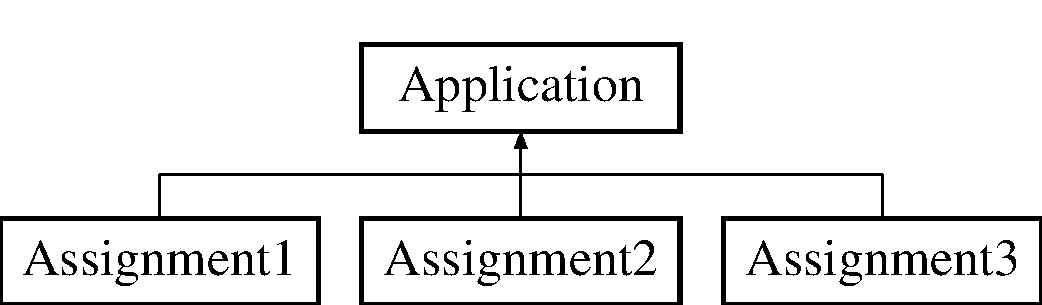
\includegraphics[height=2.000000cm]{class_application}
\end{center}
\end{figure}
\subsection*{Public Member Functions}
\begin{DoxyCompactItemize}
\item 
\hyperlink{class_application_a78cdcb03e6f06272f7c528fe407951c5}{Application} (std\+::shared\+\_\+ptr$<$ class \hyperlink{class_scene}{Scene} $>$ input\+Scene, std\+::shared\+\_\+ptr$<$ class \hyperlink{class_camera}{Camera} $>$ input\+Camera)
\begin{DoxyCompactList}\small\item\em Create an application with a pre-\/allocated scene and camera. \end{DoxyCompactList}\item 
\hypertarget{class_application_a748bca84fefb9c12661cfaa2f623748d}{}virtual \hyperlink{class_application_a748bca84fefb9c12661cfaa2f623748d}{$\sim$\+Application} ()\label{class_application_a748bca84fefb9c12661cfaa2f623748d}

\begin{DoxyCompactList}\small\item\em Virtual deconstrcutor to allow inheritance. \end{DoxyCompactList}\item 
virtual void \hyperlink{class_application_a17cf1ea4552d26a1c20f7d98d793d41d}{Initialize} ()
\begin{DoxyCompactList}\small\item\em Initialization function to setup the stored camera and scene. \end{DoxyCompactList}\item 
virtual std\+::unique\+\_\+ptr$<$ class \hyperlink{class_renderer}{Renderer} $>$ \hyperlink{class_application_a90c7fd9ecb6c8923948078903d442919}{Create\+Renderer} ()
\begin{DoxyCompactList}\small\item\em Creates a shared pointer of type \hyperlink{class_renderer}{Renderer}. \end{DoxyCompactList}\item 
virtual glm\+::vec2 \hyperlink{class_application_a3e9992f0ceae0d8beda7debccdb00534}{Get\+Window\+Size} () const 
\begin{DoxyCompactList}\small\item\em Specifies the initial window size. \end{DoxyCompactList}\item 
virtual bool \hyperlink{class_application_ae0019f2c58008791971e67f23f2d4182}{Is\+Finished} () const 
\begin{DoxyCompactList}\small\item\em Whether or not the application is finished running. \end{DoxyCompactList}\item 
virtual void \hyperlink{class_application_a9cbe96f94653eae2bb6ad5857b00fa10}{Request\+Exit} ()
\begin{DoxyCompactList}\small\item\em Notifies the \hyperlink{class_application}{Application} that it should finish. \end{DoxyCompactList}\item 
virtual void \hyperlink{class_application_a0800afd5651153d31fa775a8048d14dd}{Tick} (double delta\+Time)
\begin{DoxyCompactList}\small\item\em Called every frame to advance program logic. \end{DoxyCompactList}\item 
virtual void \hyperlink{class_application_afe6553c2828e6eb38f74af8d3a5a9c2f}{Handle\+Input} (S\+D\+L\+\_\+\+Keysym key, Uint32 state, Uint8 repeat, double timestamp)
\begin{DoxyCompactList}\small\item\em Processes an S\+D\+L keyboard event. Details about an S\+D\+L Keyboard event can be found \href{https://wiki.libsdl.org/SDL_KeyboardEvent}{\tt here} \end{DoxyCompactList}\item 
virtual void \hyperlink{class_application_a74d92db64e051efa56d0357989dcb755}{Handle\+Window\+Event} (S\+D\+L\+\_\+\+Window\+Event\+I\+D event\+Id, Sint32 data1, Sint32 data2, double timestamp)
\begin{DoxyCompactList}\small\item\em Processes an S\+D\+L window event. Details about an S\+D\+L window event can be found \href{https://wiki.libsdl.org/SDL_WindowEvent}{\tt here} \end{DoxyCompactList}\end{DoxyCompactItemize}
\subsection*{Static Public Member Functions}
\begin{DoxyCompactItemize}
\item 
static std\+::unique\+\_\+ptr$<$ \hyperlink{class_application}{Application} $>$ \hyperlink{class_application_a727f63f898a68bddf6d88309195ef194}{Create\+Application} (std\+::shared\+\_\+ptr$<$ class \hyperlink{class_scene}{Scene} $>$ scene, std\+::shared\+\_\+ptr$<$ class \hyperlink{class_camera}{Camera} $>$ camera)
\begin{DoxyCompactList}\small\item\em Creates a unique pointer to an \hyperlink{class_application}{Application}. This should be used instead of the constructor. \end{DoxyCompactList}\item 
static std\+::shared\+\_\+ptr$<$ class \hyperlink{class_scene}{Scene} $>$ \hyperlink{class_application_a511e638cf5748e10151f17d6140b9119}{Create\+Scene} ()
\begin{DoxyCompactList}\small\item\em Creates a shared pointer of type \hyperlink{class_scene}{Scene}. \end{DoxyCompactList}\item 
static std\+::shared\+\_\+ptr$<$ class \hyperlink{class_camera}{Camera} $>$ \hyperlink{class_application_a53c0a539fd2c4fe2cc48143cc0a3ea24}{Create\+Camera} ()
\begin{DoxyCompactList}\small\item\em Creates a shared pointer of type \hyperlink{class_camera}{Camera}. \end{DoxyCompactList}\end{DoxyCompactItemize}
\subsection*{Protected Member Functions}
\begin{DoxyCompactItemize}
\item 
\hypertarget{class_application_abdba284a0f075ee1d4a2108c3a5236a2}{}virtual void {\bfseries Handle\+Window\+Resize} (float x, float y)\label{class_application_abdba284a0f075ee1d4a2108c3a5236a2}

\end{DoxyCompactItemize}
\subsection*{Protected Attributes}
\begin{DoxyCompactItemize}
\item 
\hypertarget{class_application_ae1c1ff7a7663d9baa9b65a7ba8e1dcf8}{}bool {\bfseries is\+Running}\label{class_application_ae1c1ff7a7663d9baa9b65a7ba8e1dcf8}

\item 
\hypertarget{class_application_a88c6615107a5094bb93fa5f153f79554}{}std\+::shared\+\_\+ptr$<$ class \hyperlink{class_scene}{Scene} $>$ {\bfseries scene}\label{class_application_a88c6615107a5094bb93fa5f153f79554}

\item 
\hypertarget{class_application_a0e8589fcb13c520ba472473abe5a518d}{}std\+::shared\+\_\+ptr$<$ class \hyperlink{class_camera}{Camera} $>$ {\bfseries camera}\label{class_application_a0e8589fcb13c520ba472473abe5a518d}

\end{DoxyCompactItemize}


\subsection{Detailed Description}
Handles creating configurable objects (i.\+e. scene, camera, renderer), handling S\+D\+L events passed in by the \hyperlink{class_media_layer}{Media\+Layer}, and handles creating the scene to be display. 

An \textquotesingle{}\hyperlink{class_application}{Application}\textquotesingle{} M\+U\+S\+T be created to run the assignment framework. By default, the application will create a 1280x720 window that is completely black. After the \textquotesingle{}\hyperlink{class_application}{Application}\textquotesingle{} is created, it must be passed to the \textquotesingle{}\hyperlink{class_media_layer}{Media\+Layer}\textquotesingle{} who will call the \textquotesingle{}\hyperlink{class_application}{Application}\textquotesingle{}s tick function every frame. 

Definition at line 14 of file Application.\+h.



\subsection{Constructor \& Destructor Documentation}
\hypertarget{class_application_a78cdcb03e6f06272f7c528fe407951c5}{}\index{Application@{Application}!Application@{Application}}
\index{Application@{Application}!Application@{Application}}
\subsubsection[{Application}]{\setlength{\rightskip}{0pt plus 5cm}Application\+::\+Application (
\begin{DoxyParamCaption}
\item[{std\+::shared\+\_\+ptr$<$ class {\bf Scene} $>$}]{input\+Scene, }
\item[{std\+::shared\+\_\+ptr$<$ class {\bf Camera} $>$}]{input\+Camera}
\end{DoxyParamCaption}
)}\label{class_application_a78cdcb03e6f06272f7c528fe407951c5}


Create an application with a pre-\/allocated scene and camera. 


\begin{DoxyParams}{Parameters}
{\em input\+Scene} & A pre-\/allocated scene. This should be generated using \hyperlink{class_application_a511e638cf5748e10151f17d6140b9119}{Create\+Scene()} in the appropriate subclass. \\
\hline
{\em input\+Camera} & A pre-\/allocated camera. This should be generated using \hyperlink{class_application_a53c0a539fd2c4fe2cc48143cc0a3ea24}{Create\+Camera()} in the appropriate subclass. \\
\hline
\end{DoxyParams}
\begin{DoxyWarning}{Warning}
Do not use directly. Use Create\+Application instead. 
\end{DoxyWarning}


Definition at line 6 of file Application.\+cpp.



\subsection{Member Function Documentation}
\hypertarget{class_application_a727f63f898a68bddf6d88309195ef194}{}\index{Application@{Application}!Create\+Application@{Create\+Application}}
\index{Create\+Application@{Create\+Application}!Application@{Application}}
\subsubsection[{Create\+Application}]{\setlength{\rightskip}{0pt plus 5cm}std\+::unique\+\_\+ptr$<$ {\bf Application} $>$ Application\+::\+Create\+Application (
\begin{DoxyParamCaption}
\item[{std\+::shared\+\_\+ptr$<$ class {\bf Scene} $>$}]{scene, }
\item[{std\+::shared\+\_\+ptr$<$ class {\bf Camera} $>$}]{camera}
\end{DoxyParamCaption}
)\hspace{0.3cm}{\ttfamily [static]}}\label{class_application_a727f63f898a68bddf6d88309195ef194}


Creates a unique pointer to an \hyperlink{class_application}{Application}. This should be used instead of the constructor. 

\begin{DoxyReturn}{Returns}
A unique pointer to an \hyperlink{class_application}{Application}.
\end{DoxyReturn}
See \hyperlink{class_application_a78cdcb03e6f06272f7c528fe407951c5}{Application()} for more details. 

Definition at line 21 of file Application.\+cpp.

\hypertarget{class_application_a53c0a539fd2c4fe2cc48143cc0a3ea24}{}\index{Application@{Application}!Create\+Camera@{Create\+Camera}}
\index{Create\+Camera@{Create\+Camera}!Application@{Application}}
\subsubsection[{Create\+Camera}]{\setlength{\rightskip}{0pt plus 5cm}std\+::shared\+\_\+ptr$<$ {\bf Camera} $>$ Application\+::\+Create\+Camera (
\begin{DoxyParamCaption}
{}
\end{DoxyParamCaption}
)\hspace{0.3cm}{\ttfamily [static]}}\label{class_application_a53c0a539fd2c4fe2cc48143cc0a3ea24}


Creates a shared pointer of type \hyperlink{class_camera}{Camera}. 

\begin{DoxyReturn}{Returns}
A shared pointer to a \hyperlink{class_camera}{Camera}.
\end{DoxyReturn}
The subclass should also create a function \hyperlink{class_application_a53c0a539fd2c4fe2cc48143cc0a3ea24}{Create\+Camera()} that returns the proper type of \hyperlink{class_camera}{Camera} to create. 

Definition at line 31 of file Application.\+cpp.

\hypertarget{class_application_a90c7fd9ecb6c8923948078903d442919}{}\index{Application@{Application}!Create\+Renderer@{Create\+Renderer}}
\index{Create\+Renderer@{Create\+Renderer}!Application@{Application}}
\subsubsection[{Create\+Renderer}]{\setlength{\rightskip}{0pt plus 5cm}std\+::unique\+\_\+ptr$<$ class {\bf Renderer} $>$ Application\+::\+Create\+Renderer (
\begin{DoxyParamCaption}
{}
\end{DoxyParamCaption}
)\hspace{0.3cm}{\ttfamily [virtual]}}\label{class_application_a90c7fd9ecb6c8923948078903d442919}


Creates a shared pointer of type \hyperlink{class_renderer}{Renderer}. 

\begin{DoxyReturn}{Returns}
A unique pointer to a \hyperlink{class_renderer}{Renderer}.
\end{DoxyReturn}
The subclass should override this function \hyperlink{class_application_a90c7fd9ecb6c8923948078903d442919}{Create\+Renderer()} to return the proper type of \hyperlink{class_renderer}{Renderer} to create. 

Definition at line 36 of file Application.\+cpp.

\hypertarget{class_application_a511e638cf5748e10151f17d6140b9119}{}\index{Application@{Application}!Create\+Scene@{Create\+Scene}}
\index{Create\+Scene@{Create\+Scene}!Application@{Application}}
\subsubsection[{Create\+Scene}]{\setlength{\rightskip}{0pt plus 5cm}std\+::shared\+\_\+ptr$<$ {\bf Scene} $>$ Application\+::\+Create\+Scene (
\begin{DoxyParamCaption}
{}
\end{DoxyParamCaption}
)\hspace{0.3cm}{\ttfamily [static]}}\label{class_application_a511e638cf5748e10151f17d6140b9119}


Creates a shared pointer of type \hyperlink{class_scene}{Scene}. 

\begin{DoxyReturn}{Returns}
A shared pointer to a \hyperlink{class_scene}{Scene}.
\end{DoxyReturn}
The subclass should also create a function \hyperlink{class_application_a511e638cf5748e10151f17d6140b9119}{Create\+Scene()} that returns the proper type of \hyperlink{class_scene}{Scene} to create. 

Definition at line 26 of file Application.\+cpp.

\hypertarget{class_application_a3e9992f0ceae0d8beda7debccdb00534}{}\index{Application@{Application}!Get\+Window\+Size@{Get\+Window\+Size}}
\index{Get\+Window\+Size@{Get\+Window\+Size}!Application@{Application}}
\subsubsection[{Get\+Window\+Size}]{\setlength{\rightskip}{0pt plus 5cm}glm\+::vec2 Application\+::\+Get\+Window\+Size (
\begin{DoxyParamCaption}
{}
\end{DoxyParamCaption}
) const\hspace{0.3cm}{\ttfamily [virtual]}}\label{class_application_a3e9992f0ceae0d8beda7debccdb00534}


Specifies the initial window size. 

\begin{DoxyReturn}{Returns}
The desired window size. 
\end{DoxyReturn}


Reimplemented in \hyperlink{class_assignment2_ae7ae8c9e7eb64cf9661d9ddb1992f314}{Assignment2}, \hyperlink{class_assignment3_a895e38d50717c935706a719f4368f5e8}{Assignment3}, and \hyperlink{class_assignment1_a27daa24c1afe9e10bd6615dfa250473e}{Assignment1}.



Definition at line 41 of file Application.\+cpp.

\hypertarget{class_application_afe6553c2828e6eb38f74af8d3a5a9c2f}{}\index{Application@{Application}!Handle\+Input@{Handle\+Input}}
\index{Handle\+Input@{Handle\+Input}!Application@{Application}}
\subsubsection[{Handle\+Input}]{\setlength{\rightskip}{0pt plus 5cm}void Application\+::\+Handle\+Input (
\begin{DoxyParamCaption}
\item[{S\+D\+L\+\_\+\+Keysym}]{key, }
\item[{Uint32}]{state, }
\item[{Uint8}]{repeat, }
\item[{double}]{timestamp}
\end{DoxyParamCaption}
)\hspace{0.3cm}{\ttfamily [virtual]}}\label{class_application_afe6553c2828e6eb38f74af8d3a5a9c2f}


Processes an S\+D\+L keyboard event. Details about an S\+D\+L Keyboard event can be found \href{https://wiki.libsdl.org/SDL_KeyboardEvent}{\tt here} 


\begin{DoxyParams}{Parameters}
{\em key} & See the S\+D\+L documentation for more details about S\+D\+L\+\_\+\+Keysym. \href{https://wiki.libsdl.org/SDL_Keysym}{\tt Here} \\
\hline
{\em state} & This is the type field in the S\+D\+L\+\_\+\+Event datastructure. S\+D\+L Documentation\+: \href{https://wiki.libsdl.org/SDL_Event}{\tt Here} \\
\hline
{\em repeat} & This value is non-\/zero is the key is being repeated. \\
\hline
{\em timestamp} & Timestamp is the number of seconds since the program was first started.\\
\hline
\end{DoxyParams}
Although you get an input immediately, if you want to make a change to the scene, it is highly recommended that you queue a change and then process it within the \hyperlink{class_application_a0800afd5651153d31fa775a8048d14dd}{Tick()} function. This allows you to multiply by the appropriate delta when making a change. For example, an object moves at 10 meters per second and you want it to move forward when you hit the \textquotesingle{}W\textquotesingle{} key. How many units do you move forward by? You would move forward by $10 \cdot deltaTime$ 

Reimplemented in \hyperlink{class_assignment2_aca261dbf5bd583ecf013dccbe2abaf90}{Assignment2}, \hyperlink{class_assignment3_a7a3563e16c7fbd71d709decd266f6e9a}{Assignment3}, and \hyperlink{class_assignment1_a29da6ab20003bfec87bcc93474dc8ade}{Assignment1}.



Definition at line 70 of file Application.\+cpp.

\hypertarget{class_application_a74d92db64e051efa56d0357989dcb755}{}\index{Application@{Application}!Handle\+Window\+Event@{Handle\+Window\+Event}}
\index{Handle\+Window\+Event@{Handle\+Window\+Event}!Application@{Application}}
\subsubsection[{Handle\+Window\+Event}]{\setlength{\rightskip}{0pt plus 5cm}void Application\+::\+Handle\+Window\+Event (
\begin{DoxyParamCaption}
\item[{S\+D\+L\+\_\+\+Window\+Event\+I\+D}]{event\+Id, }
\item[{Sint32}]{data1, }
\item[{Sint32}]{data2, }
\item[{double}]{timestamp}
\end{DoxyParamCaption}
)\hspace{0.3cm}{\ttfamily [virtual]}}\label{class_application_a74d92db64e051efa56d0357989dcb755}


Processes an S\+D\+L window event. Details about an S\+D\+L window event can be found \href{https://wiki.libsdl.org/SDL_WindowEvent}{\tt here} 


\begin{DoxyParams}{Parameters}
{\em event\+Id} & This is an \href{https://wiki.libsdl.org/SDL_WindowEventID}{\tt S\+D\+L\+\_\+\+Window\+Event\+I\+D}. See the S\+D\+L documentation for more details. \\
\hline
{\em data1} & This changes depending on what event\+Id is. See the docs for S\+D\+L\+\_\+\+Window\+Event\+I\+D. \\
\hline
{\em data2} & This changes depending on what event\+Id is. See the docs for S\+D\+L\+\_\+\+Window\+Event\+I\+D. \\
\hline
{\em timestamp} & Timestamp is the number of seconds since the program was first started.\\
\hline
\end{DoxyParams}
This takes in a window event and process it. By default it handles when the size of the window changes and calls \href{https://www.opengl.org/sdk/docs/man/html/glViewport.xhtml}{\tt gl\+Viewport} to resize the viewport as necessary. You can expand on this functionality in the sub-\/class to handle other events such as the window moving, etc. However, make sure you maintain a call to \hyperlink{class_application_a74d92db64e051efa56d0357989dcb755}{Application\+::\+Handle\+Window\+Event()} to make sure gl\+Viewport is still called! 

Definition at line 74 of file Application.\+cpp.

\hypertarget{class_application_a17cf1ea4552d26a1c20f7d98d793d41d}{}\index{Application@{Application}!Initialize@{Initialize}}
\index{Initialize@{Initialize}!Application@{Application}}
\subsubsection[{Initialize}]{\setlength{\rightskip}{0pt plus 5cm}void Application\+::\+Initialize (
\begin{DoxyParamCaption}
{}
\end{DoxyParamCaption}
)\hspace{0.3cm}{\ttfamily [virtual]}}\label{class_application_a17cf1ea4552d26a1c20f7d98d793d41d}


Initialization function to setup the stored camera and scene. 

This initialization function exists because the Setup\+Scene() and Setup\+Camera() functions are virtual and thus can not exist within the constructor. This function is called in Media\+Layer\+::\+Media\+Layer(). 

Definition at line 15 of file Application.\+cpp.

\hypertarget{class_application_ae0019f2c58008791971e67f23f2d4182}{}\index{Application@{Application}!Is\+Finished@{Is\+Finished}}
\index{Is\+Finished@{Is\+Finished}!Application@{Application}}
\subsubsection[{Is\+Finished}]{\setlength{\rightskip}{0pt plus 5cm}bool Application\+::\+Is\+Finished (
\begin{DoxyParamCaption}
{}
\end{DoxyParamCaption}
) const\hspace{0.3cm}{\ttfamily [virtual]}}\label{class_application_ae0019f2c58008791971e67f23f2d4182}


Whether or not the application is finished running. 

\begin{DoxyReturn}{Returns}
Whether the application is finished running.
\end{DoxyReturn}
When the Media\+Layer\+::\+Tick() function detects that the application is finished, the program will exit. 

Definition at line 54 of file Application.\+cpp.

\hypertarget{class_application_a9cbe96f94653eae2bb6ad5857b00fa10}{}\index{Application@{Application}!Request\+Exit@{Request\+Exit}}
\index{Request\+Exit@{Request\+Exit}!Application@{Application}}
\subsubsection[{Request\+Exit}]{\setlength{\rightskip}{0pt plus 5cm}void Application\+::\+Request\+Exit (
\begin{DoxyParamCaption}
{}
\end{DoxyParamCaption}
)\hspace{0.3cm}{\ttfamily [virtual]}}\label{class_application_a9cbe96f94653eae2bb6ad5857b00fa10}


Notifies the \hyperlink{class_application}{Application} that it should finish. 

An external source (i.\+e. the \hyperlink{class_media_layer}{Media\+Layer}) may request for the \hyperlink{class_application}{Application} to finish. This lets the \hyperlink{class_application}{Application} exit gracefully. The \hyperlink{class_application}{Application} can choose to ignore the request (thought that is not recommended). After this function is called, \hyperlink{class_application_ae0019f2c58008791971e67f23f2d4182}{Is\+Finished()} should return true. 

Definition at line 59 of file Application.\+cpp.

\hypertarget{class_application_a0800afd5651153d31fa775a8048d14dd}{}\index{Application@{Application}!Tick@{Tick}}
\index{Tick@{Tick}!Application@{Application}}
\subsubsection[{Tick}]{\setlength{\rightskip}{0pt plus 5cm}void Application\+::\+Tick (
\begin{DoxyParamCaption}
\item[{double}]{delta\+Time}
\end{DoxyParamCaption}
)\hspace{0.3cm}{\ttfamily [virtual]}}\label{class_application_a0800afd5651153d31fa775a8048d14dd}


Called every frame to advance program logic. 


\begin{DoxyParams}{Parameters}
{\em delta\+Time} & The amount of time (in seconds) since the last tick.\\
\hline
\end{DoxyParams}
If you need something in the \hyperlink{class_scene}{Scene} to change over time, this is where you should implement that logic. It is recommended that you make use of the delta\+Time variable to make things change smoothly! 

Reimplemented in \hyperlink{class_assignment2_a41544ad361dd798d5fae1ec3197fc66e}{Assignment2}, and \hyperlink{class_assignment3_a11256b6e7b38ab24baa92729cfb8ffe2}{Assignment3}.



Definition at line 64 of file Application.\+cpp.



The documentation for this class was generated from the following files\+:\begin{DoxyCompactItemize}
\item 
/\+Users/michaelbao/workspace/cs148opengl4/source/common/Application.\+h\item 
/\+Users/michaelbao/workspace/cs148opengl4/source/common/Application.\+cpp\end{DoxyCompactItemize}

\hypertarget{class_assignment1}{}\section{Assignment1 Class Reference}
\label{class_assignment1}\index{Assignment1@{Assignment1}}


{\ttfamily \#include $<$Assignment1.\+h$>$}

Inheritance diagram for Assignment1\+:\begin{figure}[H]
\begin{center}
\leavevmode
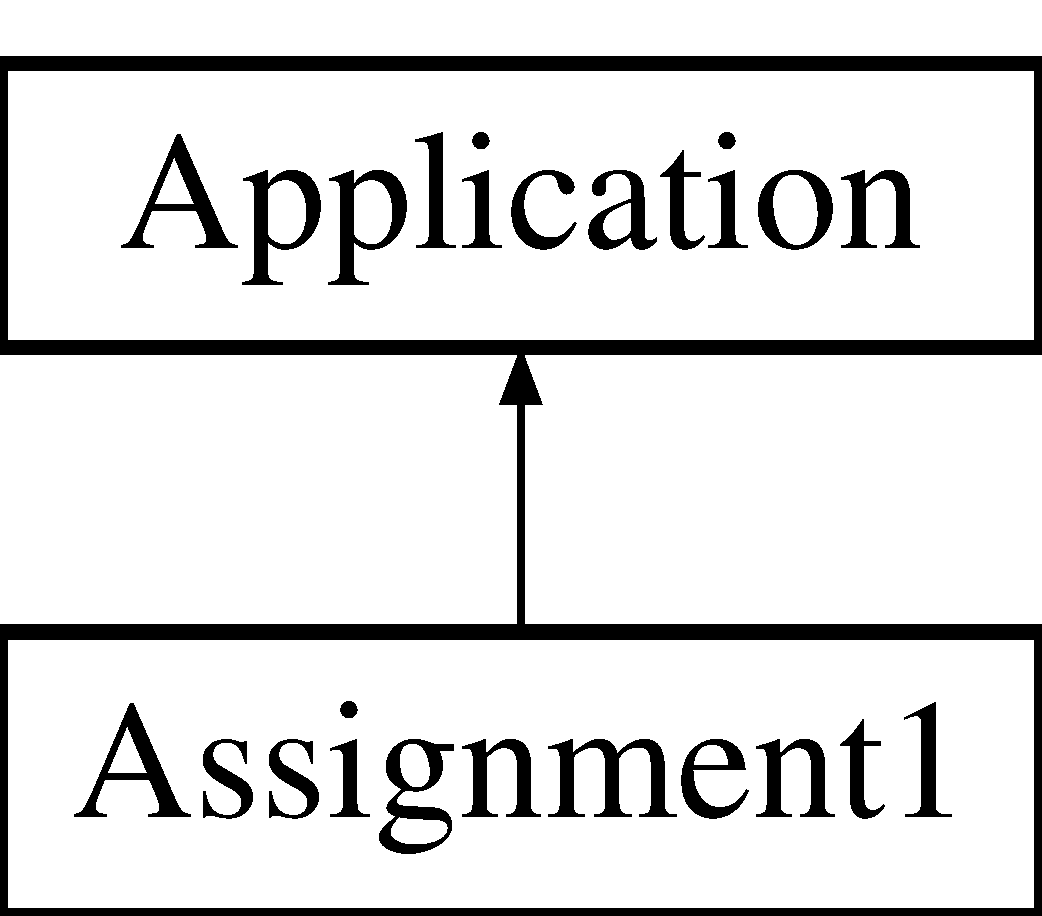
\includegraphics[height=2.000000cm]{class_assignment1}
\end{center}
\end{figure}
\subsection*{Public Member Functions}
\begin{DoxyCompactItemize}
\item 
\hyperlink{class_assignment1_ade9ef18c233dab37d37f20760fe7674d}{Assignment1} (std\+::shared\+\_\+ptr$<$ class \hyperlink{class_scene}{Scene} $>$ input\+Scene, std\+::shared\+\_\+ptr$<$ class \hyperlink{class_camera}{Camera} $>$ input\+Camera)
\item 
virtual glm\+::vec2 \hyperlink{class_assignment1_a27daa24c1afe9e10bd6615dfa250473e}{Get\+Window\+Size} () const 
\begin{DoxyCompactList}\small\item\em Specifies the initial window size. \end{DoxyCompactList}\item 
virtual void \hyperlink{class_assignment1_ab9db4f51e177dd72130cd61d86b97535}{Handle\+Input} (S\+D\+L\+\_\+\+Keysym key, Uint32 state, Uint8 repeat, double timestamp, double delta\+Time)
\begin{DoxyCompactList}\small\item\em Processes an S\+D\+L keyboard event which has type \href{https://wiki.libsdl.org/SDL_KeyboardEvent}{\tt S\+D\+L\+\_\+\+Keyboard\+Event}. \end{DoxyCompactList}\end{DoxyCompactItemize}
\subsection*{Static Public Member Functions}
\begin{DoxyCompactItemize}
\item 
static std\+::unique\+\_\+ptr$<$ \hyperlink{class_application}{Application} $>$ \hyperlink{class_assignment1_ae1952b4904620a16c4f2c098bf061c68}{Create\+Application} (std\+::shared\+\_\+ptr$<$ class \hyperlink{class_scene}{Scene} $>$ \hyperlink{class_application_a88c6615107a5094bb93fa5f153f79554}{scene}, std\+::shared\+\_\+ptr$<$ class \hyperlink{class_camera}{Camera} $>$ \hyperlink{class_application_a0e8589fcb13c520ba472473abe5a518d}{camera})
\end{DoxyCompactItemize}
\subsection*{Private Member Functions}
\begin{DoxyCompactItemize}
\item 
virtual void \hyperlink{class_assignment1_a8d12cf21f1463caa5a8da45110b50103}{Setup\+Scene} ()
\begin{DoxyCompactList}\small\item\em Called by \hyperlink{class_application_a17cf1ea4552d26a1c20f7d98d793d41d}{Initialize()} to populate the scene. \end{DoxyCompactList}\item 
virtual void \hyperlink{class_assignment1_a07743a6d86f7603dd58339c4db1de192}{Setup\+Example1} ()
\item 
virtual void \hyperlink{class_assignment1_aeabed7b579d59a6fdacaeab468afba29}{Setup\+Example2} ()
\item 
virtual void \hyperlink{class_assignment1_afbb3cb7765b899e69c9847d29f045392}{Setup\+Example3} ()
\end{DoxyCompactItemize}
\subsection*{Additional Inherited Members}


\subsection{Detailed Description}


Definition at line 8 of file Assignment1.\+h.



\subsection{Constructor \& Destructor Documentation}
\hypertarget{class_assignment1_ade9ef18c233dab37d37f20760fe7674d}{}\index{Assignment1@{Assignment1}!Assignment1@{Assignment1}}
\index{Assignment1@{Assignment1}!Assignment1@{Assignment1}}
\subsubsection[{Assignment1}]{\setlength{\rightskip}{0pt plus 5cm}Assignment1\+::\+Assignment1 (
\begin{DoxyParamCaption}
\item[{std\+::shared\+\_\+ptr$<$ class {\bf Scene} $>$}]{input\+Scene, }
\item[{std\+::shared\+\_\+ptr$<$ class {\bf Camera} $>$}]{input\+Camera}
\end{DoxyParamCaption}
)}\label{class_assignment1_ade9ef18c233dab37d37f20760fe7674d}


Definition at line 4 of file Assignment1.\+cpp.



\subsection{Member Function Documentation}
\hypertarget{class_assignment1_ae1952b4904620a16c4f2c098bf061c68}{}\index{Assignment1@{Assignment1}!Create\+Application@{Create\+Application}}
\index{Create\+Application@{Create\+Application}!Assignment1@{Assignment1}}
\subsubsection[{Create\+Application}]{\setlength{\rightskip}{0pt plus 5cm}std\+::unique\+\_\+ptr$<$ {\bf Application} $>$ Assignment1\+::\+Create\+Application (
\begin{DoxyParamCaption}
\item[{std\+::shared\+\_\+ptr$<$ class {\bf Scene} $>$}]{scene, }
\item[{std\+::shared\+\_\+ptr$<$ class {\bf Camera} $>$}]{camera}
\end{DoxyParamCaption}
)\hspace{0.3cm}{\ttfamily [static]}}\label{class_assignment1_ae1952b4904620a16c4f2c098bf061c68}


Definition at line 9 of file Assignment1.\+cpp.

\hypertarget{class_assignment1_a27daa24c1afe9e10bd6615dfa250473e}{}\index{Assignment1@{Assignment1}!Get\+Window\+Size@{Get\+Window\+Size}}
\index{Get\+Window\+Size@{Get\+Window\+Size}!Assignment1@{Assignment1}}
\subsubsection[{Get\+Window\+Size}]{\setlength{\rightskip}{0pt plus 5cm}glm\+::vec2 Assignment1\+::\+Get\+Window\+Size (
\begin{DoxyParamCaption}
{}
\end{DoxyParamCaption}
) const\hspace{0.3cm}{\ttfamily [virtual]}}\label{class_assignment1_a27daa24c1afe9e10bd6615dfa250473e}


Specifies the initial window size. 

\begin{DoxyReturn}{Returns}
The desired window size. 
\end{DoxyReturn}


Reimplemented from \hyperlink{class_application_a3e9992f0ceae0d8beda7debccdb00534}{Application}.



Definition at line 14 of file Assignment1.\+cpp.

\hypertarget{class_assignment1_ab9db4f51e177dd72130cd61d86b97535}{}\index{Assignment1@{Assignment1}!Handle\+Input@{Handle\+Input}}
\index{Handle\+Input@{Handle\+Input}!Assignment1@{Assignment1}}
\subsubsection[{Handle\+Input}]{\setlength{\rightskip}{0pt plus 5cm}void Assignment1\+::\+Handle\+Input (
\begin{DoxyParamCaption}
\item[{S\+D\+L\+\_\+\+Keysym}]{key, }
\item[{Uint32}]{state, }
\item[{Uint8}]{repeat, }
\item[{double}]{timestamp, }
\item[{double}]{delta\+Time}
\end{DoxyParamCaption}
)\hspace{0.3cm}{\ttfamily [virtual]}}\label{class_assignment1_ab9db4f51e177dd72130cd61d86b97535}


Processes an S\+D\+L keyboard event which has type \href{https://wiki.libsdl.org/SDL_KeyboardEvent}{\tt S\+D\+L\+\_\+\+Keyboard\+Event}. 


\begin{DoxyParams}{Parameters}
{\em key} & See the S\+D\+L documentation for more details about \href{https://wiki.libsdl.org/SDL_Keysym}{\tt S\+D\+L\+\_\+\+Keysym}. \\
\hline
{\em state} & This is the type field in the \href{https://wiki.libsdl.org/SDL_Event}{\tt S\+D\+L\+\_\+\+Event}datastructure. \\
\hline
{\em repeat} & This value is non-\/zero is the key is being repeated. \\
\hline
{\em timestamp} & Timestamp is the number of seconds since the program was first started. \\
\hline
{\em delta\+Time} & The amount of time (in seconds) since the last tick.\\
\hline
\end{DoxyParams}
Takes in a keyboard event and process it. This does nothing by default. \textquotesingle{}delta\+Time\textquotesingle{} is included to allow you to move something and have the movement look smooth. For example, if you have an object that you want to move forward whenever \textquotesingle{}W\textquotesingle{} is pressed. You know that the object travels at 10 meters per second when \textquotesingle{}W\textquotesingle{} is pressed and 0 meters per second when it is not. How far should you move the object? You would want to move it forward by $10 \cdot deltaTime $ units. 

Reimplemented from \hyperlink{class_application_ae6074c3f102de1cb2fe4c81b545679db}{Application}.



Definition at line 171 of file Assignment1.\+cpp.

\hypertarget{class_assignment1_a07743a6d86f7603dd58339c4db1de192}{}\index{Assignment1@{Assignment1}!Setup\+Example1@{Setup\+Example1}}
\index{Setup\+Example1@{Setup\+Example1}!Assignment1@{Assignment1}}
\subsubsection[{Setup\+Example1}]{\setlength{\rightskip}{0pt plus 5cm}void Assignment1\+::\+Setup\+Example1 (
\begin{DoxyParamCaption}
{}
\end{DoxyParamCaption}
)\hspace{0.3cm}{\ttfamily [private]}, {\ttfamily [virtual]}}\label{class_assignment1_a07743a6d86f7603dd58339c4db1de192}


Definition at line 24 of file Assignment1.\+cpp.

\hypertarget{class_assignment1_aeabed7b579d59a6fdacaeab468afba29}{}\index{Assignment1@{Assignment1}!Setup\+Example2@{Setup\+Example2}}
\index{Setup\+Example2@{Setup\+Example2}!Assignment1@{Assignment1}}
\subsubsection[{Setup\+Example2}]{\setlength{\rightskip}{0pt plus 5cm}void Assignment1\+::\+Setup\+Example2 (
\begin{DoxyParamCaption}
{}
\end{DoxyParamCaption}
)\hspace{0.3cm}{\ttfamily [private]}, {\ttfamily [virtual]}}\label{class_assignment1_aeabed7b579d59a6fdacaeab468afba29}


Definition at line 64 of file Assignment1.\+cpp.

\hypertarget{class_assignment1_afbb3cb7765b899e69c9847d29f045392}{}\index{Assignment1@{Assignment1}!Setup\+Example3@{Setup\+Example3}}
\index{Setup\+Example3@{Setup\+Example3}!Assignment1@{Assignment1}}
\subsubsection[{Setup\+Example3}]{\setlength{\rightskip}{0pt plus 5cm}void Assignment1\+::\+Setup\+Example3 (
\begin{DoxyParamCaption}
{}
\end{DoxyParamCaption}
)\hspace{0.3cm}{\ttfamily [private]}, {\ttfamily [virtual]}}\label{class_assignment1_afbb3cb7765b899e69c9847d29f045392}


Definition at line 106 of file Assignment1.\+cpp.

\hypertarget{class_assignment1_a8d12cf21f1463caa5a8da45110b50103}{}\index{Assignment1@{Assignment1}!Setup\+Scene@{Setup\+Scene}}
\index{Setup\+Scene@{Setup\+Scene}!Assignment1@{Assignment1}}
\subsubsection[{Setup\+Scene}]{\setlength{\rightskip}{0pt plus 5cm}void Assignment1\+::\+Setup\+Scene (
\begin{DoxyParamCaption}
{}
\end{DoxyParamCaption}
)\hspace{0.3cm}{\ttfamily [private]}, {\ttfamily [virtual]}}\label{class_assignment1_a8d12cf21f1463caa5a8da45110b50103}


Called by \hyperlink{class_application_a17cf1ea4552d26a1c20f7d98d793d41d}{Initialize()} to populate the scene. 

Note by the time this function is called, the \hyperlink{class_application}{Application} sub-\/class is fully constructed and \hyperlink{class_scene}{Scene} object is already created. 

Reimplemented from \hyperlink{class_application_aa8e8017ef8dd86293c96d0645e66d440}{Application}.



Definition at line 19 of file Assignment1.\+cpp.



The documentation for this class was generated from the following files\+:\begin{DoxyCompactItemize}
\item 
/\+Users/michaelbao/\+Phys\+B\+A\+M/\+Courses/2015/cs148/cs148opengl4/source/assignment1/\hyperlink{_assignment1_8h}{Assignment1.\+h}\item 
/\+Users/michaelbao/\+Phys\+B\+A\+M/\+Courses/2015/cs148/cs148opengl4/source/assignment1/\hyperlink{_assignment1_8cpp}{Assignment1.\+cpp}\end{DoxyCompactItemize}

\hypertarget{class_assignment2}{}\section{Assignment2 Class Reference}
\label{class_assignment2}\index{Assignment2@{Assignment2}}


{\ttfamily \#include $<$Assignment2.\+h$>$}

Inheritance diagram for Assignment2\+:\begin{figure}[H]
\begin{center}
\leavevmode
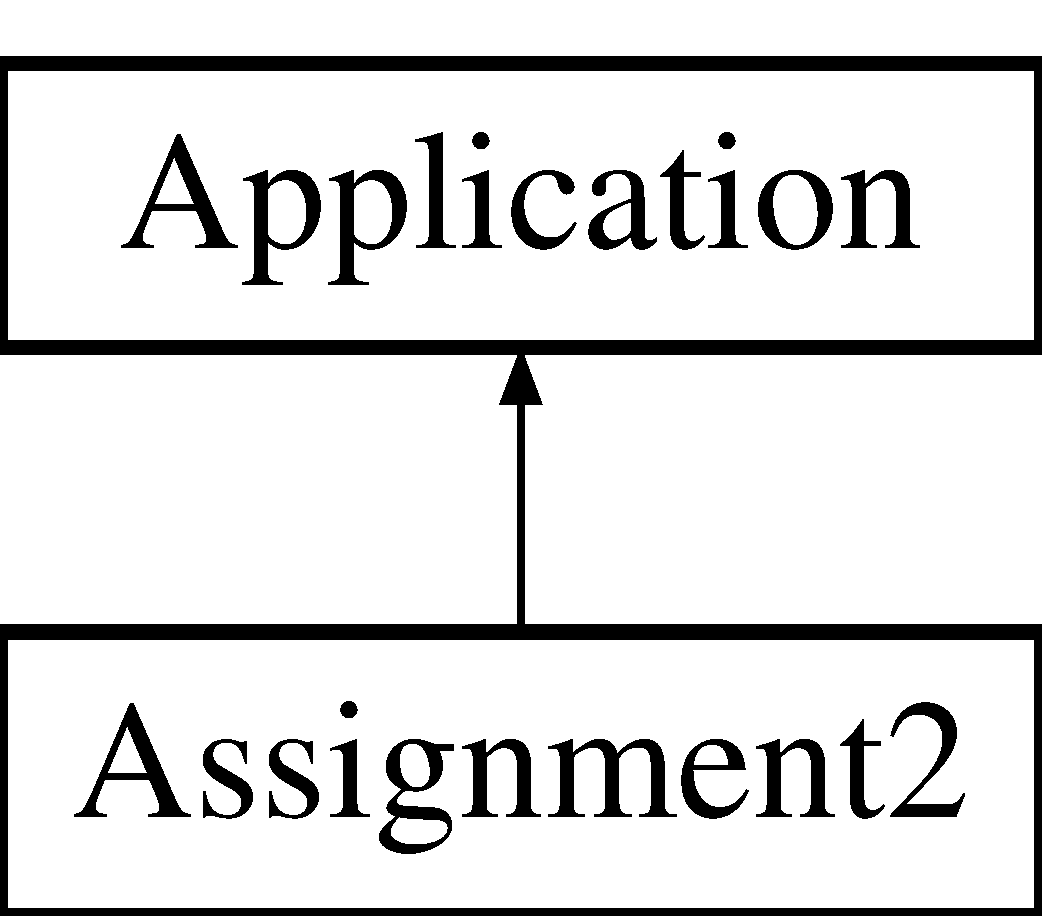
\includegraphics[height=2.000000cm]{class_assignment2}
\end{center}
\end{figure}
\subsection*{Public Member Functions}
\begin{DoxyCompactItemize}
\item 
\hyperlink{class_assignment2_ac684d2ecb894a4e71f8359e3a2ebd37f}{Assignment2} (std\+::shared\+\_\+ptr$<$ class \hyperlink{class_scene}{Scene} $>$ input\+Scene, std\+::shared\+\_\+ptr$<$ class \hyperlink{class_camera}{Camera} $>$ input\+Camera)
\item 
virtual glm\+::vec2 \hyperlink{class_assignment2_ae7ae8c9e7eb64cf9661d9ddb1992f314}{Get\+Window\+Size} () const 
\begin{DoxyCompactList}\small\item\em Specifies the initial window size. \end{DoxyCompactList}\item 
virtual void \hyperlink{class_assignment2_a3ee099a8ba45db14103541981e3c4fe8}{Handle\+Input} (S\+D\+L\+\_\+\+Keysym key, Uint32 state, Uint8 repeat, double timestamp, double delta\+Time)
\begin{DoxyCompactList}\small\item\em Processes an S\+D\+L keyboard event which has type \href{https://wiki.libsdl.org/SDL_KeyboardEvent}{\tt S\+D\+L\+\_\+\+Keyboard\+Event}. \end{DoxyCompactList}\item 
virtual void \hyperlink{class_assignment2_a41544ad361dd798d5fae1ec3197fc66e}{Tick} (double delta\+Time)
\begin{DoxyCompactList}\small\item\em Called every frame to advance program logic. \end{DoxyCompactList}\end{DoxyCompactItemize}
\subsection*{Static Public Member Functions}
\begin{DoxyCompactItemize}
\item 
static std\+::unique\+\_\+ptr$<$ \hyperlink{class_application}{Application} $>$ \hyperlink{class_assignment2_ae4f0035275d5be2c053a598fbe3209e6}{Create\+Application} (std\+::shared\+\_\+ptr$<$ class \hyperlink{class_scene}{Scene} $>$ \hyperlink{class_application_a88c6615107a5094bb93fa5f153f79554}{scene}, std\+::shared\+\_\+ptr$<$ class \hyperlink{class_camera}{Camera} $>$ \hyperlink{class_application_a0e8589fcb13c520ba472473abe5a518d}{camera})
\item 
static std\+::shared\+\_\+ptr$<$ class \hyperlink{class_camera}{Camera} $>$ \hyperlink{class_assignment2_a285e6d6ff330c03e28e49660ec178fa4}{Create\+Camera} ()
\end{DoxyCompactItemize}
\subsection*{Protected Member Functions}
\begin{DoxyCompactItemize}
\item 
virtual void \hyperlink{class_assignment2_a1af734567de5e8e73a2fd726fe3914f2}{Handle\+Window\+Resize} (float x, float y)
\begin{DoxyCompactList}\small\item\em Called by \hyperlink{class_application_a74d92db64e051efa56d0357989dcb755}{Handle\+Window\+Event()} when the window is resized. \end{DoxyCompactList}\end{DoxyCompactItemize}
\subsection*{Private Member Functions}
\begin{DoxyCompactItemize}
\item 
virtual void \hyperlink{class_assignment2_aa4f8ccd09a7accbdf093394c6ee4f63f}{Setup\+Scene} ()
\begin{DoxyCompactList}\small\item\em Called by \hyperlink{class_application_a17cf1ea4552d26a1c20f7d98d793d41d}{Initialize()} to populate the scene. \end{DoxyCompactList}\item 
virtual void \hyperlink{class_assignment2_a2f42c6da59d8b5ba5dc4796d8bd13d30}{Setup\+Example1} ()
\item 
virtual void \hyperlink{class_assignment2_aa26c3cd3e97be7ef88aae8d26d4af6bc}{Setup\+Example2} ()
\item 
virtual void \hyperlink{class_assignment2_a72e9b3939215d9a93bf5dc2090b35410}{Setup\+Example3} ()
\item 
virtual void \hyperlink{class_assignment2_ab9ace1ffdac8f7425c64d661f3d13acd}{Setup\+Camera} ()
\begin{DoxyCompactList}\small\item\em Called by \hyperlink{class_application_a17cf1ea4552d26a1c20f7d98d793d41d}{Initialize()} to setup the camera. \end{DoxyCompactList}\end{DoxyCompactItemize}
\subsection*{Private Attributes}
\begin{DoxyCompactItemize}
\item 
std\+::shared\+\_\+ptr$<$ class \hyperlink{class_scene_object}{Scene\+Object} $>$ \hyperlink{class_assignment2_a3afcc7cf71f0b1eb855482057beb1146}{scene\+Object}
\item 
std\+::shared\+\_\+ptr$<$ class \hyperlink{class_light}{Light} $>$ \hyperlink{class_assignment2_abaf6127e0de097717673c0d9b04f8c79}{point\+Light}
\item 
std\+::shared\+\_\+ptr$<$ class \hyperlink{class_light}{Light} $>$ \hyperlink{class_assignment2_adad4306da57243fada86a48e4edd7063}{point\+Light2}
\item 
std\+::shared\+\_\+ptr$<$ class \hyperlink{class_light}{Light} $>$ \hyperlink{class_assignment2_a23856ba0cbb408090482755bb636a567}{point\+Light3}
\item 
float \hyperlink{class_assignment2_a1406a4603687f934feca8cf72a850bd5}{elapsed\+Time}
\end{DoxyCompactItemize}
\subsection*{Additional Inherited Members}


\subsection{Detailed Description}


Definition at line 8 of file Assignment2.\+h.



\subsection{Constructor \& Destructor Documentation}
\hypertarget{class_assignment2_ac684d2ecb894a4e71f8359e3a2ebd37f}{}\index{Assignment2@{Assignment2}!Assignment2@{Assignment2}}
\index{Assignment2@{Assignment2}!Assignment2@{Assignment2}}
\subsubsection[{Assignment2}]{\setlength{\rightskip}{0pt plus 5cm}Assignment2\+::\+Assignment2 (
\begin{DoxyParamCaption}
\item[{std\+::shared\+\_\+ptr$<$ class {\bf Scene} $>$}]{input\+Scene, }
\item[{std\+::shared\+\_\+ptr$<$ class {\bf Camera} $>$}]{input\+Camera}
\end{DoxyParamCaption}
)}\label{class_assignment2_ac684d2ecb894a4e71f8359e3a2ebd37f}


Definition at line 7 of file Assignment2.\+cpp.



\subsection{Member Function Documentation}
\hypertarget{class_assignment2_ae4f0035275d5be2c053a598fbe3209e6}{}\index{Assignment2@{Assignment2}!Create\+Application@{Create\+Application}}
\index{Create\+Application@{Create\+Application}!Assignment2@{Assignment2}}
\subsubsection[{Create\+Application}]{\setlength{\rightskip}{0pt plus 5cm}std\+::unique\+\_\+ptr$<$ {\bf Application} $>$ Assignment2\+::\+Create\+Application (
\begin{DoxyParamCaption}
\item[{std\+::shared\+\_\+ptr$<$ class {\bf Scene} $>$}]{scene, }
\item[{std\+::shared\+\_\+ptr$<$ class {\bf Camera} $>$}]{camera}
\end{DoxyParamCaption}
)\hspace{0.3cm}{\ttfamily [static]}}\label{class_assignment2_ae4f0035275d5be2c053a598fbe3209e6}


Definition at line 12 of file Assignment2.\+cpp.

\hypertarget{class_assignment2_a285e6d6ff330c03e28e49660ec178fa4}{}\index{Assignment2@{Assignment2}!Create\+Camera@{Create\+Camera}}
\index{Create\+Camera@{Create\+Camera}!Assignment2@{Assignment2}}
\subsubsection[{Create\+Camera}]{\setlength{\rightskip}{0pt plus 5cm}std\+::shared\+\_\+ptr$<$ class {\bf Camera} $>$ Assignment2\+::\+Create\+Camera (
\begin{DoxyParamCaption}
{}
\end{DoxyParamCaption}
)\hspace{0.3cm}{\ttfamily [static]}}\label{class_assignment2_a285e6d6ff330c03e28e49660ec178fa4}


Definition at line 17 of file Assignment2.\+cpp.

\hypertarget{class_assignment2_ae7ae8c9e7eb64cf9661d9ddb1992f314}{}\index{Assignment2@{Assignment2}!Get\+Window\+Size@{Get\+Window\+Size}}
\index{Get\+Window\+Size@{Get\+Window\+Size}!Assignment2@{Assignment2}}
\subsubsection[{Get\+Window\+Size}]{\setlength{\rightskip}{0pt plus 5cm}glm\+::vec2 Assignment2\+::\+Get\+Window\+Size (
\begin{DoxyParamCaption}
{}
\end{DoxyParamCaption}
) const\hspace{0.3cm}{\ttfamily [virtual]}}\label{class_assignment2_ae7ae8c9e7eb64cf9661d9ddb1992f314}


Specifies the initial window size. 

\begin{DoxyReturn}{Returns}
The desired window size. 
\end{DoxyReturn}


Reimplemented from \hyperlink{class_application_a3e9992f0ceae0d8beda7debccdb00534}{Application}.



Definition at line 25 of file Assignment2.\+cpp.

\hypertarget{class_assignment2_a3ee099a8ba45db14103541981e3c4fe8}{}\index{Assignment2@{Assignment2}!Handle\+Input@{Handle\+Input}}
\index{Handle\+Input@{Handle\+Input}!Assignment2@{Assignment2}}
\subsubsection[{Handle\+Input}]{\setlength{\rightskip}{0pt plus 5cm}void Assignment2\+::\+Handle\+Input (
\begin{DoxyParamCaption}
\item[{S\+D\+L\+\_\+\+Keysym}]{key, }
\item[{Uint32}]{state, }
\item[{Uint8}]{repeat, }
\item[{double}]{timestamp, }
\item[{double}]{delta\+Time}
\end{DoxyParamCaption}
)\hspace{0.3cm}{\ttfamily [virtual]}}\label{class_assignment2_a3ee099a8ba45db14103541981e3c4fe8}


Processes an S\+D\+L keyboard event which has type \href{https://wiki.libsdl.org/SDL_KeyboardEvent}{\tt S\+D\+L\+\_\+\+Keyboard\+Event}. 


\begin{DoxyParams}{Parameters}
{\em key} & See the S\+D\+L documentation for more details about \href{https://wiki.libsdl.org/SDL_Keysym}{\tt S\+D\+L\+\_\+\+Keysym}. \\
\hline
{\em state} & This is the type field in the \href{https://wiki.libsdl.org/SDL_Event}{\tt S\+D\+L\+\_\+\+Event}datastructure. \\
\hline
{\em repeat} & This value is non-\/zero is the key is being repeated. \\
\hline
{\em timestamp} & Timestamp is the number of seconds since the program was first started. \\
\hline
{\em delta\+Time} & The amount of time (in seconds) since the last tick.\\
\hline
\end{DoxyParams}
Takes in a keyboard event and process it. This does nothing by default. \textquotesingle{}delta\+Time\textquotesingle{} is included to allow you to move something and have the movement look smooth. For example, if you have an object that you want to move forward whenever \textquotesingle{}W\textquotesingle{} is pressed. You know that the object travels at 10 meters per second when \textquotesingle{}W\textquotesingle{} is pressed and 0 meters per second when it is not. How far should you move the object? You would want to move it forward by $10 \cdot deltaTime $ units. 

Reimplemented from \hyperlink{class_application_ae6074c3f102de1cb2fe4c81b545679db}{Application}.



Definition at line 40 of file Assignment2.\+cpp.

\hypertarget{class_assignment2_a1af734567de5e8e73a2fd726fe3914f2}{}\index{Assignment2@{Assignment2}!Handle\+Window\+Resize@{Handle\+Window\+Resize}}
\index{Handle\+Window\+Resize@{Handle\+Window\+Resize}!Assignment2@{Assignment2}}
\subsubsection[{Handle\+Window\+Resize}]{\setlength{\rightskip}{0pt plus 5cm}void Assignment2\+::\+Handle\+Window\+Resize (
\begin{DoxyParamCaption}
\item[{float}]{x, }
\item[{float}]{y}
\end{DoxyParamCaption}
)\hspace{0.3cm}{\ttfamily [protected]}, {\ttfamily [virtual]}}\label{class_assignment2_a1af734567de5e8e73a2fd726fe3914f2}


Called by \hyperlink{class_application_a74d92db64e051efa56d0357989dcb755}{Handle\+Window\+Event()} when the window is resized. 


\begin{DoxyParams}{Parameters}
{\em x} & The width of the window. \\
\hline
{\em y} & The height of the window.\\
\hline
\end{DoxyParams}
By default calls, \href{https://www.opengl.org/sdk/docs/man/html/glViewport.xhtml}{\tt gl\+Viewport} to resize the viewport as necessary. If any part of your application depends on the window resize, you will want to take care of it in this function! (Hint for the O\+P\+T\+I\+O\+N\+A\+L deferred rendering task in assignment 2\+: your \textquotesingle{}G-\/\+Buffers\textquotesingle{} should be resized). 

Reimplemented from \hyperlink{class_application_abdba284a0f075ee1d4a2108c3a5236a2}{Application}.



Definition at line 105 of file Assignment2.\+cpp.

\hypertarget{class_assignment2_ab9ace1ffdac8f7425c64d661f3d13acd}{}\index{Assignment2@{Assignment2}!Setup\+Camera@{Setup\+Camera}}
\index{Setup\+Camera@{Setup\+Camera}!Assignment2@{Assignment2}}
\subsubsection[{Setup\+Camera}]{\setlength{\rightskip}{0pt plus 5cm}void Assignment2\+::\+Setup\+Camera (
\begin{DoxyParamCaption}
{}
\end{DoxyParamCaption}
)\hspace{0.3cm}{\ttfamily [private]}, {\ttfamily [virtual]}}\label{class_assignment2_ab9ace1ffdac8f7425c64d661f3d13acd}


Called by \hyperlink{class_application_a17cf1ea4552d26a1c20f7d98d793d41d}{Initialize()} to setup the camera. 

Note by the time this function is called, the \hyperlink{class_application}{Application} sub-\/class is fully constructed and \hyperlink{class_camera}{Camera} object is already created. 

Reimplemented from \hyperlink{class_application_a2eb61ca027f223a5c5ad1bf982481193}{Application}.



Definition at line 35 of file Assignment2.\+cpp.

\hypertarget{class_assignment2_a2f42c6da59d8b5ba5dc4796d8bd13d30}{}\index{Assignment2@{Assignment2}!Setup\+Example1@{Setup\+Example1}}
\index{Setup\+Example1@{Setup\+Example1}!Assignment2@{Assignment2}}
\subsubsection[{Setup\+Example1}]{\setlength{\rightskip}{0pt plus 5cm}void Assignment2\+::\+Setup\+Example1 (
\begin{DoxyParamCaption}
{}
\end{DoxyParamCaption}
)\hspace{0.3cm}{\ttfamily [private]}, {\ttfamily [virtual]}}\label{class_assignment2_a2f42c6da59d8b5ba5dc4796d8bd13d30}


Definition at line 111 of file Assignment2.\+cpp.

\hypertarget{class_assignment2_aa26c3cd3e97be7ef88aae8d26d4af6bc}{}\index{Assignment2@{Assignment2}!Setup\+Example2@{Setup\+Example2}}
\index{Setup\+Example2@{Setup\+Example2}!Assignment2@{Assignment2}}
\subsubsection[{Setup\+Example2}]{\setlength{\rightskip}{0pt plus 5cm}void Assignment2\+::\+Setup\+Example2 (
\begin{DoxyParamCaption}
{}
\end{DoxyParamCaption}
)\hspace{0.3cm}{\ttfamily [private]}, {\ttfamily [virtual]}}\label{class_assignment2_aa26c3cd3e97be7ef88aae8d26d4af6bc}


Definition at line 168 of file Assignment2.\+cpp.

\hypertarget{class_assignment2_a72e9b3939215d9a93bf5dc2090b35410}{}\index{Assignment2@{Assignment2}!Setup\+Example3@{Setup\+Example3}}
\index{Setup\+Example3@{Setup\+Example3}!Assignment2@{Assignment2}}
\subsubsection[{Setup\+Example3}]{\setlength{\rightskip}{0pt plus 5cm}void Assignment2\+::\+Setup\+Example3 (
\begin{DoxyParamCaption}
{}
\end{DoxyParamCaption}
)\hspace{0.3cm}{\ttfamily [private]}, {\ttfamily [virtual]}}\label{class_assignment2_a72e9b3939215d9a93bf5dc2090b35410}


Definition at line 224 of file Assignment2.\+cpp.

\hypertarget{class_assignment2_aa4f8ccd09a7accbdf093394c6ee4f63f}{}\index{Assignment2@{Assignment2}!Setup\+Scene@{Setup\+Scene}}
\index{Setup\+Scene@{Setup\+Scene}!Assignment2@{Assignment2}}
\subsubsection[{Setup\+Scene}]{\setlength{\rightskip}{0pt plus 5cm}void Assignment2\+::\+Setup\+Scene (
\begin{DoxyParamCaption}
{}
\end{DoxyParamCaption}
)\hspace{0.3cm}{\ttfamily [private]}, {\ttfamily [virtual]}}\label{class_assignment2_aa4f8ccd09a7accbdf093394c6ee4f63f}


Called by \hyperlink{class_application_a17cf1ea4552d26a1c20f7d98d793d41d}{Initialize()} to populate the scene. 

Note by the time this function is called, the \hyperlink{class_application}{Application} sub-\/class is fully constructed and \hyperlink{class_scene}{Scene} object is already created. 

Reimplemented from \hyperlink{class_application_aa8e8017ef8dd86293c96d0645e66d440}{Application}.



Definition at line 30 of file Assignment2.\+cpp.

\hypertarget{class_assignment2_a41544ad361dd798d5fae1ec3197fc66e}{}\index{Assignment2@{Assignment2}!Tick@{Tick}}
\index{Tick@{Tick}!Assignment2@{Assignment2}}
\subsubsection[{Tick}]{\setlength{\rightskip}{0pt plus 5cm}void Assignment2\+::\+Tick (
\begin{DoxyParamCaption}
\item[{double}]{delta\+Time}
\end{DoxyParamCaption}
)\hspace{0.3cm}{\ttfamily [virtual]}}\label{class_assignment2_a41544ad361dd798d5fae1ec3197fc66e}


Called every frame to advance program logic. 


\begin{DoxyParams}{Parameters}
{\em delta\+Time} & The amount of time (in seconds) since the last tick.\\
\hline
\end{DoxyParams}
If you need something in the \hyperlink{class_scene}{Scene} to change over time, this is where you should implement that logic. It is recommended that you make use of the delta\+Time variable to make things change smoothly! 

Reimplemented from \hyperlink{class_application_a0800afd5651153d31fa775a8048d14dd}{Application}.



Definition at line 273 of file Assignment2.\+cpp.



\subsection{Member Data Documentation}
\hypertarget{class_assignment2_a1406a4603687f934feca8cf72a850bd5}{}\index{Assignment2@{Assignment2}!elapsed\+Time@{elapsed\+Time}}
\index{elapsed\+Time@{elapsed\+Time}!Assignment2@{Assignment2}}
\subsubsection[{elapsed\+Time}]{\setlength{\rightskip}{0pt plus 5cm}float Assignment2\+::elapsed\+Time\hspace{0.3cm}{\ttfamily [private]}}\label{class_assignment2_a1406a4603687f934feca8cf72a850bd5}


Definition at line 37 of file Assignment2.\+h.

\hypertarget{class_assignment2_abaf6127e0de097717673c0d9b04f8c79}{}\index{Assignment2@{Assignment2}!point\+Light@{point\+Light}}
\index{point\+Light@{point\+Light}!Assignment2@{Assignment2}}
\subsubsection[{point\+Light}]{\setlength{\rightskip}{0pt plus 5cm}std\+::shared\+\_\+ptr$<$class {\bf Light}$>$ Assignment2\+::point\+Light\hspace{0.3cm}{\ttfamily [private]}}\label{class_assignment2_abaf6127e0de097717673c0d9b04f8c79}


Definition at line 34 of file Assignment2.\+h.

\hypertarget{class_assignment2_adad4306da57243fada86a48e4edd7063}{}\index{Assignment2@{Assignment2}!point\+Light2@{point\+Light2}}
\index{point\+Light2@{point\+Light2}!Assignment2@{Assignment2}}
\subsubsection[{point\+Light2}]{\setlength{\rightskip}{0pt plus 5cm}std\+::shared\+\_\+ptr$<$class {\bf Light}$>$ Assignment2\+::point\+Light2\hspace{0.3cm}{\ttfamily [private]}}\label{class_assignment2_adad4306da57243fada86a48e4edd7063}


Definition at line 35 of file Assignment2.\+h.

\hypertarget{class_assignment2_a23856ba0cbb408090482755bb636a567}{}\index{Assignment2@{Assignment2}!point\+Light3@{point\+Light3}}
\index{point\+Light3@{point\+Light3}!Assignment2@{Assignment2}}
\subsubsection[{point\+Light3}]{\setlength{\rightskip}{0pt plus 5cm}std\+::shared\+\_\+ptr$<$class {\bf Light}$>$ Assignment2\+::point\+Light3\hspace{0.3cm}{\ttfamily [private]}}\label{class_assignment2_a23856ba0cbb408090482755bb636a567}


Definition at line 36 of file Assignment2.\+h.

\hypertarget{class_assignment2_a3afcc7cf71f0b1eb855482057beb1146}{}\index{Assignment2@{Assignment2}!scene\+Object@{scene\+Object}}
\index{scene\+Object@{scene\+Object}!Assignment2@{Assignment2}}
\subsubsection[{scene\+Object}]{\setlength{\rightskip}{0pt plus 5cm}std\+::shared\+\_\+ptr$<$class {\bf Scene\+Object}$>$ Assignment2\+::scene\+Object\hspace{0.3cm}{\ttfamily [private]}}\label{class_assignment2_a3afcc7cf71f0b1eb855482057beb1146}


Definition at line 32 of file Assignment2.\+h.



The documentation for this class was generated from the following files\+:\begin{DoxyCompactItemize}
\item 
/\+Users/michaelbao/\+Phys\+B\+A\+M/\+Courses/2015/cs148/cs148opengl4/source/assignment2/\hyperlink{_assignment2_8h}{Assignment2.\+h}\item 
/\+Users/michaelbao/\+Phys\+B\+A\+M/\+Courses/2015/cs148/cs148opengl4/source/assignment2/\hyperlink{_assignment2_8cpp}{Assignment2.\+cpp}\end{DoxyCompactItemize}

\hypertarget{class_assignment3}{}\section{Assignment3 Class Reference}
\label{class_assignment3}\index{Assignment3@{Assignment3}}


{\ttfamily \#include $<$Assignment3.\+h$>$}

Inheritance diagram for Assignment3\+:\begin{figure}[H]
\begin{center}
\leavevmode
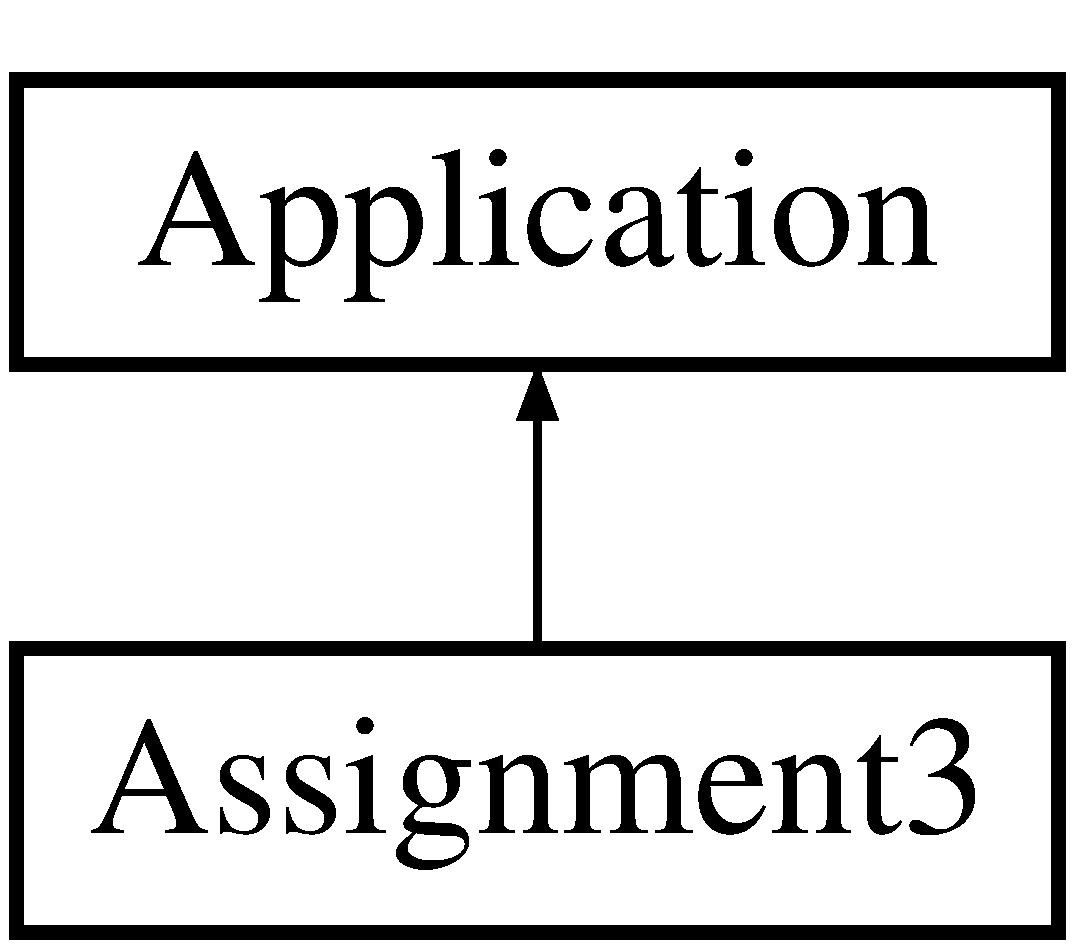
\includegraphics[height=2.000000cm]{class_assignment3}
\end{center}
\end{figure}
\subsection*{Public Member Functions}
\begin{DoxyCompactItemize}
\item 
\hyperlink{class_assignment3_adb8e9ac0681c600affc3370f5e5422b2}{Assignment3} (std\+::shared\+\_\+ptr$<$ class \hyperlink{class_scene}{Scene} $>$ input\+Scene, std\+::shared\+\_\+ptr$<$ class \hyperlink{class_camera}{Camera} $>$ input\+Camera)
\item 
virtual glm\+::vec2 \hyperlink{class_assignment3_a895e38d50717c935706a719f4368f5e8}{Get\+Window\+Size} () const 
\begin{DoxyCompactList}\small\item\em Specifies the initial window size. \end{DoxyCompactList}\item 
virtual void \hyperlink{class_assignment3_a1cc65ca321f39eb7092959b2dada8d31}{Handle\+Input} (S\+D\+L\+\_\+\+Keysym key, Uint32 state, Uint8 repeat, double timestamp, double delta\+Time)
\begin{DoxyCompactList}\small\item\em Processes an S\+D\+L keyboard event which has type \href{https://wiki.libsdl.org/SDL_KeyboardEvent}{\tt S\+D\+L\+\_\+\+Keyboard\+Event}. \end{DoxyCompactList}\item 
virtual void \hyperlink{class_assignment3_a11256b6e7b38ab24baa92729cfb8ffe2}{Tick} (double delta\+Time)
\begin{DoxyCompactList}\small\item\em Called every frame to advance program logic. \end{DoxyCompactList}\end{DoxyCompactItemize}
\subsection*{Static Public Member Functions}
\begin{DoxyCompactItemize}
\item 
static std\+::unique\+\_\+ptr$<$ \hyperlink{class_application}{Application} $>$ \hyperlink{class_assignment3_a12b30bd7b8a0bcefbd977f126ce00b25}{Create\+Application} (std\+::shared\+\_\+ptr$<$ class \hyperlink{class_scene}{Scene} $>$ \hyperlink{class_application_a88c6615107a5094bb93fa5f153f79554}{scene}, std\+::shared\+\_\+ptr$<$ class \hyperlink{class_camera}{Camera} $>$ \hyperlink{class_application_a0e8589fcb13c520ba472473abe5a518d}{camera})
\item 
static std\+::shared\+\_\+ptr$<$ class \hyperlink{class_camera}{Camera} $>$ \hyperlink{class_assignment3_a47d1b58079eee3e135e08768cd2a2461}{Create\+Camera} ()
\end{DoxyCompactItemize}
\subsection*{Protected Member Functions}
\begin{DoxyCompactItemize}
\item 
virtual void \hyperlink{class_assignment3_a851c637c83c8092d8adfb5c9f761daeb}{Handle\+Window\+Resize} (float x, float y)
\begin{DoxyCompactList}\small\item\em Called by \hyperlink{class_application_a74d92db64e051efa56d0357989dcb755}{Handle\+Window\+Event()} when the window is resized. \end{DoxyCompactList}\end{DoxyCompactItemize}
\subsection*{Private Member Functions}
\begin{DoxyCompactItemize}
\item 
virtual void \hyperlink{class_assignment3_a2dc29d9016a9d822ede84b9ef41429a5}{Setup\+Scene} ()
\begin{DoxyCompactList}\small\item\em Called by \hyperlink{class_application_a17cf1ea4552d26a1c20f7d98d793d41d}{Initialize()} to populate the scene. \end{DoxyCompactList}\item 
virtual void \hyperlink{class_assignment3_a468c30083d6f75d99cd1fe41205983dc}{Setup\+Example1} ()
\item 
virtual void \hyperlink{class_assignment3_a1d23eb19973b78e516169f4a03954526}{Setup\+Camera} ()
\begin{DoxyCompactList}\small\item\em Called by \hyperlink{class_application_a17cf1ea4552d26a1c20f7d98d793d41d}{Initialize()} to setup the camera. \end{DoxyCompactList}\end{DoxyCompactItemize}
\subsection*{Private Attributes}
\begin{DoxyCompactItemize}
\item 
std\+::shared\+\_\+ptr$<$ class \hyperlink{class_scene_object}{Scene\+Object} $>$ \hyperlink{class_assignment3_a0bc175d3efff30c5f4aa3ffa1272338a}{scene\+Object}
\item 
std\+::shared\+\_\+ptr$<$ class \hyperlink{class_light}{Light} $>$ \hyperlink{class_assignment3_ad1cf5a76d62b5a1ed17e66c31e0feb98}{point\+Light}
\item 
std\+::shared\+\_\+ptr$<$ class \hyperlink{class_light}{Light} $>$ \hyperlink{class_assignment3_ad6ea1201b058dbac9fd0e7b67015cf61}{point\+Light2}
\item 
std\+::shared\+\_\+ptr$<$ class \hyperlink{class_light}{Light} $>$ \hyperlink{class_assignment3_a59be58dbfebe4aa36097131bf654a7ae}{point\+Light3}
\item 
std\+::shared\+\_\+ptr$<$ class \hyperlink{class_light}{Light} $>$ \hyperlink{class_assignment3_af720bbd23f1f59d15908eb602a41725b}{point\+Light4}
\item 
float \hyperlink{class_assignment3_ac404a56071e2ab5e14289900b9034438}{elapsed\+Time}
\end{DoxyCompactItemize}
\subsection*{Additional Inherited Members}


\subsection{Detailed Description}


Definition at line 8 of file Assignment3.\+h.



\subsection{Constructor \& Destructor Documentation}
\hypertarget{class_assignment3_adb8e9ac0681c600affc3370f5e5422b2}{}\index{Assignment3@{Assignment3}!Assignment3@{Assignment3}}
\index{Assignment3@{Assignment3}!Assignment3@{Assignment3}}
\subsubsection[{Assignment3}]{\setlength{\rightskip}{0pt plus 5cm}Assignment3\+::\+Assignment3 (
\begin{DoxyParamCaption}
\item[{std\+::shared\+\_\+ptr$<$ class {\bf Scene} $>$}]{input\+Scene, }
\item[{std\+::shared\+\_\+ptr$<$ class {\bf Camera} $>$}]{input\+Camera}
\end{DoxyParamCaption}
)}\label{class_assignment3_adb8e9ac0681c600affc3370f5e5422b2}


Definition at line 8 of file Assignment3.\+cpp.



\subsection{Member Function Documentation}
\hypertarget{class_assignment3_a12b30bd7b8a0bcefbd977f126ce00b25}{}\index{Assignment3@{Assignment3}!Create\+Application@{Create\+Application}}
\index{Create\+Application@{Create\+Application}!Assignment3@{Assignment3}}
\subsubsection[{Create\+Application}]{\setlength{\rightskip}{0pt plus 5cm}std\+::unique\+\_\+ptr$<$ {\bf Application} $>$ Assignment3\+::\+Create\+Application (
\begin{DoxyParamCaption}
\item[{std\+::shared\+\_\+ptr$<$ class {\bf Scene} $>$}]{scene, }
\item[{std\+::shared\+\_\+ptr$<$ class {\bf Camera} $>$}]{camera}
\end{DoxyParamCaption}
)\hspace{0.3cm}{\ttfamily [static]}}\label{class_assignment3_a12b30bd7b8a0bcefbd977f126ce00b25}


Definition at line 13 of file Assignment3.\+cpp.

\hypertarget{class_assignment3_a47d1b58079eee3e135e08768cd2a2461}{}\index{Assignment3@{Assignment3}!Create\+Camera@{Create\+Camera}}
\index{Create\+Camera@{Create\+Camera}!Assignment3@{Assignment3}}
\subsubsection[{Create\+Camera}]{\setlength{\rightskip}{0pt plus 5cm}std\+::shared\+\_\+ptr$<$ class {\bf Camera} $>$ Assignment3\+::\+Create\+Camera (
\begin{DoxyParamCaption}
{}
\end{DoxyParamCaption}
)\hspace{0.3cm}{\ttfamily [static]}}\label{class_assignment3_a47d1b58079eee3e135e08768cd2a2461}


Definition at line 18 of file Assignment3.\+cpp.

\hypertarget{class_assignment3_a895e38d50717c935706a719f4368f5e8}{}\index{Assignment3@{Assignment3}!Get\+Window\+Size@{Get\+Window\+Size}}
\index{Get\+Window\+Size@{Get\+Window\+Size}!Assignment3@{Assignment3}}
\subsubsection[{Get\+Window\+Size}]{\setlength{\rightskip}{0pt plus 5cm}glm\+::vec2 Assignment3\+::\+Get\+Window\+Size (
\begin{DoxyParamCaption}
{}
\end{DoxyParamCaption}
) const\hspace{0.3cm}{\ttfamily [virtual]}}\label{class_assignment3_a895e38d50717c935706a719f4368f5e8}


Specifies the initial window size. 

\begin{DoxyReturn}{Returns}
The desired window size. 
\end{DoxyReturn}


Reimplemented from \hyperlink{class_application_a3e9992f0ceae0d8beda7debccdb00534}{Application}.



Definition at line 26 of file Assignment3.\+cpp.

\hypertarget{class_assignment3_a1cc65ca321f39eb7092959b2dada8d31}{}\index{Assignment3@{Assignment3}!Handle\+Input@{Handle\+Input}}
\index{Handle\+Input@{Handle\+Input}!Assignment3@{Assignment3}}
\subsubsection[{Handle\+Input}]{\setlength{\rightskip}{0pt plus 5cm}void Assignment3\+::\+Handle\+Input (
\begin{DoxyParamCaption}
\item[{S\+D\+L\+\_\+\+Keysym}]{key, }
\item[{Uint32}]{state, }
\item[{Uint8}]{repeat, }
\item[{double}]{timestamp, }
\item[{double}]{delta\+Time}
\end{DoxyParamCaption}
)\hspace{0.3cm}{\ttfamily [virtual]}}\label{class_assignment3_a1cc65ca321f39eb7092959b2dada8d31}


Processes an S\+D\+L keyboard event which has type \href{https://wiki.libsdl.org/SDL_KeyboardEvent}{\tt S\+D\+L\+\_\+\+Keyboard\+Event}. 


\begin{DoxyParams}{Parameters}
{\em key} & See the S\+D\+L documentation for more details about \href{https://wiki.libsdl.org/SDL_Keysym}{\tt S\+D\+L\+\_\+\+Keysym}. \\
\hline
{\em state} & This is the type field in the \href{https://wiki.libsdl.org/SDL_Event}{\tt S\+D\+L\+\_\+\+Event}datastructure. \\
\hline
{\em repeat} & This value is non-\/zero is the key is being repeated. \\
\hline
{\em timestamp} & Timestamp is the number of seconds since the program was first started. \\
\hline
{\em delta\+Time} & The amount of time (in seconds) since the last tick.\\
\hline
\end{DoxyParams}
Takes in a keyboard event and process it. This does nothing by default. \textquotesingle{}delta\+Time\textquotesingle{} is included to allow you to move something and have the movement look smooth. For example, if you have an object that you want to move forward whenever \textquotesingle{}W\textquotesingle{} is pressed. You know that the object travels at 10 meters per second when \textquotesingle{}W\textquotesingle{} is pressed and 0 meters per second when it is not. How far should you move the object? You would want to move it forward by $10 \cdot deltaTime $ units. 

Reimplemented from \hyperlink{class_application_ae6074c3f102de1cb2fe4c81b545679db}{Application}.



Definition at line 41 of file Assignment3.\+cpp.

\hypertarget{class_assignment3_a851c637c83c8092d8adfb5c9f761daeb}{}\index{Assignment3@{Assignment3}!Handle\+Window\+Resize@{Handle\+Window\+Resize}}
\index{Handle\+Window\+Resize@{Handle\+Window\+Resize}!Assignment3@{Assignment3}}
\subsubsection[{Handle\+Window\+Resize}]{\setlength{\rightskip}{0pt plus 5cm}void Assignment3\+::\+Handle\+Window\+Resize (
\begin{DoxyParamCaption}
\item[{float}]{x, }
\item[{float}]{y}
\end{DoxyParamCaption}
)\hspace{0.3cm}{\ttfamily [protected]}, {\ttfamily [virtual]}}\label{class_assignment3_a851c637c83c8092d8adfb5c9f761daeb}


Called by \hyperlink{class_application_a74d92db64e051efa56d0357989dcb755}{Handle\+Window\+Event()} when the window is resized. 


\begin{DoxyParams}{Parameters}
{\em x} & The width of the window. \\
\hline
{\em y} & The height of the window.\\
\hline
\end{DoxyParams}
By default calls, \href{https://www.opengl.org/sdk/docs/man/html/glViewport.xhtml}{\tt gl\+Viewport} to resize the viewport as necessary. If any part of your application depends on the window resize, you will want to take care of it in this function! (Hint for the O\+P\+T\+I\+O\+N\+A\+L deferred rendering task in assignment 2\+: your \textquotesingle{}G-\/\+Buffers\textquotesingle{} should be resized). 

Reimplemented from \hyperlink{class_application_abdba284a0f075ee1d4a2108c3a5236a2}{Application}.



Definition at line 96 of file Assignment3.\+cpp.

\hypertarget{class_assignment3_a1d23eb19973b78e516169f4a03954526}{}\index{Assignment3@{Assignment3}!Setup\+Camera@{Setup\+Camera}}
\index{Setup\+Camera@{Setup\+Camera}!Assignment3@{Assignment3}}
\subsubsection[{Setup\+Camera}]{\setlength{\rightskip}{0pt plus 5cm}void Assignment3\+::\+Setup\+Camera (
\begin{DoxyParamCaption}
{}
\end{DoxyParamCaption}
)\hspace{0.3cm}{\ttfamily [private]}, {\ttfamily [virtual]}}\label{class_assignment3_a1d23eb19973b78e516169f4a03954526}


Called by \hyperlink{class_application_a17cf1ea4552d26a1c20f7d98d793d41d}{Initialize()} to setup the camera. 

Note by the time this function is called, the \hyperlink{class_application}{Application} sub-\/class is fully constructed and \hyperlink{class_camera}{Camera} object is already created. 

Reimplemented from \hyperlink{class_application_a2eb61ca027f223a5c5ad1bf982481193}{Application}.



Definition at line 36 of file Assignment3.\+cpp.

\hypertarget{class_assignment3_a468c30083d6f75d99cd1fe41205983dc}{}\index{Assignment3@{Assignment3}!Setup\+Example1@{Setup\+Example1}}
\index{Setup\+Example1@{Setup\+Example1}!Assignment3@{Assignment3}}
\subsubsection[{Setup\+Example1}]{\setlength{\rightskip}{0pt plus 5cm}void Assignment3\+::\+Setup\+Example1 (
\begin{DoxyParamCaption}
{}
\end{DoxyParamCaption}
)\hspace{0.3cm}{\ttfamily [private]}, {\ttfamily [virtual]}}\label{class_assignment3_a468c30083d6f75d99cd1fe41205983dc}


Definition at line 102 of file Assignment3.\+cpp.

\hypertarget{class_assignment3_a2dc29d9016a9d822ede84b9ef41429a5}{}\index{Assignment3@{Assignment3}!Setup\+Scene@{Setup\+Scene}}
\index{Setup\+Scene@{Setup\+Scene}!Assignment3@{Assignment3}}
\subsubsection[{Setup\+Scene}]{\setlength{\rightskip}{0pt plus 5cm}void Assignment3\+::\+Setup\+Scene (
\begin{DoxyParamCaption}
{}
\end{DoxyParamCaption}
)\hspace{0.3cm}{\ttfamily [private]}, {\ttfamily [virtual]}}\label{class_assignment3_a2dc29d9016a9d822ede84b9ef41429a5}


Called by \hyperlink{class_application_a17cf1ea4552d26a1c20f7d98d793d41d}{Initialize()} to populate the scene. 

Note by the time this function is called, the \hyperlink{class_application}{Application} sub-\/class is fully constructed and \hyperlink{class_scene}{Scene} object is already created. 

Reimplemented from \hyperlink{class_application_aa8e8017ef8dd86293c96d0645e66d440}{Application}.



Definition at line 31 of file Assignment3.\+cpp.

\hypertarget{class_assignment3_a11256b6e7b38ab24baa92729cfb8ffe2}{}\index{Assignment3@{Assignment3}!Tick@{Tick}}
\index{Tick@{Tick}!Assignment3@{Assignment3}}
\subsubsection[{Tick}]{\setlength{\rightskip}{0pt plus 5cm}void Assignment3\+::\+Tick (
\begin{DoxyParamCaption}
\item[{double}]{delta\+Time}
\end{DoxyParamCaption}
)\hspace{0.3cm}{\ttfamily [virtual]}}\label{class_assignment3_a11256b6e7b38ab24baa92729cfb8ffe2}


Called every frame to advance program logic. 


\begin{DoxyParams}{Parameters}
{\em delta\+Time} & The amount of time (in seconds) since the last tick.\\
\hline
\end{DoxyParams}
If you need something in the \hyperlink{class_scene}{Scene} to change over time, this is where you should implement that logic. It is recommended that you make use of the delta\+Time variable to make things change smoothly! 

Reimplemented from \hyperlink{class_application_a0800afd5651153d31fa775a8048d14dd}{Application}.



Definition at line 179 of file Assignment3.\+cpp.



\subsection{Member Data Documentation}
\hypertarget{class_assignment3_ac404a56071e2ab5e14289900b9034438}{}\index{Assignment3@{Assignment3}!elapsed\+Time@{elapsed\+Time}}
\index{elapsed\+Time@{elapsed\+Time}!Assignment3@{Assignment3}}
\subsubsection[{elapsed\+Time}]{\setlength{\rightskip}{0pt plus 5cm}float Assignment3\+::elapsed\+Time\hspace{0.3cm}{\ttfamily [private]}}\label{class_assignment3_ac404a56071e2ab5e14289900b9034438}


Definition at line 35 of file Assignment3.\+h.

\hypertarget{class_assignment3_ad1cf5a76d62b5a1ed17e66c31e0feb98}{}\index{Assignment3@{Assignment3}!point\+Light@{point\+Light}}
\index{point\+Light@{point\+Light}!Assignment3@{Assignment3}}
\subsubsection[{point\+Light}]{\setlength{\rightskip}{0pt plus 5cm}std\+::shared\+\_\+ptr$<$class {\bf Light}$>$ Assignment3\+::point\+Light\hspace{0.3cm}{\ttfamily [private]}}\label{class_assignment3_ad1cf5a76d62b5a1ed17e66c31e0feb98}


Definition at line 31 of file Assignment3.\+h.

\hypertarget{class_assignment3_ad6ea1201b058dbac9fd0e7b67015cf61}{}\index{Assignment3@{Assignment3}!point\+Light2@{point\+Light2}}
\index{point\+Light2@{point\+Light2}!Assignment3@{Assignment3}}
\subsubsection[{point\+Light2}]{\setlength{\rightskip}{0pt plus 5cm}std\+::shared\+\_\+ptr$<$class {\bf Light}$>$ Assignment3\+::point\+Light2\hspace{0.3cm}{\ttfamily [private]}}\label{class_assignment3_ad6ea1201b058dbac9fd0e7b67015cf61}


Definition at line 32 of file Assignment3.\+h.

\hypertarget{class_assignment3_a59be58dbfebe4aa36097131bf654a7ae}{}\index{Assignment3@{Assignment3}!point\+Light3@{point\+Light3}}
\index{point\+Light3@{point\+Light3}!Assignment3@{Assignment3}}
\subsubsection[{point\+Light3}]{\setlength{\rightskip}{0pt plus 5cm}std\+::shared\+\_\+ptr$<$class {\bf Light}$>$ Assignment3\+::point\+Light3\hspace{0.3cm}{\ttfamily [private]}}\label{class_assignment3_a59be58dbfebe4aa36097131bf654a7ae}


Definition at line 33 of file Assignment3.\+h.

\hypertarget{class_assignment3_af720bbd23f1f59d15908eb602a41725b}{}\index{Assignment3@{Assignment3}!point\+Light4@{point\+Light4}}
\index{point\+Light4@{point\+Light4}!Assignment3@{Assignment3}}
\subsubsection[{point\+Light4}]{\setlength{\rightskip}{0pt plus 5cm}std\+::shared\+\_\+ptr$<$class {\bf Light}$>$ Assignment3\+::point\+Light4\hspace{0.3cm}{\ttfamily [private]}}\label{class_assignment3_af720bbd23f1f59d15908eb602a41725b}


Definition at line 34 of file Assignment3.\+h.

\hypertarget{class_assignment3_a0bc175d3efff30c5f4aa3ffa1272338a}{}\index{Assignment3@{Assignment3}!scene\+Object@{scene\+Object}}
\index{scene\+Object@{scene\+Object}!Assignment3@{Assignment3}}
\subsubsection[{scene\+Object}]{\setlength{\rightskip}{0pt plus 5cm}std\+::shared\+\_\+ptr$<$class {\bf Scene\+Object}$>$ Assignment3\+::scene\+Object\hspace{0.3cm}{\ttfamily [private]}}\label{class_assignment3_a0bc175d3efff30c5f4aa3ffa1272338a}


Definition at line 29 of file Assignment3.\+h.



The documentation for this class was generated from the following files\+:\begin{DoxyCompactItemize}
\item 
/\+Users/michaelbao/\+Phys\+B\+A\+M/\+Courses/2015/cs148/cs148opengl4/source/assignment3/\hyperlink{_assignment3_8h}{Assignment3.\+h}\item 
/\+Users/michaelbao/\+Phys\+B\+A\+M/\+Courses/2015/cs148/cs148opengl4/source/assignment3/\hyperlink{_assignment3_8cpp}{Assignment3.\+cpp}\end{DoxyCompactItemize}

\hypertarget{struct_blinn_phong_light_properties}{}\section{Blinn\+Phong\+Light\+Properties Struct Reference}
\label{struct_blinn_phong_light_properties}\index{Blinn\+Phong\+Light\+Properties@{Blinn\+Phong\+Light\+Properties}}


{\ttfamily \#include $<$Blinn\+Phong\+Light\+Properties.\+h$>$}

Inheritance diagram for Blinn\+Phong\+Light\+Properties\+:\begin{figure}[H]
\begin{center}
\leavevmode
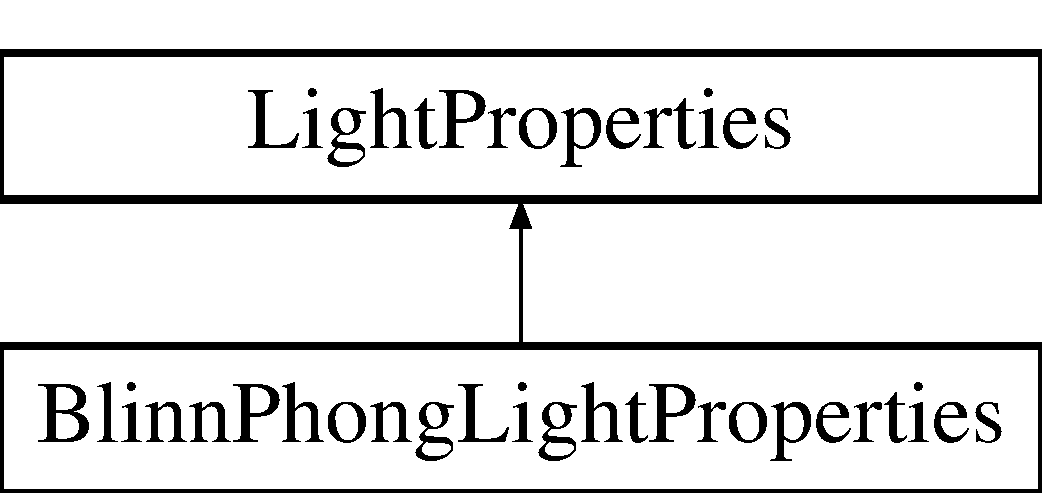
\includegraphics[height=2.000000cm]{struct_blinn_phong_light_properties}
\end{center}
\end{figure}
\subsection*{Public Attributes}
\begin{DoxyCompactItemize}
\item 
glm\+::vec4 \hyperlink{struct_blinn_phong_light_properties_aa12c81d848d370b8f79c9384d9fafec0}{diffuse\+Color}
\item 
glm\+::vec4 \hyperlink{struct_blinn_phong_light_properties_a815238c4f235333affb85f949ff8df06}{specular\+Color}
\end{DoxyCompactItemize}


\subsection{Detailed Description}


Definition at line 8 of file Blinn\+Phong\+Light\+Properties.\+h.



\subsection{Member Data Documentation}
\hypertarget{struct_blinn_phong_light_properties_aa12c81d848d370b8f79c9384d9fafec0}{}\index{Blinn\+Phong\+Light\+Properties@{Blinn\+Phong\+Light\+Properties}!diffuse\+Color@{diffuse\+Color}}
\index{diffuse\+Color@{diffuse\+Color}!Blinn\+Phong\+Light\+Properties@{Blinn\+Phong\+Light\+Properties}}
\subsubsection[{diffuse\+Color}]{\setlength{\rightskip}{0pt plus 5cm}glm\+::vec4 Blinn\+Phong\+Light\+Properties\+::diffuse\+Color}\label{struct_blinn_phong_light_properties_aa12c81d848d370b8f79c9384d9fafec0}


Definition at line 9 of file Blinn\+Phong\+Light\+Properties.\+h.

\hypertarget{struct_blinn_phong_light_properties_a815238c4f235333affb85f949ff8df06}{}\index{Blinn\+Phong\+Light\+Properties@{Blinn\+Phong\+Light\+Properties}!specular\+Color@{specular\+Color}}
\index{specular\+Color@{specular\+Color}!Blinn\+Phong\+Light\+Properties@{Blinn\+Phong\+Light\+Properties}}
\subsubsection[{specular\+Color}]{\setlength{\rightskip}{0pt plus 5cm}glm\+::vec4 Blinn\+Phong\+Light\+Properties\+::specular\+Color}\label{struct_blinn_phong_light_properties_a815238c4f235333affb85f949ff8df06}


Definition at line 10 of file Blinn\+Phong\+Light\+Properties.\+h.



The documentation for this struct was generated from the following file\+:\begin{DoxyCompactItemize}
\item 
/\+Users/michaelbao/\+Phys\+B\+A\+M/\+Courses/2015/cs148/cs148opengl4/source/common/\+Scene/\+Light/\+Properties/\+Blinn\+Phong/\hyperlink{_blinn_phong_light_properties_8h}{Blinn\+Phong\+Light\+Properties.\+h}\end{DoxyCompactItemize}

\hypertarget{class_blinn_phong_shader}{}\section{Blinn\+Phong\+Shader Class Reference}
\label{class_blinn_phong_shader}\index{Blinn\+Phong\+Shader@{Blinn\+Phong\+Shader}}
Inheritance diagram for Blinn\+Phong\+Shader\+:\begin{figure}[H]
\begin{center}
\leavevmode
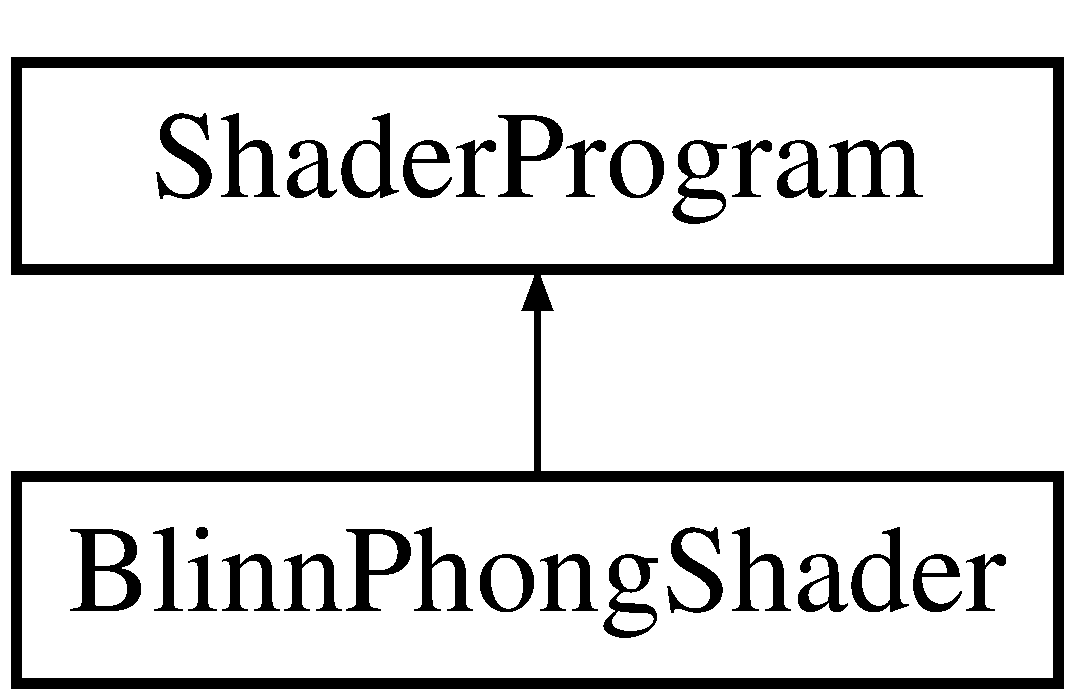
\includegraphics[height=2.000000cm]{class_blinn_phong_shader}
\end{center}
\end{figure}
\subsection*{Classes}
\begin{DoxyCompactItemize}
\item 
struct \hyperlink{struct_blinn_phong_shader_1_1_texture_slots}{Texture\+Slots}
\end{DoxyCompactItemize}
\subsection*{Public Member Functions}
\begin{DoxyCompactItemize}
\item 
\hypertarget{class_blinn_phong_shader_a2a13c983ffcc8d95ffe1a431bb2b1fb6}{}{\bfseries Blinn\+Phong\+Shader} (const std\+::unordered\+\_\+map$<$ G\+Lenum, std\+::string $>$ \&input\+Shaders, G\+Lenum lighting\+Stage)\label{class_blinn_phong_shader_a2a13c983ffcc8d95ffe1a431bb2b1fb6}

\item 
\hypertarget{class_blinn_phong_shader_a9e4a7358ce59f7fa77ed872eb15eabe7}{}virtual void {\bfseries Setup\+Shader\+Lighting} (const class \hyperlink{class_light}{Light} $\ast$light) const \label{class_blinn_phong_shader_a9e4a7358ce59f7fa77ed872eb15eabe7}

\item 
\hypertarget{class_blinn_phong_shader_ade1dfa6ceb0b2650b2ca3b849ee875ac}{}virtual void {\bfseries Setup\+Shader\+Materials} () const \label{class_blinn_phong_shader_ade1dfa6ceb0b2650b2ca3b849ee875ac}

\item 
\hypertarget{class_blinn_phong_shader_a0e3e2e1d5981f173a72e82d0ef4d643d}{}virtual void {\bfseries Setup\+Shader\+Camera} (const class \hyperlink{class_camera}{Camera} $\ast$camera) const \label{class_blinn_phong_shader_a0e3e2e1d5981f173a72e82d0ef4d643d}

\item 
\hypertarget{class_blinn_phong_shader_a610957f435f1ef817e7d2c4350e55181}{}virtual void {\bfseries Set\+Diffuse} (glm\+::vec4 in\+Diffuse)\label{class_blinn_phong_shader_a610957f435f1ef817e7d2c4350e55181}

\item 
\hypertarget{class_blinn_phong_shader_a6567423da36050cc1567919707e8be72}{}virtual void {\bfseries Set\+Specular} (glm\+::vec4 in\+Specular, float in\+Shininess)\label{class_blinn_phong_shader_a6567423da36050cc1567919707e8be72}

\item 
\hypertarget{class_blinn_phong_shader_a0f8c1c478525dd662922597ea7d9c4ac}{}virtual void {\bfseries Set\+Ambient} (glm\+::vec4 in\+Ambient)\label{class_blinn_phong_shader_a0f8c1c478525dd662922597ea7d9c4ac}

\item 
\hypertarget{class_blinn_phong_shader_aa9c8908b300ce1451887945fb961d3b2}{}virtual void {\bfseries Set\+Texture} (Texture\+Slots\+::\+Type slot, std\+::shared\+\_\+ptr$<$ class \hyperlink{class_texture}{Texture} $>$ input\+Texture)\label{class_blinn_phong_shader_aa9c8908b300ce1451887945fb961d3b2}

\end{DoxyCompactItemize}
\subsection*{Static Public Member Functions}
\begin{DoxyCompactItemize}
\item 
\hypertarget{class_blinn_phong_shader_a44f9413ef4896886b67b12c8809e5cd9}{}static std\+::unique\+\_\+ptr$<$ struct \hyperlink{struct_blinn_phong_light_properties}{Blinn\+Phong\+Light\+Properties} $>$ {\bfseries Create\+Light\+Properties} ()\label{class_blinn_phong_shader_a44f9413ef4896886b67b12c8809e5cd9}

\end{DoxyCompactItemize}
\subsection*{Protected Member Functions}
\begin{DoxyCompactItemize}
\item 
\hypertarget{class_blinn_phong_shader_ab620e8e40408c63f465af866e5ca9ef7}{}virtual void {\bfseries Update\+Material\+Block} () const \label{class_blinn_phong_shader_ab620e8e40408c63f465af866e5ca9ef7}

\item 
\hypertarget{class_blinn_phong_shader_aca3ae20f36d92b4e9b64ca4ae51a49f2}{}virtual void {\bfseries Update\+Attenuation\+Uniforms} (const class \hyperlink{class_light}{Light} $\ast$light) const \label{class_blinn_phong_shader_aca3ae20f36d92b4e9b64ca4ae51a49f2}

\end{DoxyCompactItemize}
\subsection*{Protected Attributes}
\begin{DoxyCompactItemize}
\item 
\hypertarget{class_blinn_phong_shader_ae74d0446ec1a871ca57caf002f52e20c}{}glm\+::vec4 {\bfseries diffuse}\label{class_blinn_phong_shader_ae74d0446ec1a871ca57caf002f52e20c}

\item 
\hypertarget{class_blinn_phong_shader_a7adce7364e850b9f232e058956f809b8}{}glm\+::vec4 {\bfseries specular}\label{class_blinn_phong_shader_a7adce7364e850b9f232e058956f809b8}

\item 
\hypertarget{class_blinn_phong_shader_ad499c2389d7007ecb4c03d5270314933}{}float {\bfseries shininess}\label{class_blinn_phong_shader_ad499c2389d7007ecb4c03d5270314933}

\item 
\hypertarget{class_blinn_phong_shader_af612b03df22b2bc9e37dcd85124ee9d2}{}glm\+::vec4 {\bfseries ambient}\label{class_blinn_phong_shader_af612b03df22b2bc9e37dcd85124ee9d2}

\item 
\hypertarget{class_blinn_phong_shader_a4dcd123c2284945734df697501dca5ea}{}G\+Luint {\bfseries material\+Block\+Location}\label{class_blinn_phong_shader_a4dcd123c2284945734df697501dca5ea}

\item 
\hypertarget{class_blinn_phong_shader_af38b3d042773f6568f0f6c227de85990}{}G\+Lint {\bfseries material\+Block\+Size}\label{class_blinn_phong_shader_af38b3d042773f6568f0f6c227de85990}

\item 
\hypertarget{class_blinn_phong_shader_a2b14622a5d0f8ca32c05cc387700692a}{}std\+::array$<$ G\+Luint, 4 $>$ {\bfseries material\+Indices}\label{class_blinn_phong_shader_a2b14622a5d0f8ca32c05cc387700692a}

\item 
\hypertarget{class_blinn_phong_shader_a145f22608d6e32a4ec5df39388ad0530}{}std\+::array$<$ G\+Lint, 4 $>$ {\bfseries material\+Offsets}\label{class_blinn_phong_shader_a145f22608d6e32a4ec5df39388ad0530}

\item 
\hypertarget{class_blinn_phong_shader_a85dbf4a8376a98570a06d9df17938cf4}{}G\+Luint {\bfseries material\+Buffer}\label{class_blinn_phong_shader_a85dbf4a8376a98570a06d9df17938cf4}

\item 
\hypertarget{class_blinn_phong_shader_a7c9644732d35c788d1c94f44b7783d83}{}std\+::vector$<$ G\+Lubyte $>$ {\bfseries material\+Storage}\label{class_blinn_phong_shader_a7c9644732d35c788d1c94f44b7783d83}

\end{DoxyCompactItemize}
\subsection*{Static Protected Attributes}
\begin{DoxyCompactItemize}
\item 
static const std\+::array$<$ const char $\ast$, 4 $>$ {\bfseries M\+A\+T\+E\+R\+I\+A\+L\+\_\+\+P\+R\+O\+P\+E\+R\+T\+Y\+\_\+\+N\+A\+M\+E\+S}
\item 
\hypertarget{class_blinn_phong_shader_a8c2a0ab9a26c0369ae3b45d5c9bd8f6b}{}static constexpr int {\bfseries M\+A\+T\+E\+R\+I\+A\+L\+\_\+\+B\+I\+N\+D\+I\+N\+G\+\_\+\+P\+O\+I\+N\+T} = 0\label{class_blinn_phong_shader_a8c2a0ab9a26c0369ae3b45d5c9bd8f6b}

\end{DoxyCompactItemize}
\subsection*{Additional Inherited Members}


\subsection{Detailed Description}


Definition at line 10 of file Blinn\+Phong\+Shader.\+h.



\subsection{Member Data Documentation}
\hypertarget{class_blinn_phong_shader_a3c74161a2680b16786f2c97f04e4ee20}{}\index{Blinn\+Phong\+Shader@{Blinn\+Phong\+Shader}!M\+A\+T\+E\+R\+I\+A\+L\+\_\+\+P\+R\+O\+P\+E\+R\+T\+Y\+\_\+\+N\+A\+M\+E\+S@{M\+A\+T\+E\+R\+I\+A\+L\+\_\+\+P\+R\+O\+P\+E\+R\+T\+Y\+\_\+\+N\+A\+M\+E\+S}}
\index{M\+A\+T\+E\+R\+I\+A\+L\+\_\+\+P\+R\+O\+P\+E\+R\+T\+Y\+\_\+\+N\+A\+M\+E\+S@{M\+A\+T\+E\+R\+I\+A\+L\+\_\+\+P\+R\+O\+P\+E\+R\+T\+Y\+\_\+\+N\+A\+M\+E\+S}!Blinn\+Phong\+Shader@{Blinn\+Phong\+Shader}}
\subsubsection[{M\+A\+T\+E\+R\+I\+A\+L\+\_\+\+P\+R\+O\+P\+E\+R\+T\+Y\+\_\+\+N\+A\+M\+E\+S}]{\setlength{\rightskip}{0pt plus 5cm}const std\+::array$<$ const char $\ast$, 4 $>$ Blinn\+Phong\+Shader\+::\+M\+A\+T\+E\+R\+I\+A\+L\+\_\+\+P\+R\+O\+P\+E\+R\+T\+Y\+\_\+\+N\+A\+M\+E\+S\hspace{0.3cm}{\ttfamily [static]}, {\ttfamily [protected]}}\label{class_blinn_phong_shader_a3c74161a2680b16786f2c97f04e4ee20}
{\bfseries Initial value\+:}
\begin{DoxyCode}
= \{
    \textcolor{stringliteral}{"InputMaterial.matDiffuse"}, 
    \textcolor{stringliteral}{"InputMaterial.matSpecular"}, 
    \textcolor{stringliteral}{"InputMaterial.matShininess"}, 
    \textcolor{stringliteral}{"InputMaterial.matAmbient"}
\}
\end{DoxyCode}


Definition at line 42 of file Blinn\+Phong\+Shader.\+h.



The documentation for this class was generated from the following files\+:\begin{DoxyCompactItemize}
\item 
/\+Users/michaelbao/workspace/cs148opengl4/source/common/\+Rendering/\+Shaders/Blinn\+Phong\+Shader.\+h\item 
/\+Users/michaelbao/workspace/cs148opengl4/source/common/\+Rendering/\+Shaders/Blinn\+Phong\+Shader.\+cpp\end{DoxyCompactItemize}

\hypertarget{class_camera}{}\section{Camera Class Reference}
\label{class_camera}\index{Camera@{Camera}}
Inheritance diagram for Camera\+:\begin{figure}[H]
\begin{center}
\leavevmode
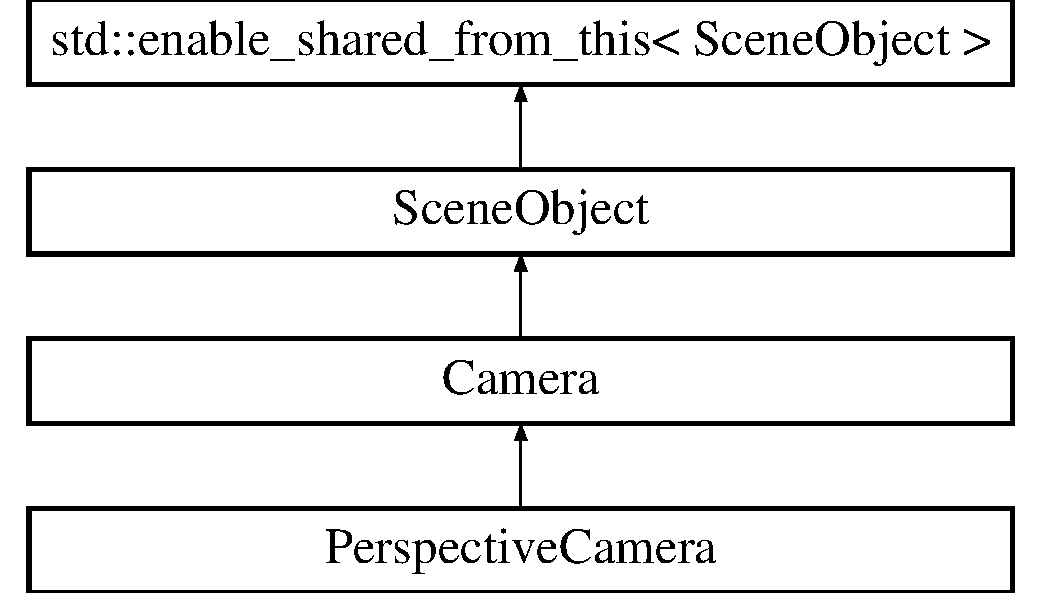
\includegraphics[height=4.000000cm]{class_camera}
\end{center}
\end{figure}
\subsection*{Public Member Functions}
\begin{DoxyCompactItemize}
\item 
\hypertarget{class_camera_a497efa3119ab4ae679d29badf6f25682}{}virtual glm\+::mat4 {\bfseries Get\+Projection\+Matrix} () const \label{class_camera_a497efa3119ab4ae679d29badf6f25682}

\end{DoxyCompactItemize}
\subsection*{Protected Member Functions}
\begin{DoxyCompactItemize}
\item 
\hypertarget{class_camera_aea640c892a3807671d8ca49616d96eda}{}virtual void {\bfseries Update\+Transformation\+Matrix} ()\label{class_camera_aea640c892a3807671d8ca49616d96eda}

\end{DoxyCompactItemize}
\subsection*{Additional Inherited Members}


\subsection{Detailed Description}


Definition at line 8 of file Camera.\+h.



The documentation for this class was generated from the following files\+:\begin{DoxyCompactItemize}
\item 
/\+Users/michaelbao/workspace/cs148opengl4/source/common/\+Scene/\+Camera/Camera.\+h\item 
/\+Users/michaelbao/workspace/cs148opengl4/source/common/\+Scene/\+Camera/Camera.\+cpp\end{DoxyCompactItemize}

\hypertarget{class_forward_renderer}{}\section{Forward\+Renderer Class Reference}
\label{class_forward_renderer}\index{Forward\+Renderer@{Forward\+Renderer}}


A multi-\/pass forward renderer with lights.  




{\ttfamily \#include $<$Forward\+Renderer.\+h$>$}

Inheritance diagram for Forward\+Renderer\+:\begin{figure}[H]
\begin{center}
\leavevmode
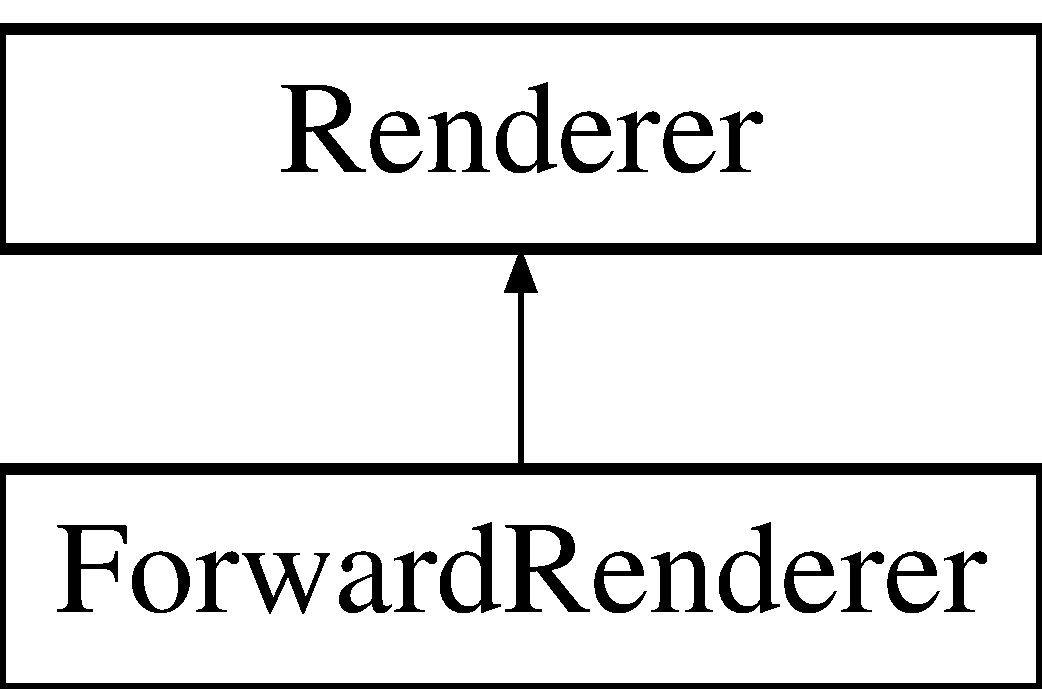
\includegraphics[height=2.000000cm]{class_forward_renderer}
\end{center}
\end{figure}
\subsection*{Public Member Functions}
\begin{DoxyCompactItemize}
\item 
\hyperlink{class_forward_renderer_af8ed84e45085c4dc60d565fcc3c198d1}{Forward\+Renderer} (std\+::shared\+\_\+ptr$<$ class \hyperlink{class_scene}{Scene} $>$ input\+Scene, std\+::shared\+\_\+ptr$<$ class \hyperlink{class_camera}{Camera} $>$ input\+Camera)
\begin{DoxyCompactList}\small\item\em Stores the input scene and the input camera for use for rendering. \end{DoxyCompactList}\item 
virtual \hyperlink{class_forward_renderer_ab27ea6139730631d79488cec3c564597}{$\sim$\+Forward\+Renderer} ()
\begin{DoxyCompactList}\small\item\em Just a day in the life of a destructor. \end{DoxyCompactList}\item 
virtual void \hyperlink{class_forward_renderer_a99c523e11a4335d061da8bdba51f1c9a}{Initialize} ()
\begin{DoxyCompactList}\small\item\em Loads the data that the forward renderer needs. \end{DoxyCompactList}\item 
virtual void \hyperlink{class_forward_renderer_a3693c5cd68afffc14652f24fcdc62abc}{Render} ()
\begin{DoxyCompactList}\small\item\em Renders a frame using a multi-\/pass forward renderer with all the lights in the scene. \end{DoxyCompactList}\end{DoxyCompactItemize}
\subsection*{Protected Attributes}
\begin{DoxyCompactItemize}
\item 
std\+::shared\+\_\+ptr$<$ class \hyperlink{class_shader_program}{Shader\+Program} $>$ \hyperlink{class_forward_renderer_a8f703bc4c646416804bc82f4d220a648}{depth\+Prepass\+Shader}
\begin{DoxyCompactList}\small\item\em The depth prepass shader. \end{DoxyCompactList}\end{DoxyCompactItemize}


\subsection{Detailed Description}
A multi-\/pass forward renderer with lights. 

More details about what a multi-\/pass forward renderer is can be found in the documentation for the \hyperlink{class_forward_renderer_a3693c5cd68afffc14652f24fcdc62abc}{Render()} function. Do note that this class will not support transparent objects out of the box! You will have to find a way to handle them if you want to display transparent objects properly. 

Definition at line 13 of file Forward\+Renderer.\+h.



\subsection{Constructor \& Destructor Documentation}
\hypertarget{class_forward_renderer_af8ed84e45085c4dc60d565fcc3c198d1}{}\index{Forward\+Renderer@{Forward\+Renderer}!Forward\+Renderer@{Forward\+Renderer}}
\index{Forward\+Renderer@{Forward\+Renderer}!Forward\+Renderer@{Forward\+Renderer}}
\subsubsection[{Forward\+Renderer}]{\setlength{\rightskip}{0pt plus 5cm}Forward\+Renderer\+::\+Forward\+Renderer (
\begin{DoxyParamCaption}
\item[{std\+::shared\+\_\+ptr$<$ class {\bf Scene} $>$}]{input\+Scene, }
\item[{std\+::shared\+\_\+ptr$<$ class {\bf Camera} $>$}]{input\+Camera}
\end{DoxyParamCaption}
)}\label{class_forward_renderer_af8ed84e45085c4dc60d565fcc3c198d1}


Stores the input scene and the input camera for use for rendering. 

Calls the base class constructor, \hyperlink{class_renderer_adc8ce31cd649bdf220ca8355809b1d06}{Renderer\+::\+Renderer()}. 

Definition at line 10 of file Forward\+Renderer.\+cpp.

\hypertarget{class_forward_renderer_ab27ea6139730631d79488cec3c564597}{}\index{Forward\+Renderer@{Forward\+Renderer}!````~Forward\+Renderer@{$\sim$\+Forward\+Renderer}}
\index{````~Forward\+Renderer@{$\sim$\+Forward\+Renderer}!Forward\+Renderer@{Forward\+Renderer}}
\subsubsection[{$\sim$\+Forward\+Renderer}]{\setlength{\rightskip}{0pt plus 5cm}Forward\+Renderer\+::$\sim$\+Forward\+Renderer (
\begin{DoxyParamCaption}
{}
\end{DoxyParamCaption}
)\hspace{0.3cm}{\ttfamily [virtual]}}\label{class_forward_renderer_ab27ea6139730631d79488cec3c564597}


Just a day in the life of a destructor. 



Definition at line 15 of file Forward\+Renderer.\+cpp.



\subsection{Member Function Documentation}
\hypertarget{class_forward_renderer_a99c523e11a4335d061da8bdba51f1c9a}{}\index{Forward\+Renderer@{Forward\+Renderer}!Initialize@{Initialize}}
\index{Initialize@{Initialize}!Forward\+Renderer@{Forward\+Renderer}}
\subsubsection[{Initialize}]{\setlength{\rightskip}{0pt plus 5cm}void Forward\+Renderer\+::\+Initialize (
\begin{DoxyParamCaption}
{}
\end{DoxyParamCaption}
)\hspace{0.3cm}{\ttfamily [virtual]}}\label{class_forward_renderer_a99c523e11a4335d061da8bdba51f1c9a}


Loads the data that the forward renderer needs. 

Loads the depth prepass shader. See the documentation of \hyperlink{class_forward_renderer_a3693c5cd68afffc14652f24fcdc62abc}{Render()} for why it is necessary. 

Implements \hyperlink{class_renderer_a7cb221f355f181d84d66e8c09f50f04a}{Renderer}.



Definition at line 19 of file Forward\+Renderer.\+cpp.

\hypertarget{class_forward_renderer_a3693c5cd68afffc14652f24fcdc62abc}{}\index{Forward\+Renderer@{Forward\+Renderer}!Render@{Render}}
\index{Render@{Render}!Forward\+Renderer@{Forward\+Renderer}}
\subsubsection[{Render}]{\setlength{\rightskip}{0pt plus 5cm}void Forward\+Renderer\+::\+Render (
\begin{DoxyParamCaption}
{}
\end{DoxyParamCaption}
)\hspace{0.3cm}{\ttfamily [virtual]}}\label{class_forward_renderer_a3693c5cd68afffc14652f24fcdc62abc}


Renders a frame using a multi-\/pass forward renderer with all the lights in the scene. 

Note that in the multi-\/pass forward renderer, there is no limit to how many lights you may use; however, once the number of lights becomes too high, you will start to see a significant drop in frames per second. In our implementation of the multi-\/pass forward renderer, assuming that there are $N$ lights, the renderer will perform $ N + 2 $ passes through every object in the scene. For every draw call, the multi-\/pass forward renderer will perform additive blending of both the R\+G\+B and alpha channels to compute the new color in the color buffer. The render pass stages are as follows\+:


\begin{DoxyEnumerate}
\item The depth preprocess stage. Without this stage, some objects will transparent even if they are not actually. Let\textquotesingle{}s say a relative large and complex object has parts that are facing towards the camera but are occluded. Then let\textquotesingle{}s say that the light vertex/fragment shader processes that part first and then processes the occluder parts later. With additive blending turned on, the colors will be mixed! Turning additive blending is not an option for a multi-\/pass forward renderer. Instead what we want to do is to perform an initial \char`\"{}depth preprocess\char`\"{} pass through every object in the scene. By doing this, we write the final depth of an object to the depth buffer. In the subsequent render passes, we will only write to the color buffer is the depth value is less than or equal to the value already stored in the depth buffer. Since we ran the depth preprocess pass on E\+V\+E\+R\+Y object in the scene, we are guaranteed that the value stored in the depth buffer is the smallest possible value for that pixel. So if a render pass passes the depth buffer check, it can know for sure that it is safe to write to the color buffer and that there won\textquotesingle{}t be another object occluding it. It is important to note that depth is stored as a floating point value and with floating point values comes numerical imprecision which can result in \href{https://en.wikipedia.org/wiki/Z-fighting}{\tt z-\/fighting}. As a result, we use \href{https://www.opengl.org/sdk/docs/man/html/glPolygonOffset.xhtml}{\tt gl\+Polygon\+Offset} to offset the depth values ever so slightly to prevent z-\/fighting from occurring. The amount that we offset $\sim$should$\sim$ not be enough to cause problems with fragments passing the depth buffer test that otherwise should not.
\item The \char`\"{}global lighting\char`\"{} phase. This phase takes care of the ambient color of the material (Note\+: it might make more sense for the ambient color be a property of the light and not the material). Regardless, this phase will take care of the color that should only be added to the object once regardless of how many lights shine upon it. Good examples of things that would go in this stage are the ambient and emissive colors.
\item Finally, the rest of the lighting passes are dedicated to performing a normal render pass with a light in the scene. The rendering object in question is queried for the correct shader to use, the shader is then setup by the rendering object and the scene object, and finally the object is rendered and the resulting fragment colors are correctly blended into the color buffer.
\end{DoxyEnumerate}

Still confused? Ask on Piazza! 

Implements \hyperlink{class_renderer_a38623da22aa718cfa41e2514ebd269f5}{Renderer}.



Definition at line 28 of file Forward\+Renderer.\+cpp.



\subsection{Member Data Documentation}
\hypertarget{class_forward_renderer_a8f703bc4c646416804bc82f4d220a648}{}\index{Forward\+Renderer@{Forward\+Renderer}!depth\+Prepass\+Shader@{depth\+Prepass\+Shader}}
\index{depth\+Prepass\+Shader@{depth\+Prepass\+Shader}!Forward\+Renderer@{Forward\+Renderer}}
\subsubsection[{depth\+Prepass\+Shader}]{\setlength{\rightskip}{0pt plus 5cm}std\+::shared\+\_\+ptr$<$class {\bf Shader\+Program}$>$ Forward\+Renderer\+::depth\+Prepass\+Shader\hspace{0.3cm}{\ttfamily [protected]}}\label{class_forward_renderer_a8f703bc4c646416804bc82f4d220a648}


The depth prepass shader. 

The depth prepass shader is constructed from the shaders loaded in \char`\"{}shaders/required/pass\char`\"{}. The vertex shader applies the M\+V\+P transformations to the input vertex and stores it in gl\+\_\+\+Position. The fragment shader will write (0, 0, 0, 0) to the color buffer to not affect the results of the following render passes. 

Definition at line 70 of file Forward\+Renderer.\+h.



The documentation for this class was generated from the following files\+:\begin{DoxyCompactItemize}
\item 
/\+Users/michaelbao/workspace/cs148opengl4/source/common/\+Rendering/\hyperlink{_forward_renderer_8h}{Forward\+Renderer.\+h}\item 
/\+Users/michaelbao/workspace/cs148opengl4/source/common/\+Rendering/\hyperlink{_forward_renderer_8cpp}{Forward\+Renderer.\+cpp}\end{DoxyCompactItemize}

\hypertarget{class_light}{}\section{Light Class Reference}
\label{class_light}\index{Light@{Light}}


{\ttfamily \#include $<$Light.\+h$>$}

Inheritance diagram for Light\+:\begin{figure}[H]
\begin{center}
\leavevmode
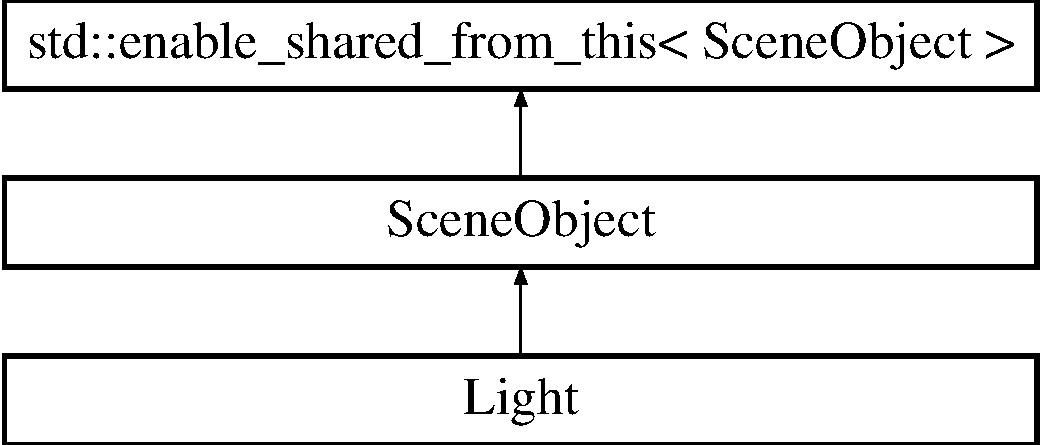
\includegraphics[height=3.000000cm]{class_light}
\end{center}
\end{figure}
\subsection*{Public Types}
\begin{DoxyCompactItemize}
\item 
enum \hyperlink{class_light_a661d9480e01af8b1612860b9630ef5f8}{Light\+Type} \{ \hyperlink{class_light_a661d9480e01af8b1612860b9630ef5f8a6eecfba72d12922ee1dead07a0ef3334}{Light\+Type\+::\+G\+L\+O\+B\+A\+L} = 0, 
\hyperlink{class_light_a661d9480e01af8b1612860b9630ef5f8aaebdbcb765394d25d6a604589a890f82}{Light\+Type\+::\+P\+O\+I\+N\+T}
 \}
\end{DoxyCompactItemize}
\subsection*{Public Member Functions}
\begin{DoxyCompactItemize}
\item 
\hyperlink{class_light_adca12f0d5470bc3f2e6e77233ab3dcf1}{Light} (std\+::unique\+\_\+ptr$<$ struct \hyperlink{struct_light_properties}{Light\+Properties} $>$ in\+Properties, \hyperlink{class_light_a661d9480e01af8b1612860b9630ef5f8}{Light\+Type} type=\hyperlink{class_light_a661d9480e01af8b1612860b9630ef5f8aaebdbcb765394d25d6a604589a890f82}{Light\+Type\+::\+P\+O\+I\+N\+T})
\item 
virtual \hyperlink{class_light_ad0e59fad13bb6cfadc25b2c477e9ddc7}{$\sim$\+Light} ()
\item 
void \hyperlink{class_light_a2d3f34b821c0cb0b5baa664ee91d309f}{Get\+Attenuation} (float \&constant, float \&linear, float \&quadratic) const 
\item 
\hyperlink{class_light_a661d9480e01af8b1612860b9630ef5f8}{Light\+Type} \hyperlink{class_light_a393ede80ccba5f4314135011a665afab}{Get\+Light\+Type} () const 
\item 
const struct \hyperlink{struct_light_properties}{Light\+Properties} $\ast$ \hyperlink{class_light_a074230bc62c5bf705bc39c1de64474c0}{Get\+Properties\+Raw} () const 
\item 
virtual void \hyperlink{class_light_a360ea479af434502737f6b5c0b0ff3d9}{Setup\+Shader\+Uniforms} (const class \hyperlink{class_shader_program}{Shader\+Program} $\ast$program) const 
\end{DoxyCompactItemize}
\subsection*{Private Attributes}
\begin{DoxyCompactItemize}
\item 
std\+::unique\+\_\+ptr$<$ struct \hyperlink{struct_light_properties}{Light\+Properties} $>$ \hyperlink{class_light_a74eba4cac1cc27e741230fbda32fceef}{properties}
\item 
\hyperlink{class_light_a661d9480e01af8b1612860b9630ef5f8}{Light\+Type} \hyperlink{class_light_ab0c279c927973443f7b52fc924b489aa}{light\+Type}
\item 
float \hyperlink{class_light_afef6c00a21aa16dc6cc7a7fb1639d2fa}{constant\+Attenuation}
\item 
float \hyperlink{class_light_afcb2da592197efae015ae16c1c5bfceb}{linear\+Attenuation}
\item 
float \hyperlink{class_light_a0f24dde11cbbd12d0f0309e189f3640c}{quadratic\+Attenuation}
\end{DoxyCompactItemize}
\subsection*{Static Private Attributes}
\begin{DoxyCompactItemize}
\item 
static const std\+::string \hyperlink{class_light_ab2d40f6c364cf728d03a90ff885e37cb}{L\+I\+G\+H\+T\+\_\+\+U\+N\+I\+F\+O\+R\+M\+\_\+\+N\+A\+M\+E} = \char`\"{}point\+Light\char`\"{}
\end{DoxyCompactItemize}
\subsection*{Additional Inherited Members}


\subsection{Detailed Description}


Definition at line 9 of file Light.\+h.



\subsection{Member Enumeration Documentation}
\hypertarget{class_light_a661d9480e01af8b1612860b9630ef5f8}{}\index{Light@{Light}!Light\+Type@{Light\+Type}}
\index{Light\+Type@{Light\+Type}!Light@{Light}}
\subsubsection[{Light\+Type}]{\setlength{\rightskip}{0pt plus 5cm}enum {\bf Light\+::\+Light\+Type}\hspace{0.3cm}{\ttfamily [strong]}}\label{class_light_a661d9480e01af8b1612860b9630ef5f8}
\begin{Desc}
\item[Enumerator]\par
\begin{description}
\index{G\+L\+O\+B\+A\+L@{G\+L\+O\+B\+A\+L}!Light@{Light}}\index{Light@{Light}!G\+L\+O\+B\+A\+L@{G\+L\+O\+B\+A\+L}}\item[{\em 
\hypertarget{class_light_a661d9480e01af8b1612860b9630ef5f8a6eecfba72d12922ee1dead07a0ef3334}{}G\+L\+O\+B\+A\+L\label{class_light_a661d9480e01af8b1612860b9630ef5f8a6eecfba72d12922ee1dead07a0ef3334}
}]\index{P\+O\+I\+N\+T@{P\+O\+I\+N\+T}!Light@{Light}}\index{Light@{Light}!P\+O\+I\+N\+T@{P\+O\+I\+N\+T}}\item[{\em 
\hypertarget{class_light_a661d9480e01af8b1612860b9630ef5f8aaebdbcb765394d25d6a604589a890f82}{}P\+O\+I\+N\+T\label{class_light_a661d9480e01af8b1612860b9630ef5f8aaebdbcb765394d25d6a604589a890f82}
}]\end{description}
\end{Desc}


Definition at line 12 of file Light.\+h.



\subsection{Constructor \& Destructor Documentation}
\hypertarget{class_light_adca12f0d5470bc3f2e6e77233ab3dcf1}{}\index{Light@{Light}!Light@{Light}}
\index{Light@{Light}!Light@{Light}}
\subsubsection[{Light}]{\setlength{\rightskip}{0pt plus 5cm}Light\+::\+Light (
\begin{DoxyParamCaption}
\item[{std\+::unique\+\_\+ptr$<$ struct {\bf Light\+Properties} $>$}]{in\+Properties, }
\item[{{\bf Light\+Type}}]{type = {\ttfamily {\bf Light\+Type\+::\+P\+O\+I\+N\+T}}}
\end{DoxyParamCaption}
)}\label{class_light_adca12f0d5470bc3f2e6e77233ab3dcf1}


Definition at line 7 of file Light.\+cpp.

\hypertarget{class_light_ad0e59fad13bb6cfadc25b2c477e9ddc7}{}\index{Light@{Light}!````~Light@{$\sim$\+Light}}
\index{````~Light@{$\sim$\+Light}!Light@{Light}}
\subsubsection[{$\sim$\+Light}]{\setlength{\rightskip}{0pt plus 5cm}Light\+::$\sim$\+Light (
\begin{DoxyParamCaption}
{}
\end{DoxyParamCaption}
)\hspace{0.3cm}{\ttfamily [virtual]}}\label{class_light_ad0e59fad13bb6cfadc25b2c477e9ddc7}


Definition at line 12 of file Light.\+cpp.



\subsection{Member Function Documentation}
\hypertarget{class_light_a2d3f34b821c0cb0b5baa664ee91d309f}{}\index{Light@{Light}!Get\+Attenuation@{Get\+Attenuation}}
\index{Get\+Attenuation@{Get\+Attenuation}!Light@{Light}}
\subsubsection[{Get\+Attenuation}]{\setlength{\rightskip}{0pt plus 5cm}void Light\+::\+Get\+Attenuation (
\begin{DoxyParamCaption}
\item[{float \&}]{constant, }
\item[{float \&}]{linear, }
\item[{float \&}]{quadratic}
\end{DoxyParamCaption}
) const}\label{class_light_a2d3f34b821c0cb0b5baa664ee91d309f}


Definition at line 16 of file Light.\+cpp.

\hypertarget{class_light_a393ede80ccba5f4314135011a665afab}{}\index{Light@{Light}!Get\+Light\+Type@{Get\+Light\+Type}}
\index{Get\+Light\+Type@{Get\+Light\+Type}!Light@{Light}}
\subsubsection[{Get\+Light\+Type}]{\setlength{\rightskip}{0pt plus 5cm}{\bf Light\+Type} Light\+::\+Get\+Light\+Type (
\begin{DoxyParamCaption}
{}
\end{DoxyParamCaption}
) const\hspace{0.3cm}{\ttfamily [inline]}}\label{class_light_a393ede80ccba5f4314135011a665afab}


Definition at line 22 of file Light.\+h.

\hypertarget{class_light_a074230bc62c5bf705bc39c1de64474c0}{}\index{Light@{Light}!Get\+Properties\+Raw@{Get\+Properties\+Raw}}
\index{Get\+Properties\+Raw@{Get\+Properties\+Raw}!Light@{Light}}
\subsubsection[{Get\+Properties\+Raw}]{\setlength{\rightskip}{0pt plus 5cm}const {\bf Light\+Properties} $\ast$ Light\+::\+Get\+Properties\+Raw (
\begin{DoxyParamCaption}
{}
\end{DoxyParamCaption}
) const}\label{class_light_a074230bc62c5bf705bc39c1de64474c0}


Definition at line 23 of file Light.\+cpp.

\hypertarget{class_light_a360ea479af434502737f6b5c0b0ff3d9}{}\index{Light@{Light}!Setup\+Shader\+Uniforms@{Setup\+Shader\+Uniforms}}
\index{Setup\+Shader\+Uniforms@{Setup\+Shader\+Uniforms}!Light@{Light}}
\subsubsection[{Setup\+Shader\+Uniforms}]{\setlength{\rightskip}{0pt plus 5cm}void Light\+::\+Setup\+Shader\+Uniforms (
\begin{DoxyParamCaption}
\item[{const class {\bf Shader\+Program} $\ast$}]{program}
\end{DoxyParamCaption}
) const\hspace{0.3cm}{\ttfamily [virtual]}}\label{class_light_a360ea479af434502737f6b5c0b0ff3d9}


Definition at line 28 of file Light.\+cpp.



\subsection{Member Data Documentation}
\hypertarget{class_light_afef6c00a21aa16dc6cc7a7fb1639d2fa}{}\index{Light@{Light}!constant\+Attenuation@{constant\+Attenuation}}
\index{constant\+Attenuation@{constant\+Attenuation}!Light@{Light}}
\subsubsection[{constant\+Attenuation}]{\setlength{\rightskip}{0pt plus 5cm}float Light\+::constant\+Attenuation\hspace{0.3cm}{\ttfamily [private]}}\label{class_light_afef6c00a21aa16dc6cc7a7fb1639d2fa}


Definition at line 34 of file Light.\+h.

\hypertarget{class_light_ab2d40f6c364cf728d03a90ff885e37cb}{}\index{Light@{Light}!L\+I\+G\+H\+T\+\_\+\+U\+N\+I\+F\+O\+R\+M\+\_\+\+N\+A\+M\+E@{L\+I\+G\+H\+T\+\_\+\+U\+N\+I\+F\+O\+R\+M\+\_\+\+N\+A\+M\+E}}
\index{L\+I\+G\+H\+T\+\_\+\+U\+N\+I\+F\+O\+R\+M\+\_\+\+N\+A\+M\+E@{L\+I\+G\+H\+T\+\_\+\+U\+N\+I\+F\+O\+R\+M\+\_\+\+N\+A\+M\+E}!Light@{Light}}
\subsubsection[{L\+I\+G\+H\+T\+\_\+\+U\+N\+I\+F\+O\+R\+M\+\_\+\+N\+A\+M\+E}]{\setlength{\rightskip}{0pt plus 5cm}const std\+::string Light\+::\+L\+I\+G\+H\+T\+\_\+\+U\+N\+I\+F\+O\+R\+M\+\_\+\+N\+A\+M\+E = \char`\"{}point\+Light\char`\"{}\hspace{0.3cm}{\ttfamily [static]}, {\ttfamily [private]}}\label{class_light_ab2d40f6c364cf728d03a90ff885e37cb}


Definition at line 28 of file Light.\+h.

\hypertarget{class_light_ab0c279c927973443f7b52fc924b489aa}{}\index{Light@{Light}!light\+Type@{light\+Type}}
\index{light\+Type@{light\+Type}!Light@{Light}}
\subsubsection[{light\+Type}]{\setlength{\rightskip}{0pt plus 5cm}{\bf Light\+Type} Light\+::light\+Type\hspace{0.3cm}{\ttfamily [private]}}\label{class_light_ab0c279c927973443f7b52fc924b489aa}


Definition at line 31 of file Light.\+h.

\hypertarget{class_light_afcb2da592197efae015ae16c1c5bfceb}{}\index{Light@{Light}!linear\+Attenuation@{linear\+Attenuation}}
\index{linear\+Attenuation@{linear\+Attenuation}!Light@{Light}}
\subsubsection[{linear\+Attenuation}]{\setlength{\rightskip}{0pt plus 5cm}float Light\+::linear\+Attenuation\hspace{0.3cm}{\ttfamily [private]}}\label{class_light_afcb2da592197efae015ae16c1c5bfceb}


Definition at line 35 of file Light.\+h.

\hypertarget{class_light_a74eba4cac1cc27e741230fbda32fceef}{}\index{Light@{Light}!properties@{properties}}
\index{properties@{properties}!Light@{Light}}
\subsubsection[{properties}]{\setlength{\rightskip}{0pt plus 5cm}std\+::unique\+\_\+ptr$<$struct {\bf Light\+Properties}$>$ Light\+::properties\hspace{0.3cm}{\ttfamily [private]}}\label{class_light_a74eba4cac1cc27e741230fbda32fceef}


Definition at line 29 of file Light.\+h.

\hypertarget{class_light_a0f24dde11cbbd12d0f0309e189f3640c}{}\index{Light@{Light}!quadratic\+Attenuation@{quadratic\+Attenuation}}
\index{quadratic\+Attenuation@{quadratic\+Attenuation}!Light@{Light}}
\subsubsection[{quadratic\+Attenuation}]{\setlength{\rightskip}{0pt plus 5cm}float Light\+::quadratic\+Attenuation\hspace{0.3cm}{\ttfamily [private]}}\label{class_light_a0f24dde11cbbd12d0f0309e189f3640c}


Definition at line 36 of file Light.\+h.



The documentation for this class was generated from the following files\+:\begin{DoxyCompactItemize}
\item 
/\+Users/michaelbao/workspace/cs148opengl4/source/common/\+Scene/\+Light/\hyperlink{_light_8h}{Light.\+h}\item 
/\+Users/michaelbao/workspace/cs148opengl4/source/common/\+Scene/\+Light/\hyperlink{_light_8cpp}{Light.\+cpp}\end{DoxyCompactItemize}

\hypertarget{struct_light_properties}{}\section{Light\+Properties Struct Reference}
\label{struct_light_properties}\index{Light\+Properties@{Light\+Properties}}
Inheritance diagram for Light\+Properties\+:\begin{figure}[H]
\begin{center}
\leavevmode
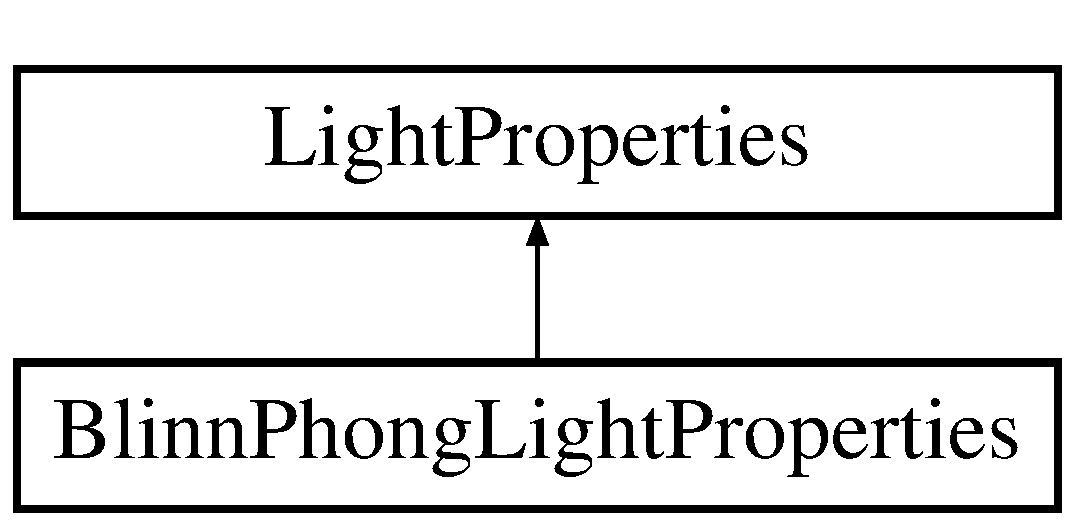
\includegraphics[height=2.000000cm]{struct_light_properties}
\end{center}
\end{figure}


\subsection{Detailed Description}


Definition at line 8 of file Light\+Properties.\+h.



The documentation for this struct was generated from the following file\+:\begin{DoxyCompactItemize}
\item 
/\+Users/michaelbao/workspace/cs148opengl4/source/common/\+Scene/\+Light/Light\+Properties.\+h\end{DoxyCompactItemize}

\hypertarget{class_media_layer}{}\section{Media\+Layer Class Reference}
\label{class_media_layer}\index{Media\+Layer@{Media\+Layer}}


Class that initializes the application and makes it ready to process Open\+G\+L commands.  




{\ttfamily \#include $<$Media\+Layer.\+h$>$}

\subsection*{Public Member Functions}
\begin{DoxyCompactItemize}
\item 
\hyperlink{class_media_layer_aea3b3bc36411af90517692b110d2829a}{Media\+Layer} (std\+::unique\+\_\+ptr$<$ \hyperlink{class_application}{Application} $>$ input\+App, std\+::unique\+\_\+ptr$<$ \hyperlink{class_renderer}{Renderer} $>$ input\+Renderer)
\begin{DoxyCompactList}\small\item\em Constructs a \hyperlink{class_media_layer}{Media\+Layer} object and readies the \hyperlink{class_application}{Application} and \hyperlink{class_renderer}{Renderer} for immediate use. \end{DoxyCompactList}\item 
\hyperlink{class_media_layer_a0c64e2d0a1c7b34b5457a0c57b69bbb1}{$\sim$\+Media\+Layer} ()
\begin{DoxyCompactList}\small\item\em A destructor. Carry on. \end{DoxyCompactList}\item 
bool \hyperlink{class_media_layer_a9f3b22b608b45efa23ebaebe17ae3a85}{Can\+Tick} () const 
\begin{DoxyCompactList}\small\item\em Whether or not the program should keep running. \end{DoxyCompactList}\item 
void \hyperlink{class_media_layer_a570ff8c3fc3e8f3e720d9dcebafba143}{Tick} (double delta\+Time, double current\+Time)
\begin{DoxyCompactList}\small\item\em Handles what happens every frame. \end{DoxyCompactList}\end{DoxyCompactItemize}
\subsection*{Private Member Functions}
\begin{DoxyCompactItemize}
\item 
void \hyperlink{class_media_layer_ad72130dbe963e351d5749a7f48b4ef97}{Initialize\+S\+D\+L} ()
\begin{DoxyCompactList}\small\item\em Initializes S\+D\+L. \end{DoxyCompactList}\item 
void \hyperlink{class_media_layer_abb3502cb44e707538741f55f5fe81361}{Initialize\+Open\+G\+L} ()
\begin{DoxyCompactList}\small\item\em Initializes Open\+G\+L. \end{DoxyCompactList}\end{DoxyCompactItemize}
\subsection*{Private Attributes}
\begin{DoxyCompactItemize}
\item 
std\+::unique\+\_\+ptr$<$ \hyperlink{class_application}{Application} $>$ \hyperlink{class_media_layer_a3cddf8a24527db756c3fe0534fce4f0c}{app}
\begin{DoxyCompactList}\small\item\em Underlying \hyperlink{class_application}{Application} to run. \end{DoxyCompactList}\item 
std\+::unique\+\_\+ptr$<$ \hyperlink{class_renderer}{Renderer} $>$ \hyperlink{class_media_layer_aee28804a7f4e1fb771b11e93b218e387}{renderer}
\begin{DoxyCompactList}\small\item\em Underlying \hyperlink{class_renderer}{Renderer} to run. \end{DoxyCompactList}\item 
S\+D\+L\+\_\+\+Window $\ast$ \hyperlink{class_media_layer_a769679df4457ecbe60e9668199e8788b}{sdl\+Window}
\begin{DoxyCompactList}\small\item\em Store a pointer to the sdl\+Window so we can clean this up later. \end{DoxyCompactList}\item 
bool \hyperlink{class_media_layer_ab577253a72d7d158badb3932f09e7d3f}{sdl\+Initialized}
\begin{DoxyCompactList}\small\item\em Set to true if \hyperlink{class_media_layer_ad72130dbe963e351d5749a7f48b4ef97}{Initialize\+S\+D\+L()} runs successfully. \end{DoxyCompactList}\item 
S\+D\+L\+\_\+\+G\+L\+Context \hyperlink{class_media_layer_a0e027d967e7c796efaed751e0b0a7090}{gl\+Context}
\begin{DoxyCompactList}\small\item\em Store the Open\+G\+L context so that we can clean it up later. \end{DoxyCompactList}\item 
bool \hyperlink{class_media_layer_abb67004f8dd82afd036233dfb225df3d}{opengl\+Initialized}
\begin{DoxyCompactList}\small\item\em Set to true after G\+L\+E\+W initialization succeeds. \end{DoxyCompactList}\end{DoxyCompactItemize}


\subsection{Detailed Description}
Class that initializes the application and makes it ready to process Open\+G\+L commands. 

This class \char`\"{}owns\char`\"{} the \hyperlink{class_application}{Application}. It will handle telling when the application and the renderer should do their per-\/frame actions as well as handling I/\+O events and passing it to the application. Should you ever decide to handle audio and networking this is the class that should own the respective handlers. 

Definition at line 21 of file Media\+Layer.\+h.



\subsection{Constructor \& Destructor Documentation}
\hypertarget{class_media_layer_aea3b3bc36411af90517692b110d2829a}{}\index{Media\+Layer@{Media\+Layer}!Media\+Layer@{Media\+Layer}}
\index{Media\+Layer@{Media\+Layer}!Media\+Layer@{Media\+Layer}}
\subsubsection[{Media\+Layer}]{\setlength{\rightskip}{0pt plus 5cm}Media\+Layer\+::\+Media\+Layer (
\begin{DoxyParamCaption}
\item[{std\+::unique\+\_\+ptr$<$ {\bf Application} $>$}]{input\+App, }
\item[{std\+::unique\+\_\+ptr$<$ {\bf Renderer} $>$}]{input\+Renderer}
\end{DoxyParamCaption}
)}\label{class_media_layer_aea3b3bc36411af90517692b110d2829a}


Constructs a \hyperlink{class_media_layer}{Media\+Layer} object and readies the \hyperlink{class_application}{Application} and \hyperlink{class_renderer}{Renderer} for immediate use. 

\begin{DoxyWarning}{Warning}
After passing in the std\+::unique\+\_\+ptr\textquotesingle{}s to \hyperlink{class_media_layer}{Media\+Layer}, you will no longer be able to use the previous std\+::unique\+\_\+ptr\textquotesingle{}s. For example, let\textquotesingle{}s say you have the unique pointers x and y and you call \hyperlink{class_media_layer}{Media\+Layer}(std\+::move(x), std\+::move(y)). After this call, x and y will N\+O L\+O\+N\+G\+E\+R B\+E V\+A\+L\+I\+D P\+O\+I\+N\+T\+E\+R\+S. D\+O N\+O\+T U\+S\+E T\+H\+E\+M. For more information about this, you will want to read more about \href{http://thbecker.net/articles/rvalue_references/section_01.html}{\tt R-\/\+Values} and \href{http://thbecker.net/articles/rvalue_references/section_02.html}{\tt move semantics}. 
\end{DoxyWarning}

\begin{DoxyParams}{Parameters}
{\em input\+App} & The unique pointer to the application. We will own this pointer. \\
\hline
{\em input\+Renderer} & The unique pointer to the renderer. We will own this pointer.\\
\hline
\end{DoxyParams}
This class assumes that the \hyperlink{class_application}{Application} and \hyperlink{class_renderer}{Renderer} are ready for use once the \hyperlink{class_media_layer}{Media\+Layer} is created. After passing them to the \hyperlink{class_media_layer}{Media\+Layer} constructor, you will no longer be able to modify them without doing some black magic within the \hyperlink{class_media_layer}{Media\+Layer}. 

Definition at line 4 of file Media\+Layer.\+cpp.

\hypertarget{class_media_layer_a0c64e2d0a1c7b34b5457a0c57b69bbb1}{}\index{Media\+Layer@{Media\+Layer}!````~Media\+Layer@{$\sim$\+Media\+Layer}}
\index{````~Media\+Layer@{$\sim$\+Media\+Layer}!Media\+Layer@{Media\+Layer}}
\subsubsection[{$\sim$\+Media\+Layer}]{\setlength{\rightskip}{0pt plus 5cm}Media\+Layer\+::$\sim$\+Media\+Layer (
\begin{DoxyParamCaption}
{}
\end{DoxyParamCaption}
)}\label{class_media_layer_a0c64e2d0a1c7b34b5457a0c57b69bbb1}


A destructor. Carry on. 



Definition at line 17 of file Media\+Layer.\+cpp.



\subsection{Member Function Documentation}
\hypertarget{class_media_layer_a9f3b22b608b45efa23ebaebe17ae3a85}{}\index{Media\+Layer@{Media\+Layer}!Can\+Tick@{Can\+Tick}}
\index{Can\+Tick@{Can\+Tick}!Media\+Layer@{Media\+Layer}}
\subsubsection[{Can\+Tick}]{\setlength{\rightskip}{0pt plus 5cm}bool Media\+Layer\+::\+Can\+Tick (
\begin{DoxyParamCaption}
{}
\end{DoxyParamCaption}
) const}\label{class_media_layer_a9f3b22b608b45efa23ebaebe17ae3a85}


Whether or not the program should keep running. 

The main loop will query \hyperlink{class_media_layer_a9f3b22b608b45efa23ebaebe17ae3a85}{Can\+Tick()} to see if the program should keep running. If S\+D\+L or Open\+G\+L fails, the program will immediately exit. Also, if the application wants to exit (i.\+e. \hyperlink{class_application_ae0019f2c58008791971e67f23f2d4182}{Application\+::\+Is\+Finished()}) is true, then the main loop will stop as well. 

Definition at line 101 of file Media\+Layer.\+cpp.

\hypertarget{class_media_layer_abb3502cb44e707538741f55f5fe81361}{}\index{Media\+Layer@{Media\+Layer}!Initialize\+Open\+G\+L@{Initialize\+Open\+G\+L}}
\index{Initialize\+Open\+G\+L@{Initialize\+Open\+G\+L}!Media\+Layer@{Media\+Layer}}
\subsubsection[{Initialize\+Open\+G\+L}]{\setlength{\rightskip}{0pt plus 5cm}void Media\+Layer\+::\+Initialize\+Open\+G\+L (
\begin{DoxyParamCaption}
{}
\end{DoxyParamCaption}
)\hspace{0.3cm}{\ttfamily [private]}}\label{class_media_layer_abb3502cb44e707538741f55f5fe81361}


Initializes Open\+G\+L. 

This function will not run if S\+D\+L was not initialized. If S\+D\+L was initialized, this function will request an Open\+G\+L context and then setup the Open\+G\+L function pointers using G\+L\+E\+W. If G\+L\+E\+W initialization succeeds, we will enable some sane defaults for rendering. 

Definition at line 44 of file Media\+Layer.\+cpp.

\hypertarget{class_media_layer_ad72130dbe963e351d5749a7f48b4ef97}{}\index{Media\+Layer@{Media\+Layer}!Initialize\+S\+D\+L@{Initialize\+S\+D\+L}}
\index{Initialize\+S\+D\+L@{Initialize\+S\+D\+L}!Media\+Layer@{Media\+Layer}}
\subsubsection[{Initialize\+S\+D\+L}]{\setlength{\rightskip}{0pt plus 5cm}void Media\+Layer\+::\+Initialize\+S\+D\+L (
\begin{DoxyParamCaption}
{}
\end{DoxyParamCaption}
)\hspace{0.3cm}{\ttfamily [private]}}\label{class_media_layer_ad72130dbe963e351d5749a7f48b4ef97}


Initializes S\+D\+L. 

This function will initialize S\+D\+L with \href{https://wiki.libsdl.org/SDL_Init}{\tt S\+D\+L\+\_\+\+Init} and create a window. The size of the window will initially be the value returned by \hyperlink{class_application_a3e9992f0ceae0d8beda7debccdb00534}{Application\+::\+Get\+Window\+Size()}. 

Definition at line 23 of file Media\+Layer.\+cpp.

\hypertarget{class_media_layer_a570ff8c3fc3e8f3e720d9dcebafba143}{}\index{Media\+Layer@{Media\+Layer}!Tick@{Tick}}
\index{Tick@{Tick}!Media\+Layer@{Media\+Layer}}
\subsubsection[{Tick}]{\setlength{\rightskip}{0pt plus 5cm}void Media\+Layer\+::\+Tick (
\begin{DoxyParamCaption}
\item[{double}]{delta\+Time, }
\item[{double}]{current\+Time}
\end{DoxyParamCaption}
)}\label{class_media_layer_a570ff8c3fc3e8f3e720d9dcebafba143}


Handles what happens every frame. 


\begin{DoxyParams}{Parameters}
{\em delta\+Time} & The amount of time (seconds) since the last tick. \\
\hline
{\em current\+Time} & The amount of time (seconds) since the program started.\\
\hline
\end{DoxyParams}
This function does a multitude of things. First it will clear the color and depth buffers for Open\+G\+L. If you ever decide to use a stencil buffer, you will want to clear this here as well. Next, it will process S\+D\+L Events and cause the application to tick to move the \char`\"{}gameplay\char`\"{} logic forward. Finally we will render to the back buffer (since we are double buffering) and then swap the front and back buffers. 

Definition at line 106 of file Media\+Layer.\+cpp.



\subsection{Member Data Documentation}
\hypertarget{class_media_layer_a3cddf8a24527db756c3fe0534fce4f0c}{}\index{Media\+Layer@{Media\+Layer}!app@{app}}
\index{app@{app}!Media\+Layer@{Media\+Layer}}
\subsubsection[{app}]{\setlength{\rightskip}{0pt plus 5cm}std\+::unique\+\_\+ptr$<${\bf Application}$>$ Media\+Layer\+::app\hspace{0.3cm}{\ttfamily [private]}}\label{class_media_layer_a3cddf8a24527db756c3fe0534fce4f0c}


Underlying \hyperlink{class_application}{Application} to run. 



Definition at line 63 of file Media\+Layer.\+h.

\hypertarget{class_media_layer_a0e027d967e7c796efaed751e0b0a7090}{}\index{Media\+Layer@{Media\+Layer}!gl\+Context@{gl\+Context}}
\index{gl\+Context@{gl\+Context}!Media\+Layer@{Media\+Layer}}
\subsubsection[{gl\+Context}]{\setlength{\rightskip}{0pt plus 5cm}S\+D\+L\+\_\+\+G\+L\+Context Media\+Layer\+::gl\+Context\hspace{0.3cm}{\ttfamily [private]}}\label{class_media_layer_a0e027d967e7c796efaed751e0b0a7090}


Store the Open\+G\+L context so that we can clean it up later. 



Definition at line 93 of file Media\+Layer.\+h.

\hypertarget{class_media_layer_abb67004f8dd82afd036233dfb225df3d}{}\index{Media\+Layer@{Media\+Layer}!opengl\+Initialized@{opengl\+Initialized}}
\index{opengl\+Initialized@{opengl\+Initialized}!Media\+Layer@{Media\+Layer}}
\subsubsection[{opengl\+Initialized}]{\setlength{\rightskip}{0pt plus 5cm}bool Media\+Layer\+::opengl\+Initialized\hspace{0.3cm}{\ttfamily [private]}}\label{class_media_layer_abb67004f8dd82afd036233dfb225df3d}


Set to true after G\+L\+E\+W initialization succeeds. 



Definition at line 97 of file Media\+Layer.\+h.

\hypertarget{class_media_layer_aee28804a7f4e1fb771b11e93b218e387}{}\index{Media\+Layer@{Media\+Layer}!renderer@{renderer}}
\index{renderer@{renderer}!Media\+Layer@{Media\+Layer}}
\subsubsection[{renderer}]{\setlength{\rightskip}{0pt plus 5cm}std\+::unique\+\_\+ptr$<${\bf Renderer}$>$ Media\+Layer\+::renderer\hspace{0.3cm}{\ttfamily [private]}}\label{class_media_layer_aee28804a7f4e1fb771b11e93b218e387}


Underlying \hyperlink{class_renderer}{Renderer} to run. 



Definition at line 67 of file Media\+Layer.\+h.

\hypertarget{class_media_layer_ab577253a72d7d158badb3932f09e7d3f}{}\index{Media\+Layer@{Media\+Layer}!sdl\+Initialized@{sdl\+Initialized}}
\index{sdl\+Initialized@{sdl\+Initialized}!Media\+Layer@{Media\+Layer}}
\subsubsection[{sdl\+Initialized}]{\setlength{\rightskip}{0pt plus 5cm}bool Media\+Layer\+::sdl\+Initialized\hspace{0.3cm}{\ttfamily [private]}}\label{class_media_layer_ab577253a72d7d158badb3932f09e7d3f}


Set to true if \hyperlink{class_media_layer_ad72130dbe963e351d5749a7f48b4ef97}{Initialize\+S\+D\+L()} runs successfully. 



Definition at line 82 of file Media\+Layer.\+h.

\hypertarget{class_media_layer_a769679df4457ecbe60e9668199e8788b}{}\index{Media\+Layer@{Media\+Layer}!sdl\+Window@{sdl\+Window}}
\index{sdl\+Window@{sdl\+Window}!Media\+Layer@{Media\+Layer}}
\subsubsection[{sdl\+Window}]{\setlength{\rightskip}{0pt plus 5cm}S\+D\+L\+\_\+\+Window$\ast$ Media\+Layer\+::sdl\+Window\hspace{0.3cm}{\ttfamily [private]}}\label{class_media_layer_a769679df4457ecbe60e9668199e8788b}


Store a pointer to the sdl\+Window so we can clean this up later. 



Definition at line 78 of file Media\+Layer.\+h.



The documentation for this class was generated from the following files\+:\begin{DoxyCompactItemize}
\item 
/\+Users/michaelbao/workspace/cs148opengl4/source/common/\hyperlink{_media_layer_8h}{Media\+Layer.\+h}\item 
/\+Users/michaelbao/workspace/cs148opengl4/source/common/\hyperlink{_media_layer_8cpp}{Media\+Layer.\+cpp}\end{DoxyCompactItemize}

\hypertarget{class_perspective_camera}{}\section{Perspective\+Camera Class Reference}
\label{class_perspective_camera}\index{Perspective\+Camera@{Perspective\+Camera}}
Inheritance diagram for Perspective\+Camera\+:\begin{figure}[H]
\begin{center}
\leavevmode
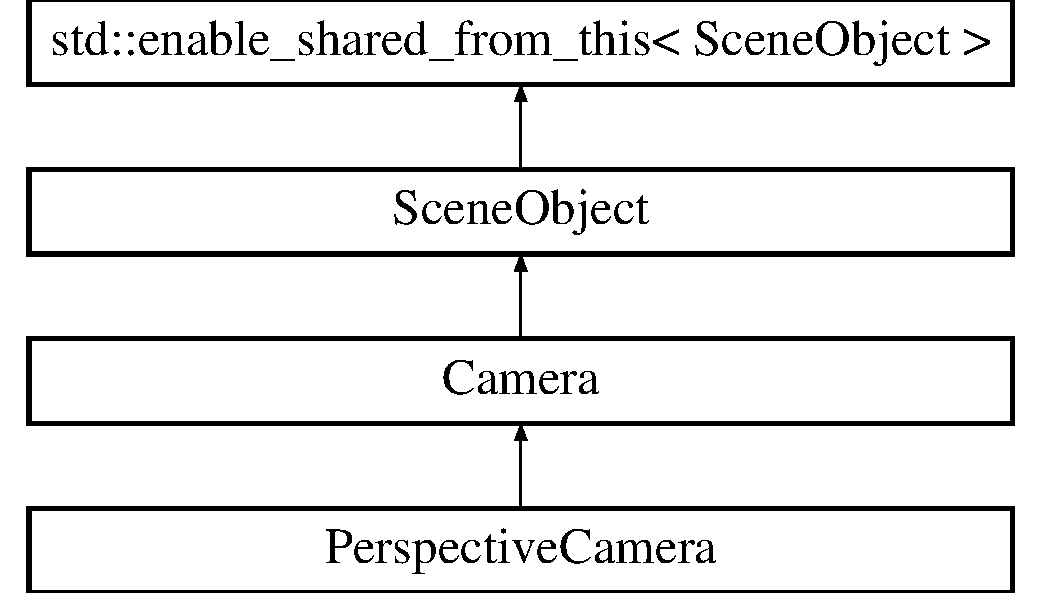
\includegraphics[height=4.000000cm]{class_perspective_camera}
\end{center}
\end{figure}
\subsection*{Public Member Functions}
\begin{DoxyCompactItemize}
\item 
\hypertarget{class_perspective_camera_adb5624bfee18c9390df3ba0612431124}{}{\bfseries Perspective\+Camera} (float in\+Fov, float in\+A\+R)\label{class_perspective_camera_adb5624bfee18c9390df3ba0612431124}

\item 
\hypertarget{class_perspective_camera_a24a338c552cede73ae7d69527ec85817}{}virtual glm\+::mat4 {\bfseries Get\+Projection\+Matrix} () const \label{class_perspective_camera_a24a338c552cede73ae7d69527ec85817}

\item 
\hypertarget{class_perspective_camera_a47ca1c9615ef9cb9dbe3436e561b76a0}{}virtual float {\bfseries Get\+F\+O\+V} () const \label{class_perspective_camera_a47ca1c9615ef9cb9dbe3436e561b76a0}

\item 
\hypertarget{class_perspective_camera_a03f2ce1c0940599712b12a07719b5122}{}virtual void {\bfseries Set\+F\+O\+V} (float in)\label{class_perspective_camera_a03f2ce1c0940599712b12a07719b5122}

\item 
\hypertarget{class_perspective_camera_a02d3e3a9a8b3770ed0cad810a3946dee}{}virtual float {\bfseries Get\+Aspect\+Ratio} () const \label{class_perspective_camera_a02d3e3a9a8b3770ed0cad810a3946dee}

\item 
\hypertarget{class_perspective_camera_a2f8753cd16d119ed00d050b4dbac2510}{}virtual void {\bfseries Set\+Aspect\+Ratio} (float in)\label{class_perspective_camera_a2f8753cd16d119ed00d050b4dbac2510}

\item 
\hypertarget{class_perspective_camera_a42fbe0fea96a362cd6e5e7e6414843ac}{}virtual float {\bfseries Get\+Z\+Near} () const \label{class_perspective_camera_a42fbe0fea96a362cd6e5e7e6414843ac}

\item 
\hypertarget{class_perspective_camera_ab9bab141c767e0b604b213f482f72c8a}{}virtual void {\bfseries Set\+Z\+Near} (float in)\label{class_perspective_camera_ab9bab141c767e0b604b213f482f72c8a}

\item 
\hypertarget{class_perspective_camera_a7e954166961c8d643c24fec0aa0261a4}{}virtual float {\bfseries Get\+Z\+Far} () const \label{class_perspective_camera_a7e954166961c8d643c24fec0aa0261a4}

\item 
\hypertarget{class_perspective_camera_a4374ca73880370dad1b93eaf489c9bb4}{}virtual void {\bfseries Set\+Z\+Far} (float in)\label{class_perspective_camera_a4374ca73880370dad1b93eaf489c9bb4}

\end{DoxyCompactItemize}
\subsection*{Protected Member Functions}
\begin{DoxyCompactItemize}
\item 
\hypertarget{class_perspective_camera_a2f17fb07425e2146d5692805753fa368}{}virtual void {\bfseries Update\+Transformation\+Matrix} ()\label{class_perspective_camera_a2f17fb07425e2146d5692805753fa368}

\end{DoxyCompactItemize}
\subsection*{Additional Inherited Members}


\subsection{Detailed Description}


Definition at line 8 of file Perspective\+Camera.\+h.



The documentation for this class was generated from the following files\+:\begin{DoxyCompactItemize}
\item 
/\+Users/michaelbao/workspace/cs148opengl4/source/common/\+Scene/\+Camera/Perspective\+Camera.\+h\item 
/\+Users/michaelbao/workspace/cs148opengl4/source/common/\+Scene/\+Camera/Perspective\+Camera.\+cpp\end{DoxyCompactItemize}

\hypertarget{class_renderer}{}\section{Renderer Class Reference}
\label{class_renderer}\index{Renderer@{Renderer}}


A generic rendering interface.  




{\ttfamily \#include $<$Renderer.\+h$>$}

Inheritance diagram for Renderer\+:\begin{figure}[H]
\begin{center}
\leavevmode
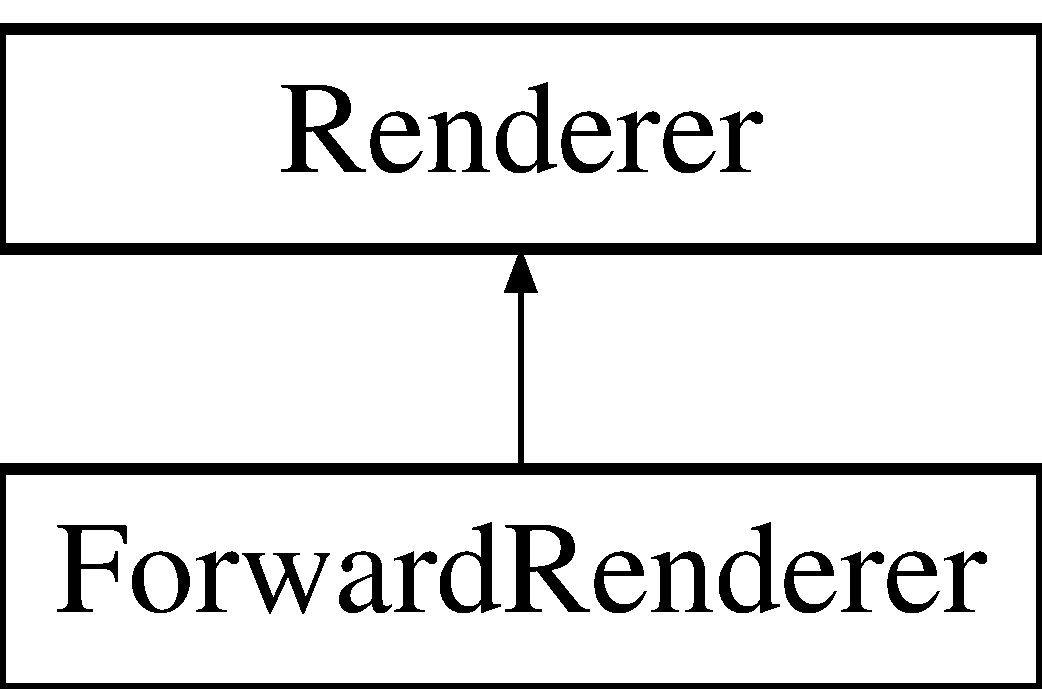
\includegraphics[height=2.000000cm]{class_renderer}
\end{center}
\end{figure}
\subsection*{Public Member Functions}
\begin{DoxyCompactItemize}
\item 
\hyperlink{class_renderer_adc8ce31cd649bdf220ca8355809b1d06}{Renderer} (std\+::shared\+\_\+ptr$<$ class \hyperlink{class_scene}{Scene} $>$ input\+Scene, std\+::shared\+\_\+ptr$<$ class \hyperlink{class_camera}{Camera} $>$ input\+Camera)
\begin{DoxyCompactList}\small\item\em The \hyperlink{class_renderer}{Renderer} constructor takes in a scene to be rendered and the camera from which to render the scene. \end{DoxyCompactList}\item 
virtual \hyperlink{class_renderer_afeee408862d5bd6255a6882d47e6d5cd}{$\sim$\+Renderer} ()
\begin{DoxyCompactList}\small\item\em A virtual destructor to allow for safe inheritance. \end{DoxyCompactList}\item 
virtual void \hyperlink{class_renderer_a7cb221f355f181d84d66e8c09f50f04a}{Initialize} ()=0
\begin{DoxyCompactList}\small\item\em Prepares the renderer for usage. \end{DoxyCompactList}\item 
virtual void \hyperlink{class_renderer_a38623da22aa718cfa41e2514ebd269f5}{Render} ()=0
\begin{DoxyCompactList}\small\item\em This function should be used to render everything onto the screen. \end{DoxyCompactList}\end{DoxyCompactItemize}
\subsection*{Protected Attributes}
\begin{DoxyCompactItemize}
\item 
std\+::shared\+\_\+ptr$<$ class \hyperlink{class_scene}{Scene} $>$ \hyperlink{class_renderer_a65178695d48824d3afd6fe40fd4915b6}{scene}
\begin{DoxyCompactList}\small\item\em Shared pointer to the scene. Should not be a null pointer when you go to render. \end{DoxyCompactList}\item 
std\+::shared\+\_\+ptr$<$ class \hyperlink{class_camera}{Camera} $>$ \hyperlink{class_renderer_a7a08c6489c1ffe8e346b9f205b4014ca}{camera}
\begin{DoxyCompactList}\small\item\em Shared pointer to the camera. Should not be a null pointer when you go to render. \end{DoxyCompactList}\end{DoxyCompactItemize}


\subsection{Detailed Description}
A generic rendering interface. 

The renderer will be used by the \hyperlink{class_media_layer}{Media\+Layer} and will be told to \hyperlink{class_renderer_a38623da22aa718cfa41e2514ebd269f5}{Render()} every frame. It is the renderer\textquotesingle{}s responsibility to make sure everything in the scene gets rendered properly with the right shader using all the lights. 

Definition at line 13 of file Renderer.\+h.



\subsection{Constructor \& Destructor Documentation}
\hypertarget{class_renderer_adc8ce31cd649bdf220ca8355809b1d06}{}\index{Renderer@{Renderer}!Renderer@{Renderer}}
\index{Renderer@{Renderer}!Renderer@{Renderer}}
\subsubsection[{Renderer}]{\setlength{\rightskip}{0pt plus 5cm}Renderer\+::\+Renderer (
\begin{DoxyParamCaption}
\item[{std\+::shared\+\_\+ptr$<$ class {\bf Scene} $>$}]{input\+Scene, }
\item[{std\+::shared\+\_\+ptr$<$ class {\bf Camera} $>$}]{input\+Camera}
\end{DoxyParamCaption}
)}\label{class_renderer_adc8ce31cd649bdf220ca8355809b1d06}


The \hyperlink{class_renderer}{Renderer} constructor takes in a scene to be rendered and the camera from which to render the scene. 


\begin{DoxyParams}{Parameters}
{\em input\+Scene} & A shared pointer to the scene. This can be a null pointer but you would need to introduce functions to set it later. \\
\hline
{\em input\+Camera} & A shared pointer to the camera. This can be a null pointer but you would need to introduce functions to set it later. \\
\hline
\end{DoxyParams}


Definition at line 6 of file Renderer.\+cpp.

\hypertarget{class_renderer_afeee408862d5bd6255a6882d47e6d5cd}{}\index{Renderer@{Renderer}!````~Renderer@{$\sim$\+Renderer}}
\index{````~Renderer@{$\sim$\+Renderer}!Renderer@{Renderer}}
\subsubsection[{$\sim$\+Renderer}]{\setlength{\rightskip}{0pt plus 5cm}Renderer\+::$\sim$\+Renderer (
\begin{DoxyParamCaption}
{}
\end{DoxyParamCaption}
)\hspace{0.3cm}{\ttfamily [virtual]}}\label{class_renderer_afeee408862d5bd6255a6882d47e6d5cd}


A virtual destructor to allow for safe inheritance. 



Definition at line 11 of file Renderer.\+cpp.



\subsection{Member Function Documentation}
\hypertarget{class_renderer_a7cb221f355f181d84d66e8c09f50f04a}{}\index{Renderer@{Renderer}!Initialize@{Initialize}}
\index{Initialize@{Initialize}!Renderer@{Renderer}}
\subsubsection[{Initialize}]{\setlength{\rightskip}{0pt plus 5cm}virtual void Renderer\+::\+Initialize (
\begin{DoxyParamCaption}
{}
\end{DoxyParamCaption}
)\hspace{0.3cm}{\ttfamily [pure virtual]}}\label{class_renderer_a7cb221f355f181d84d66e8c09f50f04a}


Prepares the renderer for usage. 

Called in the \hyperlink{class_media_layer}{Media\+Layer} constructor. 

Implemented in \hyperlink{class_forward_renderer_a99c523e11a4335d061da8bdba51f1c9a}{Forward\+Renderer}.

\hypertarget{class_renderer_a38623da22aa718cfa41e2514ebd269f5}{}\index{Renderer@{Renderer}!Render@{Render}}
\index{Render@{Render}!Renderer@{Renderer}}
\subsubsection[{Render}]{\setlength{\rightskip}{0pt plus 5cm}virtual void Renderer\+::\+Render (
\begin{DoxyParamCaption}
{}
\end{DoxyParamCaption}
)\hspace{0.3cm}{\ttfamily [pure virtual]}}\label{class_renderer_a38623da22aa718cfa41e2514ebd269f5}


This function should be used to render everything onto the screen. 



Implemented in \hyperlink{class_forward_renderer_a3693c5cd68afffc14652f24fcdc62abc}{Forward\+Renderer}.



\subsection{Member Data Documentation}
\hypertarget{class_renderer_a7a08c6489c1ffe8e346b9f205b4014ca}{}\index{Renderer@{Renderer}!camera@{camera}}
\index{camera@{camera}!Renderer@{Renderer}}
\subsubsection[{camera}]{\setlength{\rightskip}{0pt plus 5cm}std\+::shared\+\_\+ptr$<$class {\bf Camera}$>$ Renderer\+::camera\hspace{0.3cm}{\ttfamily [protected]}}\label{class_renderer_a7a08c6489c1ffe8e346b9f205b4014ca}


Shared pointer to the camera. Should not be a null pointer when you go to render. 



Definition at line 43 of file Renderer.\+h.

\hypertarget{class_renderer_a65178695d48824d3afd6fe40fd4915b6}{}\index{Renderer@{Renderer}!scene@{scene}}
\index{scene@{scene}!Renderer@{Renderer}}
\subsubsection[{scene}]{\setlength{\rightskip}{0pt plus 5cm}std\+::shared\+\_\+ptr$<$class {\bf Scene}$>$ Renderer\+::scene\hspace{0.3cm}{\ttfamily [protected]}}\label{class_renderer_a65178695d48824d3afd6fe40fd4915b6}


Shared pointer to the scene. Should not be a null pointer when you go to render. 



Definition at line 39 of file Renderer.\+h.



The documentation for this class was generated from the following files\+:\begin{DoxyCompactItemize}
\item 
/\+Users/michaelbao/workspace/cs148opengl4/source/common/\+Rendering/\hyperlink{_renderer_8h}{Renderer.\+h}\item 
/\+Users/michaelbao/workspace/cs148opengl4/source/common/\+Rendering/\hyperlink{_renderer_8cpp}{Renderer.\+cpp}\end{DoxyCompactItemize}

\hypertarget{class_rendering_object}{}\section{Rendering\+Object Class Reference}
\label{class_rendering_object}\index{Rendering\+Object@{Rendering\+Object}}


Stores the vertex data for a mesh.  




{\ttfamily \#include $<$Rendering\+Object.\+h$>$}

\subsection*{Public Types}
\begin{DoxyCompactItemize}
\item 
enum \hyperlink{class_rendering_object_ab772f569ef63a1db07db29a744b519ee}{Vertex\+Attribute\+Positions} \{ \hyperlink{class_rendering_object_ab772f569ef63a1db07db29a744b519eea52f5e0bc3859bc5f5e25130b6c7e8881}{Vertex\+Attribute\+Positions\+::\+Position} = 0, 
\hyperlink{class_rendering_object_ab772f569ef63a1db07db29a744b519eea4ab971a51f0335cbf8d9c2c65d379e99}{Vertex\+Attribute\+Positions\+::\+Normals}, 
\hyperlink{class_rendering_object_ab772f569ef63a1db07db29a744b519eeadeaa2adbeb26802ae61609c3f3642d82}{Vertex\+Attribute\+Positions\+::\+U\+V}, 
\hyperlink{class_rendering_object_ab772f569ef63a1db07db29a744b519eea5d50889672f6f860d14f502de3de1957}{Vertex\+Attribute\+Positions\+::\+Colors}
 \}
\begin{DoxyCompactList}\small\item\em This enum has its values corresponding to the layout location qualifer on the vertex attribute array. \end{DoxyCompactList}\item 
using \hyperlink{class_rendering_object_a1223b9cf03f2029b9c43d71042c2a18e}{Position\+Array} = std\+::vector$<$ glm\+::vec4 $>$
\item 
using \hyperlink{class_rendering_object_a9931c88bca3384065c6691dfe1e60af1}{Index\+Array} = std\+::vector$<$ unsigned int $>$
\item 
using \hyperlink{class_rendering_object_a327c4d892de8d6138fb59afa6d078257}{Normal\+Array} = std\+::vector$<$ glm\+::vec3 $>$
\item 
using \hyperlink{class_rendering_object_a504ecd45ebe36dfa5b78c46d64d9904a}{U\+V\+Array} = std\+::vector$<$ glm\+::vec2 $>$
\item 
using \hyperlink{class_rendering_object_a8a12e1f9be788d99af6c089e1c600022}{Color\+Array} = std\+::vector$<$ glm\+::vec4 $>$
\end{DoxyCompactItemize}
\subsection*{Public Member Functions}
\begin{DoxyCompactItemize}
\item 
\hyperlink{class_rendering_object_a0550d86d49a01032921150d1c09c378f}{Rendering\+Object} (std\+::shared\+\_\+ptr$<$ class \hyperlink{class_shader_program}{Shader\+Program} $>$ input\+Shader, std\+::unique\+\_\+ptr$<$ \hyperlink{class_rendering_object_a1223b9cf03f2029b9c43d71042c2a18e}{Position\+Array} $>$ input\+Positions, std\+::unique\+\_\+ptr$<$ \hyperlink{class_rendering_object_a9931c88bca3384065c6691dfe1e60af1}{Index\+Array} $>$ input\+Indices=nullptr, std\+::unique\+\_\+ptr$<$ \hyperlink{class_rendering_object_a327c4d892de8d6138fb59afa6d078257}{Normal\+Array} $>$ input\+Normals=nullptr, std\+::unique\+\_\+ptr$<$ \hyperlink{class_rendering_object_a504ecd45ebe36dfa5b78c46d64d9904a}{U\+V\+Array} $>$ input\+U\+V=nullptr, std\+::unique\+\_\+ptr$<$ \hyperlink{class_rendering_object_a8a12e1f9be788d99af6c089e1c600022}{Color\+Array} $>$ input\+Colors=nullptr)
\begin{DoxyCompactList}\small\item\em Constructs a \hyperlink{class_rendering_object}{Rendering\+Object} from a shader and all the possible vertex attributes. \end{DoxyCompactList}\item 
virtual \hyperlink{class_rendering_object_ae4e8e14104ee3a587d10c9f90ec82048}{$\sim$\+Rendering\+Object} ()
\begin{DoxyCompactList}\small\item\em Just another deconstructor. \end{DoxyCompactList}\item 
virtual void \hyperlink{class_rendering_object_a22311d08bb7559f6b913afe314a5031e}{Set\+Shader} (std\+::shared\+\_\+ptr$<$ class \hyperlink{class_shader_program}{Shader\+Program} $>$ input\+Shader)
\begin{DoxyCompactList}\small\item\em Sets the shader to be used to render this object. \end{DoxyCompactList}\item 
virtual void \hyperlink{class_rendering_object_afa4510ba81fb7b17b940c92b27442d93}{Begin\+Render} () const 
\begin{DoxyCompactList}\small\item\em Prepares to the mesh object. \end{DoxyCompactList}\item 
virtual void \hyperlink{class_rendering_object_a5fdb7a1b2d53b7ce024a4eeabd9c86d3}{Render} () const 
\begin{DoxyCompactList}\small\item\em Calls the appropriate draw function depending on whether or not an element buffer object is used. \end{DoxyCompactList}\item 
virtual void \hyperlink{class_rendering_object_a2a038472f934360acddd26f4e992b28b}{End\+Render} () const 
\begin{DoxyCompactList}\small\item\em Unbinds the V\+A\+O and the E\+B\+O to cleanup the state. \end{DoxyCompactList}\item 
void \hyperlink{class_rendering_object_aa627eb310f11d0e04dbbb3665f58bb4e}{Set\+Draw\+Mode} (G\+Lenum input\+Mode)
\begin{DoxyCompactList}\small\item\em Sets what kind of primitives Open\+G\+L should interpret the data as. \end{DoxyCompactList}\item 
G\+Lint \hyperlink{class_rendering_object_a80658debd2668b55a3c9fe86ec9f49fb}{Get\+Shader\+Program} () const 
\begin{DoxyCompactList}\small\item\em Returns the Open\+G\+L identifier for the underlying shader program. \end{DoxyCompactList}\item 
const class \hyperlink{class_shader_program}{Shader\+Program} $\ast$ \hyperlink{class_rendering_object_ac9187166c98131aab185111e105528c2}{Get\+Shader\+Program\+Raw} () const 
\begin{DoxyCompactList}\small\item\em Returns a raw pointer to the underlying shader program. \end{DoxyCompactList}\item 
size\+\_\+t \hyperlink{class_rendering_object_a3bb36683836c8c177984aa928cb1fb04}{Get\+Total\+Vertices} () const 
\begin{DoxyCompactList}\small\item\em Returns the total number of vertices. \end{DoxyCompactList}\item 
virtual void \hyperlink{class_rendering_object_ada51886b7da1924a17d3a55e8fe90061}{Set\+Vertex\+Positions} (std\+::unique\+\_\+ptr$<$ \hyperlink{class_rendering_object_a1223b9cf03f2029b9c43d71042c2a18e}{Position\+Array} $>$ positions)
\begin{DoxyCompactList}\small\item\em Sets the vertex positions array. Also updates the data stored in the vertex buffer object. \end{DoxyCompactList}\item 
virtual void \hyperlink{class_rendering_object_a61ea597df0c456834eac8eb4087fb573}{Set\+Vertex\+Indices} (std\+::unique\+\_\+ptr$<$ \hyperlink{class_rendering_object_a9931c88bca3384065c6691dfe1e60af1}{Index\+Array} $>$ indices)
\begin{DoxyCompactList}\small\item\em Sets the vertex indices array. Also updates the data stored in the element buffer object. \end{DoxyCompactList}\item 
virtual void \hyperlink{class_rendering_object_a4cd085aed01fbc5e4fae7076e00919d3}{Set\+Vertex\+Normals} (std\+::unique\+\_\+ptr$<$ \hyperlink{class_rendering_object_a327c4d892de8d6138fb59afa6d078257}{Normal\+Array} $>$ normals)
\begin{DoxyCompactList}\small\item\em Sets the vertex normal array. Also updates the data stored in the vertex buffer object. \end{DoxyCompactList}\item 
virtual void \hyperlink{class_rendering_object_a2a2b3c6ec2d13e8d3a4b6ac4c05ae11b}{Set\+Vertex\+U\+V} (std\+::unique\+\_\+ptr$<$ \hyperlink{class_rendering_object_a504ecd45ebe36dfa5b78c46d64d9904a}{U\+V\+Array} $>$ uv)
\begin{DoxyCompactList}\small\item\em Sets the vertex U\+V array. Also updates the data stored in the vertex buffer object. \end{DoxyCompactList}\item 
virtual void \hyperlink{class_rendering_object_aa1170c47ff02b2305a54c8aab3460201}{Set\+Vertex\+Colors} (std\+::unique\+\_\+ptr$<$ \hyperlink{class_rendering_object_a8a12e1f9be788d99af6c089e1c600022}{Color\+Array} $>$ colors)
\begin{DoxyCompactList}\small\item\em Sets the vertex color array. Also updates the data stored in the vertex buffer object. \end{DoxyCompactList}\end{DoxyCompactItemize}
\subsection*{Protected Member Functions}
\begin{DoxyCompactItemize}
\item 
virtual void \hyperlink{class_rendering_object_a77c78d1b42ea2ebfdbf994b6b91ce805}{Initialize\+Open\+G\+L} ()
\begin{DoxyCompactList}\small\item\em Prepares the rendering object for use by Open\+G\+L. \end{DoxyCompactList}\item 
virtual void \hyperlink{class_rendering_object_a7a097727acf37f9671ddd5e3a9873771}{Update\+Vertex\+Positions} ()
\item 
virtual void \hyperlink{class_rendering_object_afb49054121b1b552bce58625db91b851}{Update\+Vertex\+Indices} ()
\item 
virtual void \hyperlink{class_rendering_object_ae4b537e1c9b1c5c50cb7b0db83e6f190}{Update\+Vertex\+Normals} ()
\item 
virtual void \hyperlink{class_rendering_object_ac00889f2afaa605b09164649ef68a1b6}{Update\+Vertex\+U\+V} ()
\item 
virtual void \hyperlink{class_rendering_object_aca18dbb9252f27cef09df307dbcf02a9}{Update\+Vertex\+Colors} ()
\item 
virtual void \hyperlink{class_rendering_object_af9c1a07398071cdd0cca3ad36095fc85}{Cleanup\+Vertex\+Positions} ()
\item 
virtual void \hyperlink{class_rendering_object_ac60c8a7f3d5678fd4aa8198f6c980e6e}{Cleanup\+Vertex\+Indices} ()
\item 
virtual void \hyperlink{class_rendering_object_ad89bc24893f8fe32794f0686c2bb0da1}{Cleanup\+Vertex\+Normals} ()
\item 
virtual void \hyperlink{class_rendering_object_a776f54b41f9e9f0e55fc1104919c3e7c}{Cleanup\+Vertex\+U\+V} ()
\item 
virtual void \hyperlink{class_rendering_object_adce4a6d6406eb589b088bedd19127f32}{Cleanup\+Vertex\+Colors} ()
\end{DoxyCompactItemize}
\subsection*{Protected Attributes}
\begin{DoxyCompactItemize}
\item 
std\+::shared\+\_\+ptr$<$ class \hyperlink{class_shader_program}{Shader\+Program} $>$ \hyperlink{class_rendering_object_ae50e545ce2008ffa802478cd4316e82e}{shader}
\begin{DoxyCompactList}\small\item\em The shader program used to render the object. \end{DoxyCompactList}\item 
G\+Luint \hyperlink{class_rendering_object_a473f623b39157288bef992e76ddc45a9}{vertex\+Position\+Buffer}
\begin{DoxyCompactList}\small\item\em The buffer I\+D for the vertex position V\+B\+O as generated by \href{https://www.opengl.org/sdk/docs/man/html/glGenBuffers.xhtml}{\tt gl\+Gen\+Buffers}. \end{DoxyCompactList}\item 
std\+::unique\+\_\+ptr$<$ \hyperlink{class_rendering_object_a1223b9cf03f2029b9c43d71042c2a18e}{Position\+Array} $>$ \hyperlink{class_rendering_object_a14721712672d0421ed72a394e3131da0}{vertex\+Positions}
\begin{DoxyCompactList}\small\item\em The position of every vertex. \end{DoxyCompactList}\item 
G\+Luint \hyperlink{class_rendering_object_a6740a0a0e6bd4d841c9c211f2a31cca3}{vertex\+Index\+Buffer}
\begin{DoxyCompactList}\small\item\em The buffer I\+D for the vertex index E\+B\+O as generated by \href{https://www.opengl.org/sdk/docs/man/html/glGenBuffers.xhtml}{\tt gl\+Gen\+Buffers}. \end{DoxyCompactList}\item 
std\+::unique\+\_\+ptr$<$ \hyperlink{class_rendering_object_a9931c88bca3384065c6691dfe1e60af1}{Index\+Array} $>$ \hyperlink{class_rendering_object_a7b84487d3c34c1ca36b2ac6060b0f802}{vertex\+Indices}
\begin{DoxyCompactList}\small\item\em The indices into the vertex array. This allows us to reuse vertices for multiple faces. \end{DoxyCompactList}\item 
G\+Luint \hyperlink{class_rendering_object_a91649e3a653f2266cd00c718f10849f9}{vertex\+Normal\+Buffer}
\begin{DoxyCompactList}\small\item\em The buffer I\+D for the vertex normal V\+B\+O as generated by \href{https://www.opengl.org/sdk/docs/man/html/glGenBuffers.xhtml}{\tt gl\+Gen\+Buffers}. \end{DoxyCompactList}\item 
std\+::unique\+\_\+ptr$<$ \hyperlink{class_rendering_object_a327c4d892de8d6138fb59afa6d078257}{Normal\+Array} $>$ \hyperlink{class_rendering_object_ac28d301f97d29ab603f65f8e823063b4}{vertex\+Normals}
\begin{DoxyCompactList}\small\item\em The normal of every vertex. \end{DoxyCompactList}\item 
G\+Luint \hyperlink{class_rendering_object_ad583c70014e3f6ab0c9b62ea3c96ad25}{vertex\+U\+V\+Buffer}
\begin{DoxyCompactList}\small\item\em The buffer I\+D for the vertex U\+V V\+B\+O as generated by \href{https://www.opengl.org/sdk/docs/man/html/glGenBuffers.xhtml}{\tt gl\+Gen\+Buffers}. \end{DoxyCompactList}\item 
std\+::unique\+\_\+ptr$<$ \hyperlink{class_rendering_object_a504ecd45ebe36dfa5b78c46d64d9904a}{U\+V\+Array} $>$ \hyperlink{class_rendering_object_afc405316bddec4ba1d5c228ecc0d9061}{vertex\+U\+V}
\begin{DoxyCompactList}\small\item\em The U\+V coordinate of every vertex. \end{DoxyCompactList}\item 
G\+Luint \hyperlink{class_rendering_object_aeb014a4ef24e2fc4665a769241660cad}{vertex\+Color\+Buffer}
\begin{DoxyCompactList}\small\item\em The buffer I\+D for the vertex color V\+B\+O as generated by \href{https://www.opengl.org/sdk/docs/man/html/glGenBuffers.xhtml}{\tt gl\+Gen\+Buffers}. \end{DoxyCompactList}\item 
std\+::unique\+\_\+ptr$<$ \hyperlink{class_rendering_object_a8a12e1f9be788d99af6c089e1c600022}{Color\+Array} $>$ \hyperlink{class_rendering_object_a65fc52e665791ce55e43106b603e917a}{vertex\+Colors}
\begin{DoxyCompactList}\small\item\em The color of every vertex. \end{DoxyCompactList}\item 
G\+Luint \hyperlink{class_rendering_object_a96dd05670a977a949514a2c490c1c867}{vao}
\item 
G\+Lenum \hyperlink{class_rendering_object_aa67856a72705b54a5667e91e270d00b3}{draw\+Mode}
\end{DoxyCompactItemize}
\subsection*{Static Protected Attributes}
\begin{DoxyCompactItemize}
\item 
static glm\+::vec3 \hyperlink{class_rendering_object_af270a476ba12c23fefbb034e21930add}{D\+E\+F\+A\+U\+L\+T\+\_\+\+N\+O\+R\+M\+A\+L}
\begin{DoxyCompactList}\small\item\em The default value sent to the shader if \hyperlink{class_rendering_object_ac28d301f97d29ab603f65f8e823063b4}{Rendering\+Object\+::vertex\+Normals} is not set. \end{DoxyCompactList}\item 
static glm\+::vec2 \hyperlink{class_rendering_object_a3dcb28a12f578630aea75cc59ea39588}{D\+E\+F\+A\+U\+L\+T\+\_\+\+U\+V}
\begin{DoxyCompactList}\small\item\em The default value sent to the shader if \hyperlink{class_rendering_object_afc405316bddec4ba1d5c228ecc0d9061}{Rendering\+Object\+::vertex\+U\+V} is not set. \end{DoxyCompactList}\item 
static glm\+::vec4 \hyperlink{class_rendering_object_a3bf21996dc0ef604b2b81d95275c97f9}{D\+E\+F\+A\+U\+L\+T\+\_\+\+C\+O\+L\+O\+R}
\begin{DoxyCompactList}\small\item\em The default value sent to the shader if \hyperlink{class_rendering_object_a65fc52e665791ce55e43106b603e917a}{Rendering\+Object\+::vertex\+Colors} is not set. \end{DoxyCompactList}\end{DoxyCompactItemize}


\subsection{Detailed Description}
Stores the vertex data for a mesh. 

This class allows us to easily reuse the same mesh data for multiple objects in the scene. 

Definition at line 13 of file Rendering\+Object.\+h.



\subsection{Member Typedef Documentation}
\hypertarget{class_rendering_object_a8a12e1f9be788d99af6c089e1c600022}{}\index{Rendering\+Object@{Rendering\+Object}!Color\+Array@{Color\+Array}}
\index{Color\+Array@{Color\+Array}!Rendering\+Object@{Rendering\+Object}}
\subsubsection[{Color\+Array}]{\setlength{\rightskip}{0pt plus 5cm}using {\bf Rendering\+Object\+::\+Color\+Array} =  std\+::vector$<$glm\+::vec4$>$}\label{class_rendering_object_a8a12e1f9be788d99af6c089e1c600022}


Definition at line 20 of file Rendering\+Object.\+h.

\hypertarget{class_rendering_object_a9931c88bca3384065c6691dfe1e60af1}{}\index{Rendering\+Object@{Rendering\+Object}!Index\+Array@{Index\+Array}}
\index{Index\+Array@{Index\+Array}!Rendering\+Object@{Rendering\+Object}}
\subsubsection[{Index\+Array}]{\setlength{\rightskip}{0pt plus 5cm}using {\bf Rendering\+Object\+::\+Index\+Array} =  std\+::vector$<$unsigned int$>$}\label{class_rendering_object_a9931c88bca3384065c6691dfe1e60af1}


Definition at line 17 of file Rendering\+Object.\+h.

\hypertarget{class_rendering_object_a327c4d892de8d6138fb59afa6d078257}{}\index{Rendering\+Object@{Rendering\+Object}!Normal\+Array@{Normal\+Array}}
\index{Normal\+Array@{Normal\+Array}!Rendering\+Object@{Rendering\+Object}}
\subsubsection[{Normal\+Array}]{\setlength{\rightskip}{0pt plus 5cm}using {\bf Rendering\+Object\+::\+Normal\+Array} =  std\+::vector$<$glm\+::vec3$>$}\label{class_rendering_object_a327c4d892de8d6138fb59afa6d078257}


Definition at line 18 of file Rendering\+Object.\+h.

\hypertarget{class_rendering_object_a1223b9cf03f2029b9c43d71042c2a18e}{}\index{Rendering\+Object@{Rendering\+Object}!Position\+Array@{Position\+Array}}
\index{Position\+Array@{Position\+Array}!Rendering\+Object@{Rendering\+Object}}
\subsubsection[{Position\+Array}]{\setlength{\rightskip}{0pt plus 5cm}using {\bf Rendering\+Object\+::\+Position\+Array} =  std\+::vector$<$glm\+::vec4$>$}\label{class_rendering_object_a1223b9cf03f2029b9c43d71042c2a18e}


Definition at line 16 of file Rendering\+Object.\+h.

\hypertarget{class_rendering_object_a504ecd45ebe36dfa5b78c46d64d9904a}{}\index{Rendering\+Object@{Rendering\+Object}!U\+V\+Array@{U\+V\+Array}}
\index{U\+V\+Array@{U\+V\+Array}!Rendering\+Object@{Rendering\+Object}}
\subsubsection[{U\+V\+Array}]{\setlength{\rightskip}{0pt plus 5cm}using {\bf Rendering\+Object\+::\+U\+V\+Array} =  std\+::vector$<$glm\+::vec2$>$}\label{class_rendering_object_a504ecd45ebe36dfa5b78c46d64d9904a}


Definition at line 19 of file Rendering\+Object.\+h.



\subsection{Member Enumeration Documentation}
\hypertarget{class_rendering_object_ab772f569ef63a1db07db29a744b519ee}{}\index{Rendering\+Object@{Rendering\+Object}!Vertex\+Attribute\+Positions@{Vertex\+Attribute\+Positions}}
\index{Vertex\+Attribute\+Positions@{Vertex\+Attribute\+Positions}!Rendering\+Object@{Rendering\+Object}}
\subsubsection[{Vertex\+Attribute\+Positions}]{\setlength{\rightskip}{0pt plus 5cm}enum {\bf Rendering\+Object\+::\+Vertex\+Attribute\+Positions}\hspace{0.3cm}{\ttfamily [strong]}}\label{class_rendering_object_ab772f569ef63a1db07db29a744b519ee}


This enum has its values corresponding to the layout location qualifer on the vertex attribute array. 

\begin{Desc}
\item[Enumerator]\par
\begin{description}
\index{Position@{Position}!Rendering\+Object@{Rendering\+Object}}\index{Rendering\+Object@{Rendering\+Object}!Position@{Position}}\item[{\em 
\hypertarget{class_rendering_object_ab772f569ef63a1db07db29a744b519eea52f5e0bc3859bc5f5e25130b6c7e8881}{}Position\label{class_rendering_object_ab772f569ef63a1db07db29a744b519eea52f5e0bc3859bc5f5e25130b6c7e8881}
}]\index{Normals@{Normals}!Rendering\+Object@{Rendering\+Object}}\index{Rendering\+Object@{Rendering\+Object}!Normals@{Normals}}\item[{\em 
\hypertarget{class_rendering_object_ab772f569ef63a1db07db29a744b519eea4ab971a51f0335cbf8d9c2c65d379e99}{}Normals\label{class_rendering_object_ab772f569ef63a1db07db29a744b519eea4ab971a51f0335cbf8d9c2c65d379e99}
}]\index{U\+V@{U\+V}!Rendering\+Object@{Rendering\+Object}}\index{Rendering\+Object@{Rendering\+Object}!U\+V@{U\+V}}\item[{\em 
\hypertarget{class_rendering_object_ab772f569ef63a1db07db29a744b519eeadeaa2adbeb26802ae61609c3f3642d82}{}U\+V\label{class_rendering_object_ab772f569ef63a1db07db29a744b519eeadeaa2adbeb26802ae61609c3f3642d82}
}]\index{Colors@{Colors}!Rendering\+Object@{Rendering\+Object}}\index{Rendering\+Object@{Rendering\+Object}!Colors@{Colors}}\item[{\em 
\hypertarget{class_rendering_object_ab772f569ef63a1db07db29a744b519eea5d50889672f6f860d14f502de3de1957}{}Colors\label{class_rendering_object_ab772f569ef63a1db07db29a744b519eea5d50889672f6f860d14f502de3de1957}
}]\end{description}
\end{Desc}


Definition at line 24 of file Rendering\+Object.\+h.



\subsection{Constructor \& Destructor Documentation}
\hypertarget{class_rendering_object_a0550d86d49a01032921150d1c09c378f}{}\index{Rendering\+Object@{Rendering\+Object}!Rendering\+Object@{Rendering\+Object}}
\index{Rendering\+Object@{Rendering\+Object}!Rendering\+Object@{Rendering\+Object}}
\subsubsection[{Rendering\+Object}]{\setlength{\rightskip}{0pt plus 5cm}Rendering\+Object\+::\+Rendering\+Object (
\begin{DoxyParamCaption}
\item[{std\+::shared\+\_\+ptr$<$ class {\bf Shader\+Program} $>$}]{input\+Shader, }
\item[{std\+::unique\+\_\+ptr$<$ {\bf Position\+Array} $>$}]{input\+Positions, }
\item[{std\+::unique\+\_\+ptr$<$ {\bf Index\+Array} $>$}]{input\+Indices = {\ttfamily nullptr}, }
\item[{std\+::unique\+\_\+ptr$<$ {\bf Normal\+Array} $>$}]{input\+Normals = {\ttfamily nullptr}, }
\item[{std\+::unique\+\_\+ptr$<$ {\bf U\+V\+Array} $>$}]{input\+U\+V = {\ttfamily nullptr}, }
\item[{std\+::unique\+\_\+ptr$<$ {\bf Color\+Array} $>$}]{input\+Colors = {\ttfamily nullptr}}
\end{DoxyParamCaption}
)}\label{class_rendering_object_a0550d86d49a01032921150d1c09c378f}


Constructs a \hyperlink{class_rendering_object}{Rendering\+Object} from a shader and all the possible vertex attributes. 


\begin{DoxyParams}{Parameters}
{\em input\+Shader} & The shader that is to be used to render this object. Can be a nullptr and set later. \\
\hline
{\em input\+Positions} & The vertex positions. Should not be a null pointer (you can probably get away with it and set it later...). \\
\hline
{\em input\+Normals} & The vertex normals. Can be set later. \\
\hline
{\em input\+U\+V} & The vertex U\+V coordinates. Can be set later. \\
\hline
{\em input\+Colors} & The vertex colors. Can be set later.\\
\hline
\end{DoxyParams}
Constructs a new object that holds the data necessary to render an object. Note that the ordering of the vertex attributes is the same regardless of whether or not the vertex attribute array is actually used by the shader. In other words, vertex U\+V\textquotesingle{}s will always be at location 2 regardless of whether the vertex normals are set and/or used. Once the \hyperlink{class_rendering_object}{Rendering\+Object} is created, the Open\+G\+L V\+B\+O\textquotesingle{}s and V\+A\+O\textquotesingle{}s will be constructed and all available data will be copied into the Open\+G\+L buffer. 

Definition at line 8 of file Rendering\+Object.\+cpp.

\hypertarget{class_rendering_object_ae4e8e14104ee3a587d10c9f90ec82048}{}\index{Rendering\+Object@{Rendering\+Object}!````~Rendering\+Object@{$\sim$\+Rendering\+Object}}
\index{````~Rendering\+Object@{$\sim$\+Rendering\+Object}!Rendering\+Object@{Rendering\+Object}}
\subsubsection[{$\sim$\+Rendering\+Object}]{\setlength{\rightskip}{0pt plus 5cm}Rendering\+Object\+::$\sim$\+Rendering\+Object (
\begin{DoxyParamCaption}
{}
\end{DoxyParamCaption}
)\hspace{0.3cm}{\ttfamily [virtual]}}\label{class_rendering_object_ae4e8e14104ee3a587d10c9f90ec82048}


Just another deconstructor. 



Definition at line 26 of file Rendering\+Object.\+cpp.



\subsection{Member Function Documentation}
\hypertarget{class_rendering_object_afa4510ba81fb7b17b940c92b27442d93}{}\index{Rendering\+Object@{Rendering\+Object}!Begin\+Render@{Begin\+Render}}
\index{Begin\+Render@{Begin\+Render}!Rendering\+Object@{Rendering\+Object}}
\subsubsection[{Begin\+Render}]{\setlength{\rightskip}{0pt plus 5cm}void Rendering\+Object\+::\+Begin\+Render (
\begin{DoxyParamCaption}
{}
\end{DoxyParamCaption}
) const\hspace{0.3cm}{\ttfamily [virtual]}}\label{class_rendering_object_afa4510ba81fb7b17b940c92b27442d93}


Prepares to the mesh object. 

We bind the vertex array object using \href{https://www.opengl.org/sdk/docs/man/html/glBindVertexArray.xhtml}{\tt gl\+Bind\+Vertex\+Array} and the element buffer object so that Open\+G\+L knows what to render. 

Definition at line 54 of file Rendering\+Object.\+cpp.

\hypertarget{class_rendering_object_adce4a6d6406eb589b088bedd19127f32}{}\index{Rendering\+Object@{Rendering\+Object}!Cleanup\+Vertex\+Colors@{Cleanup\+Vertex\+Colors}}
\index{Cleanup\+Vertex\+Colors@{Cleanup\+Vertex\+Colors}!Rendering\+Object@{Rendering\+Object}}
\subsubsection[{Cleanup\+Vertex\+Colors}]{\setlength{\rightskip}{0pt plus 5cm}void Rendering\+Object\+::\+Cleanup\+Vertex\+Colors (
\begin{DoxyParamCaption}
{}
\end{DoxyParamCaption}
)\hspace{0.3cm}{\ttfamily [protected]}, {\ttfamily [virtual]}}\label{class_rendering_object_adce4a6d6406eb589b088bedd19127f32}


Definition at line 258 of file Rendering\+Object.\+cpp.

\hypertarget{class_rendering_object_ac60c8a7f3d5678fd4aa8198f6c980e6e}{}\index{Rendering\+Object@{Rendering\+Object}!Cleanup\+Vertex\+Indices@{Cleanup\+Vertex\+Indices}}
\index{Cleanup\+Vertex\+Indices@{Cleanup\+Vertex\+Indices}!Rendering\+Object@{Rendering\+Object}}
\subsubsection[{Cleanup\+Vertex\+Indices}]{\setlength{\rightskip}{0pt plus 5cm}void Rendering\+Object\+::\+Cleanup\+Vertex\+Indices (
\begin{DoxyParamCaption}
{}
\end{DoxyParamCaption}
)\hspace{0.3cm}{\ttfamily [protected]}, {\ttfamily [virtual]}}\label{class_rendering_object_ac60c8a7f3d5678fd4aa8198f6c980e6e}


Definition at line 240 of file Rendering\+Object.\+cpp.

\hypertarget{class_rendering_object_ad89bc24893f8fe32794f0686c2bb0da1}{}\index{Rendering\+Object@{Rendering\+Object}!Cleanup\+Vertex\+Normals@{Cleanup\+Vertex\+Normals}}
\index{Cleanup\+Vertex\+Normals@{Cleanup\+Vertex\+Normals}!Rendering\+Object@{Rendering\+Object}}
\subsubsection[{Cleanup\+Vertex\+Normals}]{\setlength{\rightskip}{0pt plus 5cm}void Rendering\+Object\+::\+Cleanup\+Vertex\+Normals (
\begin{DoxyParamCaption}
{}
\end{DoxyParamCaption}
)\hspace{0.3cm}{\ttfamily [protected]}, {\ttfamily [virtual]}}\label{class_rendering_object_ad89bc24893f8fe32794f0686c2bb0da1}


Definition at line 246 of file Rendering\+Object.\+cpp.

\hypertarget{class_rendering_object_af9c1a07398071cdd0cca3ad36095fc85}{}\index{Rendering\+Object@{Rendering\+Object}!Cleanup\+Vertex\+Positions@{Cleanup\+Vertex\+Positions}}
\index{Cleanup\+Vertex\+Positions@{Cleanup\+Vertex\+Positions}!Rendering\+Object@{Rendering\+Object}}
\subsubsection[{Cleanup\+Vertex\+Positions}]{\setlength{\rightskip}{0pt plus 5cm}void Rendering\+Object\+::\+Cleanup\+Vertex\+Positions (
\begin{DoxyParamCaption}
{}
\end{DoxyParamCaption}
)\hspace{0.3cm}{\ttfamily [protected]}, {\ttfamily [virtual]}}\label{class_rendering_object_af9c1a07398071cdd0cca3ad36095fc85}


Definition at line 234 of file Rendering\+Object.\+cpp.

\hypertarget{class_rendering_object_a776f54b41f9e9f0e55fc1104919c3e7c}{}\index{Rendering\+Object@{Rendering\+Object}!Cleanup\+Vertex\+U\+V@{Cleanup\+Vertex\+U\+V}}
\index{Cleanup\+Vertex\+U\+V@{Cleanup\+Vertex\+U\+V}!Rendering\+Object@{Rendering\+Object}}
\subsubsection[{Cleanup\+Vertex\+U\+V}]{\setlength{\rightskip}{0pt plus 5cm}void Rendering\+Object\+::\+Cleanup\+Vertex\+U\+V (
\begin{DoxyParamCaption}
{}
\end{DoxyParamCaption}
)\hspace{0.3cm}{\ttfamily [protected]}, {\ttfamily [virtual]}}\label{class_rendering_object_a776f54b41f9e9f0e55fc1104919c3e7c}


Definition at line 252 of file Rendering\+Object.\+cpp.

\hypertarget{class_rendering_object_a2a038472f934360acddd26f4e992b28b}{}\index{Rendering\+Object@{Rendering\+Object}!End\+Render@{End\+Render}}
\index{End\+Render@{End\+Render}!Rendering\+Object@{Rendering\+Object}}
\subsubsection[{End\+Render}]{\setlength{\rightskip}{0pt plus 5cm}void Rendering\+Object\+::\+End\+Render (
\begin{DoxyParamCaption}
{}
\end{DoxyParamCaption}
) const\hspace{0.3cm}{\ttfamily [virtual]}}\label{class_rendering_object_a2a038472f934360acddd26f4e992b28b}


Unbinds the V\+A\+O and the E\+B\+O to cleanup the state. 



Definition at line 73 of file Rendering\+Object.\+cpp.

\hypertarget{class_rendering_object_a80658debd2668b55a3c9fe86ec9f49fb}{}\index{Rendering\+Object@{Rendering\+Object}!Get\+Shader\+Program@{Get\+Shader\+Program}}
\index{Get\+Shader\+Program@{Get\+Shader\+Program}!Rendering\+Object@{Rendering\+Object}}
\subsubsection[{Get\+Shader\+Program}]{\setlength{\rightskip}{0pt plus 5cm}G\+Lint Rendering\+Object\+::\+Get\+Shader\+Program (
\begin{DoxyParamCaption}
{}
\end{DoxyParamCaption}
) const}\label{class_rendering_object_a80658debd2668b55a3c9fe86ec9f49fb}


Returns the Open\+G\+L identifier for the underlying shader program. 

\begin{DoxyReturn}{Returns}
Returns the value that was generated by \href{https://www.opengl.org/sdk/docs/man/html/glCreateProgram.xhtml}{\tt gl\+Create\+Program} for the underlying shader program. 
\end{DoxyReturn}
\begin{DoxyWarning}{Warning}
If \hyperlink{class_rendering_object_ae50e545ce2008ffa802478cd4316e82e}{Rendering\+Object\+::shader} is not set to a non-\/null pointer, this function\textquotesingle{}s action is undefined. 
\end{DoxyWarning}


Definition at line 79 of file Rendering\+Object.\+cpp.

\hypertarget{class_rendering_object_ac9187166c98131aab185111e105528c2}{}\index{Rendering\+Object@{Rendering\+Object}!Get\+Shader\+Program\+Raw@{Get\+Shader\+Program\+Raw}}
\index{Get\+Shader\+Program\+Raw@{Get\+Shader\+Program\+Raw}!Rendering\+Object@{Rendering\+Object}}
\subsubsection[{Get\+Shader\+Program\+Raw}]{\setlength{\rightskip}{0pt plus 5cm}const {\bf Shader\+Program} $\ast$ Rendering\+Object\+::\+Get\+Shader\+Program\+Raw (
\begin{DoxyParamCaption}
{}
\end{DoxyParamCaption}
) const}\label{class_rendering_object_ac9187166c98131aab185111e105528c2}


Returns a raw pointer to the underlying shader program. 

\begin{DoxyReturn}{Returns}
Returns a raw pointer to the underlying shader program. 
\end{DoxyReturn}
\begin{DoxyWarning}{Warning}
If \hyperlink{class_rendering_object_ae50e545ce2008ffa802478cd4316e82e}{Rendering\+Object\+::shader} is not set to a non-\/null pointer, this function\textquotesingle{}s action is undefined. 

Do not store the \hyperlink{class_shader_program}{Shader\+Program} pointer anywhere. You may be left with a dangling pointer at some point. 
\end{DoxyWarning}


Definition at line 84 of file Rendering\+Object.\+cpp.

\hypertarget{class_rendering_object_a3bb36683836c8c177984aa928cb1fb04}{}\index{Rendering\+Object@{Rendering\+Object}!Get\+Total\+Vertices@{Get\+Total\+Vertices}}
\index{Get\+Total\+Vertices@{Get\+Total\+Vertices}!Rendering\+Object@{Rendering\+Object}}
\subsubsection[{Get\+Total\+Vertices}]{\setlength{\rightskip}{0pt plus 5cm}size\+\_\+t Rendering\+Object\+::\+Get\+Total\+Vertices (
\begin{DoxyParamCaption}
{}
\end{DoxyParamCaption}
) const\hspace{0.3cm}{\ttfamily [inline]}}\label{class_rendering_object_a3bb36683836c8c177984aa928cb1fb04}


Returns the total number of vertices. 

\begin{DoxyReturn}{Returns}
Returns the total number of vertices. 
\end{DoxyReturn}
\begin{DoxyWarning}{Warning}
The vertex position array must be set before this is called. 
\end{DoxyWarning}


Definition at line 110 of file Rendering\+Object.\+h.

\hypertarget{class_rendering_object_a77c78d1b42ea2ebfdbf994b6b91ce805}{}\index{Rendering\+Object@{Rendering\+Object}!Initialize\+Open\+G\+L@{Initialize\+Open\+G\+L}}
\index{Initialize\+Open\+G\+L@{Initialize\+Open\+G\+L}!Rendering\+Object@{Rendering\+Object}}
\subsubsection[{Initialize\+Open\+G\+L}]{\setlength{\rightskip}{0pt plus 5cm}void Rendering\+Object\+::\+Initialize\+Open\+G\+L (
\begin{DoxyParamCaption}
{}
\end{DoxyParamCaption}
)\hspace{0.3cm}{\ttfamily [protected]}, {\ttfamily [virtual]}}\label{class_rendering_object_a77c78d1b42ea2ebfdbf994b6b91ce805}


Prepares the rendering object for use by Open\+G\+L. 

This function calls all of the Update\+Vertex functions. Additionally, it generates the vertex array object. Note that this function should only be called once. 

Definition at line 41 of file Rendering\+Object.\+cpp.

\hypertarget{class_rendering_object_a5fdb7a1b2d53b7ce024a4eeabd9c86d3}{}\index{Rendering\+Object@{Rendering\+Object}!Render@{Render}}
\index{Render@{Render}!Rendering\+Object@{Rendering\+Object}}
\subsubsection[{Render}]{\setlength{\rightskip}{0pt plus 5cm}void Rendering\+Object\+::\+Render (
\begin{DoxyParamCaption}
{}
\end{DoxyParamCaption}
) const\hspace{0.3cm}{\ttfamily [virtual]}}\label{class_rendering_object_a5fdb7a1b2d53b7ce024a4eeabd9c86d3}


Calls the appropriate draw function depending on whether or not an element buffer object is used. 

Should an element buffer object exist, the right function to call is \href{https://www.opengl.org/sdk/docs/man/html/glDrawElements.xhtml}{\tt gl\+Draw\+Elements} which will utilize the index data. Otherwise, we will call \href{https://www.opengl.org/sdk/docs/man/html/glDrawArrays.xhtml}{\tt gl\+Draw\+Arrays}. This function will step through N vertices at a time and use those N vertices (in order) as the primitive to render. For example, if we are drawing triangles, then it will go through three vertices at a time to render a triangle. 

Definition at line 61 of file Rendering\+Object.\+cpp.

\hypertarget{class_rendering_object_aa627eb310f11d0e04dbbb3665f58bb4e}{}\index{Rendering\+Object@{Rendering\+Object}!Set\+Draw\+Mode@{Set\+Draw\+Mode}}
\index{Set\+Draw\+Mode@{Set\+Draw\+Mode}!Rendering\+Object@{Rendering\+Object}}
\subsubsection[{Set\+Draw\+Mode}]{\setlength{\rightskip}{0pt plus 5cm}void Rendering\+Object\+::\+Set\+Draw\+Mode (
\begin{DoxyParamCaption}
\item[{G\+Lenum}]{input\+Mode}
\end{DoxyParamCaption}
)\hspace{0.3cm}{\ttfamily [inline]}}\label{class_rendering_object_aa627eb310f11d0e04dbbb3665f58bb4e}


Sets what kind of primitives Open\+G\+L should interpret the data as. 

See the \href{https://www.opengl.org/sdk/docs/man/html/glDrawArrays.xhtml}{\tt gl\+Draw\+Arrays} documentation for its \textquotesingle{}mode\textquotesingle{} parameter to see what values are valid. 

Definition at line 86 of file Rendering\+Object.\+h.

\hypertarget{class_rendering_object_a22311d08bb7559f6b913afe314a5031e}{}\index{Rendering\+Object@{Rendering\+Object}!Set\+Shader@{Set\+Shader}}
\index{Set\+Shader@{Set\+Shader}!Rendering\+Object@{Rendering\+Object}}
\subsubsection[{Set\+Shader}]{\setlength{\rightskip}{0pt plus 5cm}void Rendering\+Object\+::\+Set\+Shader (
\begin{DoxyParamCaption}
\item[{std\+::shared\+\_\+ptr$<$ class {\bf Shader\+Program} $>$}]{input\+Shader}
\end{DoxyParamCaption}
)\hspace{0.3cm}{\ttfamily [virtual]}}\label{class_rendering_object_a22311d08bb7559f6b913afe314a5031e}


Sets the shader to be used to render this object. 

Note that changing the shader for the rendering object will change the shader for A\+L\+L scene objects that use this rendering object. This function only modifies the \textquotesingle{}shader\textquotesingle{} member variable. 

Definition at line 36 of file Rendering\+Object.\+cpp.

\hypertarget{class_rendering_object_aa1170c47ff02b2305a54c8aab3460201}{}\index{Rendering\+Object@{Rendering\+Object}!Set\+Vertex\+Colors@{Set\+Vertex\+Colors}}
\index{Set\+Vertex\+Colors@{Set\+Vertex\+Colors}!Rendering\+Object@{Rendering\+Object}}
\subsubsection[{Set\+Vertex\+Colors}]{\setlength{\rightskip}{0pt plus 5cm}void Rendering\+Object\+::\+Set\+Vertex\+Colors (
\begin{DoxyParamCaption}
\item[{std\+::unique\+\_\+ptr$<$ {\bf Color\+Array} $>$}]{colors}
\end{DoxyParamCaption}
)\hspace{0.3cm}{\ttfamily [virtual]}}\label{class_rendering_object_aa1170c47ff02b2305a54c8aab3460201}


Sets the vertex color array. Also updates the data stored in the vertex buffer object. 



Definition at line 113 of file Rendering\+Object.\+cpp.

\hypertarget{class_rendering_object_a61ea597df0c456834eac8eb4087fb573}{}\index{Rendering\+Object@{Rendering\+Object}!Set\+Vertex\+Indices@{Set\+Vertex\+Indices}}
\index{Set\+Vertex\+Indices@{Set\+Vertex\+Indices}!Rendering\+Object@{Rendering\+Object}}
\subsubsection[{Set\+Vertex\+Indices}]{\setlength{\rightskip}{0pt plus 5cm}void Rendering\+Object\+::\+Set\+Vertex\+Indices (
\begin{DoxyParamCaption}
\item[{std\+::unique\+\_\+ptr$<$ {\bf Index\+Array} $>$}]{indices}
\end{DoxyParamCaption}
)\hspace{0.3cm}{\ttfamily [virtual]}}\label{class_rendering_object_a61ea597df0c456834eac8eb4087fb573}


Sets the vertex indices array. Also updates the data stored in the element buffer object. 



Definition at line 95 of file Rendering\+Object.\+cpp.

\hypertarget{class_rendering_object_a4cd085aed01fbc5e4fae7076e00919d3}{}\index{Rendering\+Object@{Rendering\+Object}!Set\+Vertex\+Normals@{Set\+Vertex\+Normals}}
\index{Set\+Vertex\+Normals@{Set\+Vertex\+Normals}!Rendering\+Object@{Rendering\+Object}}
\subsubsection[{Set\+Vertex\+Normals}]{\setlength{\rightskip}{0pt plus 5cm}void Rendering\+Object\+::\+Set\+Vertex\+Normals (
\begin{DoxyParamCaption}
\item[{std\+::unique\+\_\+ptr$<$ {\bf Normal\+Array} $>$}]{normals}
\end{DoxyParamCaption}
)\hspace{0.3cm}{\ttfamily [virtual]}}\label{class_rendering_object_a4cd085aed01fbc5e4fae7076e00919d3}


Sets the vertex normal array. Also updates the data stored in the vertex buffer object. 



Definition at line 101 of file Rendering\+Object.\+cpp.

\hypertarget{class_rendering_object_ada51886b7da1924a17d3a55e8fe90061}{}\index{Rendering\+Object@{Rendering\+Object}!Set\+Vertex\+Positions@{Set\+Vertex\+Positions}}
\index{Set\+Vertex\+Positions@{Set\+Vertex\+Positions}!Rendering\+Object@{Rendering\+Object}}
\subsubsection[{Set\+Vertex\+Positions}]{\setlength{\rightskip}{0pt plus 5cm}void Rendering\+Object\+::\+Set\+Vertex\+Positions (
\begin{DoxyParamCaption}
\item[{std\+::unique\+\_\+ptr$<$ {\bf Position\+Array} $>$}]{positions}
\end{DoxyParamCaption}
)\hspace{0.3cm}{\ttfamily [virtual]}}\label{class_rendering_object_ada51886b7da1924a17d3a55e8fe90061}


Sets the vertex positions array. Also updates the data stored in the vertex buffer object. 



Definition at line 89 of file Rendering\+Object.\+cpp.

\hypertarget{class_rendering_object_a2a2b3c6ec2d13e8d3a4b6ac4c05ae11b}{}\index{Rendering\+Object@{Rendering\+Object}!Set\+Vertex\+U\+V@{Set\+Vertex\+U\+V}}
\index{Set\+Vertex\+U\+V@{Set\+Vertex\+U\+V}!Rendering\+Object@{Rendering\+Object}}
\subsubsection[{Set\+Vertex\+U\+V}]{\setlength{\rightskip}{0pt plus 5cm}void Rendering\+Object\+::\+Set\+Vertex\+U\+V (
\begin{DoxyParamCaption}
\item[{std\+::unique\+\_\+ptr$<$ {\bf U\+V\+Array} $>$}]{uv}
\end{DoxyParamCaption}
)\hspace{0.3cm}{\ttfamily [virtual]}}\label{class_rendering_object_a2a2b3c6ec2d13e8d3a4b6ac4c05ae11b}


Sets the vertex U\+V array. Also updates the data stored in the vertex buffer object. 



Definition at line 107 of file Rendering\+Object.\+cpp.

\hypertarget{class_rendering_object_aca18dbb9252f27cef09df307dbcf02a9}{}\index{Rendering\+Object@{Rendering\+Object}!Update\+Vertex\+Colors@{Update\+Vertex\+Colors}}
\index{Update\+Vertex\+Colors@{Update\+Vertex\+Colors}!Rendering\+Object@{Rendering\+Object}}
\subsubsection[{Update\+Vertex\+Colors}]{\setlength{\rightskip}{0pt plus 5cm}void Rendering\+Object\+::\+Update\+Vertex\+Colors (
\begin{DoxyParamCaption}
{}
\end{DoxyParamCaption}
)\hspace{0.3cm}{\ttfamily [protected]}, {\ttfamily [virtual]}}\label{class_rendering_object_aca18dbb9252f27cef09df307dbcf02a9}


Definition at line 207 of file Rendering\+Object.\+cpp.

\hypertarget{class_rendering_object_afb49054121b1b552bce58625db91b851}{}\index{Rendering\+Object@{Rendering\+Object}!Update\+Vertex\+Indices@{Update\+Vertex\+Indices}}
\index{Update\+Vertex\+Indices@{Update\+Vertex\+Indices}!Rendering\+Object@{Rendering\+Object}}
\subsubsection[{Update\+Vertex\+Indices}]{\setlength{\rightskip}{0pt plus 5cm}void Rendering\+Object\+::\+Update\+Vertex\+Indices (
\begin{DoxyParamCaption}
{}
\end{DoxyParamCaption}
)\hspace{0.3cm}{\ttfamily [protected]}, {\ttfamily [virtual]}}\label{class_rendering_object_afb49054121b1b552bce58625db91b851}


Definition at line 136 of file Rendering\+Object.\+cpp.

\hypertarget{class_rendering_object_ae4b537e1c9b1c5c50cb7b0db83e6f190}{}\index{Rendering\+Object@{Rendering\+Object}!Update\+Vertex\+Normals@{Update\+Vertex\+Normals}}
\index{Update\+Vertex\+Normals@{Update\+Vertex\+Normals}!Rendering\+Object@{Rendering\+Object}}
\subsubsection[{Update\+Vertex\+Normals}]{\setlength{\rightskip}{0pt plus 5cm}void Rendering\+Object\+::\+Update\+Vertex\+Normals (
\begin{DoxyParamCaption}
{}
\end{DoxyParamCaption}
)\hspace{0.3cm}{\ttfamily [protected]}, {\ttfamily [virtual]}}\label{class_rendering_object_ae4b537e1c9b1c5c50cb7b0db83e6f190}


Definition at line 153 of file Rendering\+Object.\+cpp.

\hypertarget{class_rendering_object_a7a097727acf37f9671ddd5e3a9873771}{}\index{Rendering\+Object@{Rendering\+Object}!Update\+Vertex\+Positions@{Update\+Vertex\+Positions}}
\index{Update\+Vertex\+Positions@{Update\+Vertex\+Positions}!Rendering\+Object@{Rendering\+Object}}
\subsubsection[{Update\+Vertex\+Positions}]{\setlength{\rightskip}{0pt plus 5cm}void Rendering\+Object\+::\+Update\+Vertex\+Positions (
\begin{DoxyParamCaption}
{}
\end{DoxyParamCaption}
)\hspace{0.3cm}{\ttfamily [protected]}, {\ttfamily [virtual]}}\label{class_rendering_object_a7a097727acf37f9671ddd5e3a9873771}


Definition at line 119 of file Rendering\+Object.\+cpp.

\hypertarget{class_rendering_object_ac00889f2afaa605b09164649ef68a1b6}{}\index{Rendering\+Object@{Rendering\+Object}!Update\+Vertex\+U\+V@{Update\+Vertex\+U\+V}}
\index{Update\+Vertex\+U\+V@{Update\+Vertex\+U\+V}!Rendering\+Object@{Rendering\+Object}}
\subsubsection[{Update\+Vertex\+U\+V}]{\setlength{\rightskip}{0pt plus 5cm}void Rendering\+Object\+::\+Update\+Vertex\+U\+V (
\begin{DoxyParamCaption}
{}
\end{DoxyParamCaption}
)\hspace{0.3cm}{\ttfamily [protected]}, {\ttfamily [virtual]}}\label{class_rendering_object_ac00889f2afaa605b09164649ef68a1b6}


Definition at line 180 of file Rendering\+Object.\+cpp.



\subsection{Member Data Documentation}
\hypertarget{class_rendering_object_a3bf21996dc0ef604b2b81d95275c97f9}{}\index{Rendering\+Object@{Rendering\+Object}!D\+E\+F\+A\+U\+L\+T\+\_\+\+C\+O\+L\+O\+R@{D\+E\+F\+A\+U\+L\+T\+\_\+\+C\+O\+L\+O\+R}}
\index{D\+E\+F\+A\+U\+L\+T\+\_\+\+C\+O\+L\+O\+R@{D\+E\+F\+A\+U\+L\+T\+\_\+\+C\+O\+L\+O\+R}!Rendering\+Object@{Rendering\+Object}}
\subsubsection[{D\+E\+F\+A\+U\+L\+T\+\_\+\+C\+O\+L\+O\+R}]{\setlength{\rightskip}{0pt plus 5cm}glm\+::vec4 Rendering\+Object\+::\+D\+E\+F\+A\+U\+L\+T\+\_\+\+C\+O\+L\+O\+R\hspace{0.3cm}{\ttfamily [static]}, {\ttfamily [protected]}}\label{class_rendering_object_a3bf21996dc0ef604b2b81d95275c97f9}


The default value sent to the shader if \hyperlink{class_rendering_object_a65fc52e665791ce55e43106b603e917a}{Rendering\+Object\+::vertex\+Colors} is not set. 

The \href{https://www.opengl.org/sdk/docs/man/html/glVertexAttrib.xhtml}{\tt gl\+Vertex\+Attrib} function is used to set the default value. 

Definition at line 198 of file Rendering\+Object.\+h.

\hypertarget{class_rendering_object_af270a476ba12c23fefbb034e21930add}{}\index{Rendering\+Object@{Rendering\+Object}!D\+E\+F\+A\+U\+L\+T\+\_\+\+N\+O\+R\+M\+A\+L@{D\+E\+F\+A\+U\+L\+T\+\_\+\+N\+O\+R\+M\+A\+L}}
\index{D\+E\+F\+A\+U\+L\+T\+\_\+\+N\+O\+R\+M\+A\+L@{D\+E\+F\+A\+U\+L\+T\+\_\+\+N\+O\+R\+M\+A\+L}!Rendering\+Object@{Rendering\+Object}}
\subsubsection[{D\+E\+F\+A\+U\+L\+T\+\_\+\+N\+O\+R\+M\+A\+L}]{\setlength{\rightskip}{0pt plus 5cm}glm\+::vec3 Rendering\+Object\+::\+D\+E\+F\+A\+U\+L\+T\+\_\+\+N\+O\+R\+M\+A\+L\hspace{0.3cm}{\ttfamily [static]}, {\ttfamily [protected]}}\label{class_rendering_object_af270a476ba12c23fefbb034e21930add}


The default value sent to the shader if \hyperlink{class_rendering_object_ac28d301f97d29ab603f65f8e823063b4}{Rendering\+Object\+::vertex\+Normals} is not set. 

The \href{https://www.opengl.org/sdk/docs/man/html/glVertexAttrib.xhtml}{\tt gl\+Vertex\+Attrib} function is used to set the default value. 

Definition at line 170 of file Rendering\+Object.\+h.

\hypertarget{class_rendering_object_a3dcb28a12f578630aea75cc59ea39588}{}\index{Rendering\+Object@{Rendering\+Object}!D\+E\+F\+A\+U\+L\+T\+\_\+\+U\+V@{D\+E\+F\+A\+U\+L\+T\+\_\+\+U\+V}}
\index{D\+E\+F\+A\+U\+L\+T\+\_\+\+U\+V@{D\+E\+F\+A\+U\+L\+T\+\_\+\+U\+V}!Rendering\+Object@{Rendering\+Object}}
\subsubsection[{D\+E\+F\+A\+U\+L\+T\+\_\+\+U\+V}]{\setlength{\rightskip}{0pt plus 5cm}glm\+::vec2 Rendering\+Object\+::\+D\+E\+F\+A\+U\+L\+T\+\_\+\+U\+V\hspace{0.3cm}{\ttfamily [static]}, {\ttfamily [protected]}}\label{class_rendering_object_a3dcb28a12f578630aea75cc59ea39588}


The default value sent to the shader if \hyperlink{class_rendering_object_afc405316bddec4ba1d5c228ecc0d9061}{Rendering\+Object\+::vertex\+U\+V} is not set. 

The \href{https://www.opengl.org/sdk/docs/man/html/glVertexAttrib.xhtml}{\tt gl\+Vertex\+Attrib} function is used to set the default value. 

Definition at line 184 of file Rendering\+Object.\+h.

\hypertarget{class_rendering_object_aa67856a72705b54a5667e91e270d00b3}{}\index{Rendering\+Object@{Rendering\+Object}!draw\+Mode@{draw\+Mode}}
\index{draw\+Mode@{draw\+Mode}!Rendering\+Object@{Rendering\+Object}}
\subsubsection[{draw\+Mode}]{\setlength{\rightskip}{0pt plus 5cm}G\+Lenum Rendering\+Object\+::draw\+Mode\hspace{0.3cm}{\ttfamily [protected]}}\label{class_rendering_object_aa67856a72705b54a5667e91e270d00b3}


Definition at line 219 of file Rendering\+Object.\+h.

\hypertarget{class_rendering_object_ae50e545ce2008ffa802478cd4316e82e}{}\index{Rendering\+Object@{Rendering\+Object}!shader@{shader}}
\index{shader@{shader}!Rendering\+Object@{Rendering\+Object}}
\subsubsection[{shader}]{\setlength{\rightskip}{0pt plus 5cm}std\+::shared\+\_\+ptr$<$class {\bf Shader\+Program}$>$ Rendering\+Object\+::shader\hspace{0.3cm}{\ttfamily [protected]}}\label{class_rendering_object_ae50e545ce2008ffa802478cd4316e82e}


The shader program used to render the object. 

This should be set on construction or set later. However, this should be set before the \hyperlink{class_rendering_object}{Rendering\+Object} is rendered. 

Definition at line 140 of file Rendering\+Object.\+h.

\hypertarget{class_rendering_object_a96dd05670a977a949514a2c490c1c867}{}\index{Rendering\+Object@{Rendering\+Object}!vao@{vao}}
\index{vao@{vao}!Rendering\+Object@{Rendering\+Object}}
\subsubsection[{vao}]{\setlength{\rightskip}{0pt plus 5cm}G\+Luint Rendering\+Object\+::vao\hspace{0.3cm}{\ttfamily [protected]}}\label{class_rendering_object_a96dd05670a977a949514a2c490c1c867}


Definition at line 218 of file Rendering\+Object.\+h.

\hypertarget{class_rendering_object_aeb014a4ef24e2fc4665a769241660cad}{}\index{Rendering\+Object@{Rendering\+Object}!vertex\+Color\+Buffer@{vertex\+Color\+Buffer}}
\index{vertex\+Color\+Buffer@{vertex\+Color\+Buffer}!Rendering\+Object@{Rendering\+Object}}
\subsubsection[{vertex\+Color\+Buffer}]{\setlength{\rightskip}{0pt plus 5cm}G\+Luint Rendering\+Object\+::vertex\+Color\+Buffer\hspace{0.3cm}{\ttfamily [protected]}}\label{class_rendering_object_aeb014a4ef24e2fc4665a769241660cad}


The buffer I\+D for the vertex color V\+B\+O as generated by \href{https://www.opengl.org/sdk/docs/man/html/glGenBuffers.xhtml}{\tt gl\+Gen\+Buffers}. 



Definition at line 188 of file Rendering\+Object.\+h.

\hypertarget{class_rendering_object_a65fc52e665791ce55e43106b603e917a}{}\index{Rendering\+Object@{Rendering\+Object}!vertex\+Colors@{vertex\+Colors}}
\index{vertex\+Colors@{vertex\+Colors}!Rendering\+Object@{Rendering\+Object}}
\subsubsection[{vertex\+Colors}]{\setlength{\rightskip}{0pt plus 5cm}std\+::unique\+\_\+ptr$<${\bf Color\+Array}$>$ Rendering\+Object\+::vertex\+Colors\hspace{0.3cm}{\ttfamily [protected]}}\label{class_rendering_object_a65fc52e665791ce55e43106b603e917a}


The color of every vertex. 



Definition at line 192 of file Rendering\+Object.\+h.

\hypertarget{class_rendering_object_a6740a0a0e6bd4d841c9c211f2a31cca3}{}\index{Rendering\+Object@{Rendering\+Object}!vertex\+Index\+Buffer@{vertex\+Index\+Buffer}}
\index{vertex\+Index\+Buffer@{vertex\+Index\+Buffer}!Rendering\+Object@{Rendering\+Object}}
\subsubsection[{vertex\+Index\+Buffer}]{\setlength{\rightskip}{0pt plus 5cm}G\+Luint Rendering\+Object\+::vertex\+Index\+Buffer\hspace{0.3cm}{\ttfamily [protected]}}\label{class_rendering_object_a6740a0a0e6bd4d841c9c211f2a31cca3}


The buffer I\+D for the vertex index E\+B\+O as generated by \href{https://www.opengl.org/sdk/docs/man/html/glGenBuffers.xhtml}{\tt gl\+Gen\+Buffers}. 



Definition at line 152 of file Rendering\+Object.\+h.

\hypertarget{class_rendering_object_a7b84487d3c34c1ca36b2ac6060b0f802}{}\index{Rendering\+Object@{Rendering\+Object}!vertex\+Indices@{vertex\+Indices}}
\index{vertex\+Indices@{vertex\+Indices}!Rendering\+Object@{Rendering\+Object}}
\subsubsection[{vertex\+Indices}]{\setlength{\rightskip}{0pt plus 5cm}std\+::unique\+\_\+ptr$<${\bf Index\+Array}$>$ Rendering\+Object\+::vertex\+Indices\hspace{0.3cm}{\ttfamily [protected]}}\label{class_rendering_object_a7b84487d3c34c1ca36b2ac6060b0f802}


The indices into the vertex array. This allows us to reuse vertices for multiple faces. 



Definition at line 156 of file Rendering\+Object.\+h.

\hypertarget{class_rendering_object_a91649e3a653f2266cd00c718f10849f9}{}\index{Rendering\+Object@{Rendering\+Object}!vertex\+Normal\+Buffer@{vertex\+Normal\+Buffer}}
\index{vertex\+Normal\+Buffer@{vertex\+Normal\+Buffer}!Rendering\+Object@{Rendering\+Object}}
\subsubsection[{vertex\+Normal\+Buffer}]{\setlength{\rightskip}{0pt plus 5cm}G\+Luint Rendering\+Object\+::vertex\+Normal\+Buffer\hspace{0.3cm}{\ttfamily [protected]}}\label{class_rendering_object_a91649e3a653f2266cd00c718f10849f9}


The buffer I\+D for the vertex normal V\+B\+O as generated by \href{https://www.opengl.org/sdk/docs/man/html/glGenBuffers.xhtml}{\tt gl\+Gen\+Buffers}. 



Definition at line 160 of file Rendering\+Object.\+h.

\hypertarget{class_rendering_object_ac28d301f97d29ab603f65f8e823063b4}{}\index{Rendering\+Object@{Rendering\+Object}!vertex\+Normals@{vertex\+Normals}}
\index{vertex\+Normals@{vertex\+Normals}!Rendering\+Object@{Rendering\+Object}}
\subsubsection[{vertex\+Normals}]{\setlength{\rightskip}{0pt plus 5cm}std\+::unique\+\_\+ptr$<${\bf Normal\+Array}$>$ Rendering\+Object\+::vertex\+Normals\hspace{0.3cm}{\ttfamily [protected]}}\label{class_rendering_object_ac28d301f97d29ab603f65f8e823063b4}


The normal of every vertex. 



Definition at line 164 of file Rendering\+Object.\+h.

\hypertarget{class_rendering_object_a473f623b39157288bef992e76ddc45a9}{}\index{Rendering\+Object@{Rendering\+Object}!vertex\+Position\+Buffer@{vertex\+Position\+Buffer}}
\index{vertex\+Position\+Buffer@{vertex\+Position\+Buffer}!Rendering\+Object@{Rendering\+Object}}
\subsubsection[{vertex\+Position\+Buffer}]{\setlength{\rightskip}{0pt plus 5cm}G\+Luint Rendering\+Object\+::vertex\+Position\+Buffer\hspace{0.3cm}{\ttfamily [protected]}}\label{class_rendering_object_a473f623b39157288bef992e76ddc45a9}


The buffer I\+D for the vertex position V\+B\+O as generated by \href{https://www.opengl.org/sdk/docs/man/html/glGenBuffers.xhtml}{\tt gl\+Gen\+Buffers}. 



Definition at line 144 of file Rendering\+Object.\+h.

\hypertarget{class_rendering_object_a14721712672d0421ed72a394e3131da0}{}\index{Rendering\+Object@{Rendering\+Object}!vertex\+Positions@{vertex\+Positions}}
\index{vertex\+Positions@{vertex\+Positions}!Rendering\+Object@{Rendering\+Object}}
\subsubsection[{vertex\+Positions}]{\setlength{\rightskip}{0pt plus 5cm}std\+::unique\+\_\+ptr$<${\bf Position\+Array}$>$ Rendering\+Object\+::vertex\+Positions\hspace{0.3cm}{\ttfamily [protected]}}\label{class_rendering_object_a14721712672d0421ed72a394e3131da0}


The position of every vertex. 



Definition at line 148 of file Rendering\+Object.\+h.

\hypertarget{class_rendering_object_afc405316bddec4ba1d5c228ecc0d9061}{}\index{Rendering\+Object@{Rendering\+Object}!vertex\+U\+V@{vertex\+U\+V}}
\index{vertex\+U\+V@{vertex\+U\+V}!Rendering\+Object@{Rendering\+Object}}
\subsubsection[{vertex\+U\+V}]{\setlength{\rightskip}{0pt plus 5cm}std\+::unique\+\_\+ptr$<${\bf U\+V\+Array}$>$ Rendering\+Object\+::vertex\+U\+V\hspace{0.3cm}{\ttfamily [protected]}}\label{class_rendering_object_afc405316bddec4ba1d5c228ecc0d9061}


The U\+V coordinate of every vertex. 



Definition at line 178 of file Rendering\+Object.\+h.

\hypertarget{class_rendering_object_ad583c70014e3f6ab0c9b62ea3c96ad25}{}\index{Rendering\+Object@{Rendering\+Object}!vertex\+U\+V\+Buffer@{vertex\+U\+V\+Buffer}}
\index{vertex\+U\+V\+Buffer@{vertex\+U\+V\+Buffer}!Rendering\+Object@{Rendering\+Object}}
\subsubsection[{vertex\+U\+V\+Buffer}]{\setlength{\rightskip}{0pt plus 5cm}G\+Luint Rendering\+Object\+::vertex\+U\+V\+Buffer\hspace{0.3cm}{\ttfamily [protected]}}\label{class_rendering_object_ad583c70014e3f6ab0c9b62ea3c96ad25}


The buffer I\+D for the vertex U\+V V\+B\+O as generated by \href{https://www.opengl.org/sdk/docs/man/html/glGenBuffers.xhtml}{\tt gl\+Gen\+Buffers}. 



Definition at line 174 of file Rendering\+Object.\+h.



The documentation for this class was generated from the following files\+:\begin{DoxyCompactItemize}
\item 
/\+Users/michaelbao/\+Phys\+B\+A\+M/\+Courses/2015/cs148/cs148opengl4/source/common/\+Rendering/\hyperlink{_rendering_object_8h}{Rendering\+Object.\+h}\item 
/\+Users/michaelbao/\+Phys\+B\+A\+M/\+Courses/2015/cs148/cs148opengl4/source/common/\+Rendering/\hyperlink{_rendering_object_8cpp}{Rendering\+Object.\+cpp}\end{DoxyCompactItemize}

\hypertarget{class_scene}{}\section{Scene Class Reference}
\label{class_scene}\index{Scene@{Scene}}
Inheritance diagram for Scene\+:\begin{figure}[H]
\begin{center}
\leavevmode
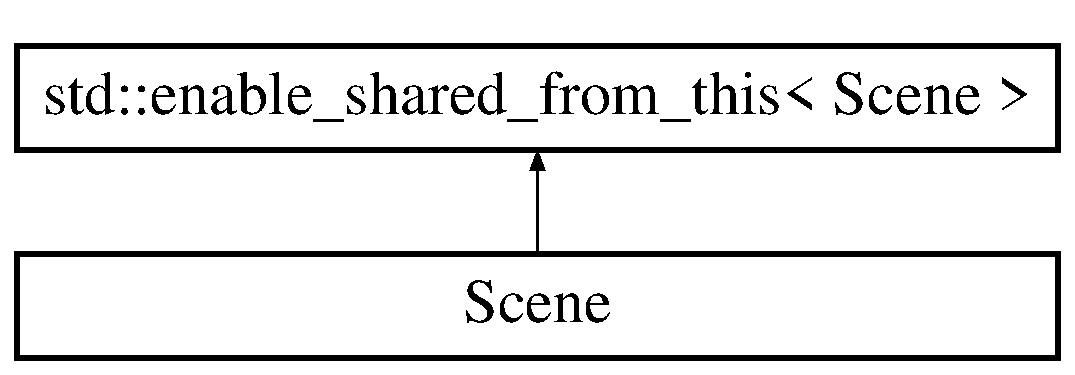
\includegraphics[height=2.000000cm]{class_scene}
\end{center}
\end{figure}
\subsection*{Public Member Functions}
\begin{DoxyCompactItemize}
\item 
\hypertarget{class_scene_a23da430906feb967d70195ef26ba7a88}{}size\+\_\+t {\bfseries Get\+Total\+Objects} () const \label{class_scene_a23da430906feb967d70195ef26ba7a88}

\item 
\hypertarget{class_scene_ab9d522852e85884def3d10600106d724}{}size\+\_\+t {\bfseries Get\+Total\+Lights} () const \label{class_scene_ab9d522852e85884def3d10600106d724}

\item 
\hypertarget{class_scene_acfd7dbaefb2feb8233d2a07d497542d7}{}{\footnotesize template$<$typename T , typename std\+::enable\+\_\+if$<$ std\+::is\+\_\+integral$<$ T $>$\+::value $>$\+::type $\ast$  = nullptr$>$ }\\const \hyperlink{class_scene_object}{Scene\+Object} \& {\bfseries Get\+Scene\+Object} (T index) const \label{class_scene_acfd7dbaefb2feb8233d2a07d497542d7}

\item 
\hypertarget{class_scene_abb610e4c698b3c2ebfb922b5352eba36}{}{\footnotesize template$<$typename T , typename std\+::enable\+\_\+if$<$ std\+::is\+\_\+integral$<$ T $>$\+::value $>$\+::type $\ast$  = nullptr$>$ }\\const \hyperlink{class_light}{Light} $\ast$ {\bfseries Get\+Light\+Object} (T index) const \label{class_scene_abb610e4c698b3c2ebfb922b5352eba36}

\item 
\hypertarget{class_scene_a6e51f14c74c252d231b73d7109b8117e}{}void {\bfseries Add\+Scene\+Object} (std\+::shared\+\_\+ptr$<$ \hyperlink{class_scene_object}{Scene\+Object} $>$ object)\label{class_scene_a6e51f14c74c252d231b73d7109b8117e}

\item 
\hypertarget{class_scene_ab9b1a906b16bf867600fc3f5b734c1d4}{}void {\bfseries Add\+Light} (std\+::shared\+\_\+ptr$<$ \hyperlink{class_light}{Light} $>$ light)\label{class_scene_ab9b1a906b16bf867600fc3f5b734c1d4}

\item 
\hypertarget{class_scene_ac3b0f6126be07f78a61abfac3487e4df}{}void {\bfseries Clear\+Scene} ()\label{class_scene_ac3b0f6126be07f78a61abfac3487e4df}

\end{DoxyCompactItemize}
\subsection*{Friends}
\begin{DoxyCompactItemize}
\item 
\hypertarget{class_scene_a70538530bc36e033e360880ef311df61}{}class {\bfseries Renderer}\label{class_scene_a70538530bc36e033e360880ef311df61}

\end{DoxyCompactItemize}


\subsection{Detailed Description}


Definition at line 11 of file Scene.\+h.



The documentation for this class was generated from the following files\+:\begin{DoxyCompactItemize}
\item 
/\+Users/michaelbao/workspace/cs148opengl4/source/common/\+Scene/Scene.\+h\item 
/\+Users/michaelbao/workspace/cs148opengl4/source/common/\+Scene/Scene.\+cpp\end{DoxyCompactItemize}

\hypertarget{class_scene_object}{}\section{Scene\+Object Class Reference}
\label{class_scene_object}\index{Scene\+Object@{Scene\+Object}}


{\ttfamily \#include $<$Scene\+Object.\+h$>$}

Inheritance diagram for Scene\+Object\+:\begin{figure}[H]
\begin{center}
\leavevmode
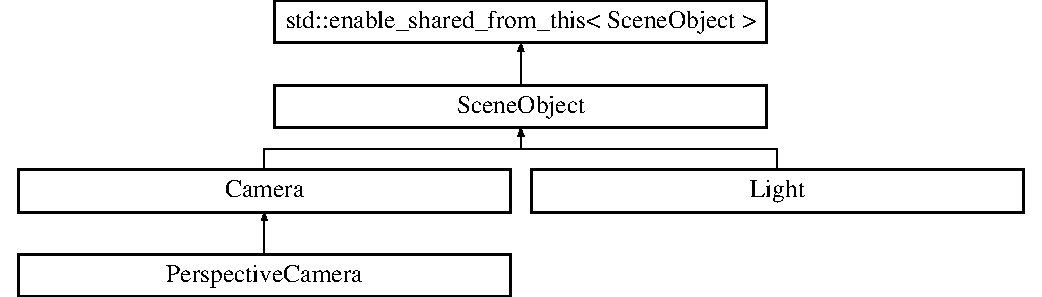
\includegraphics[height=3.985765cm]{class_scene_object}
\end{center}
\end{figure}
\subsection*{Public Member Functions}
\begin{DoxyCompactItemize}
\item 
\hyperlink{class_scene_object_a0d268d96d77dbeb45b07a6442e2f4d0d}{Scene\+Object} ()
\item 
\hyperlink{class_scene_object_a9dd76f946c8e0743bed57f9499773fbd}{Scene\+Object} (std\+::shared\+\_\+ptr$<$ class \hyperlink{class_rendering_object}{Rendering\+Object} $>$ base\+Object)
\item 
\hyperlink{class_scene_object_aa89b21b4732296d196a76d1785aee02c}{Scene\+Object} (const std\+::vector$<$ std\+::shared\+\_\+ptr$<$ class \hyperlink{class_rendering_object}{Rendering\+Object} $>$$>$ \&base\+Objects)
\item 
virtual \hyperlink{class_scene_object_ab258d6b94e982d5ae71ad4d7652381f4}{$\sim$\+Scene\+Object} ()
\item 
virtual void \hyperlink{class_scene_object_a5ab56b2b2997f96aed97415185beec41}{Prepare\+Shader\+For\+Rendering} (const class \hyperlink{class_shader_program}{Shader\+Program} $\ast$shader, const class \hyperlink{class_camera}{Camera} $\ast$current\+Camera, const class \hyperlink{class_light}{Light} $\ast$current\+Light) const 
\item 
size\+\_\+t \hyperlink{class_scene_object_ac2873f8a613bd4b161a1ea605888d6e7}{Get\+Total\+Render\+Objects} () const 
\item 
virtual const class \hyperlink{class_rendering_object}{Rendering\+Object} $\ast$ \hyperlink{class_scene_object_a29b15adf1faeceef0b3f5b1c36e34d5c}{Get\+Render\+Object} (int index=0) const 
\item 
virtual glm\+::mat4 \hyperlink{class_scene_object_aea26bf44c609cc4d733a811a55e442e2}{Get\+Transformation\+Matrix} () const 
\item 
virtual glm\+::vec4 \hyperlink{class_scene_object_abdf46a2b05799382e9cb3894d5da03ea}{Get\+Forward\+Direction} () const 
\item 
virtual glm\+::vec4 \hyperlink{class_scene_object_ab96fed2fb77d81c8d1c2735fbf2a998a}{Get\+Right\+Direction} () const 
\item 
virtual glm\+::vec4 \hyperlink{class_scene_object_ad8828989c033b25c996cf025d7e86f54}{Get\+Up\+Direction} () const 
\item 
void \hyperlink{class_scene_object_a04868377580069b0ee9d202bdb1b7159}{Translate} (const glm\+::vec3 \&translation)
\item 
void \hyperlink{class_scene_object_a0d27f5853e8e1718b1a77f0f1a6d4551}{Rotate} (const glm\+::vec3 \&axis, float radians)
\item 
void \hyperlink{class_scene_object_a00d73ad3f7d77bfc0d3c1869decb97ea}{Mult\+Scale} (float input\+Scale)
\item 
void \hyperlink{class_scene_object_a40d7194cf79cad6ee3a2fa7c3d8ed95c}{Add\+Scale} (float input\+Scale)
\item 
void \hyperlink{class_scene_object_a1903672e77e88a1e220fcfa8e6afc1d4}{Set\+Position} (const glm\+::vec3 \&in)
\item 
glm\+::vec4 \hyperlink{class_scene_object_ac52870b92ce4cebdd153d44754d1ca7c}{Get\+Position} () const 
\end{DoxyCompactItemize}
\subsection*{Static Public Member Functions}
\begin{DoxyCompactItemize}
\item 
static glm\+::vec4 \hyperlink{class_scene_object_a334a5fb4e91d85fe6a046bd83dd235d3}{Get\+World\+Up} ()
\item 
static glm\+::vec4 \hyperlink{class_scene_object_a46d0ffed082f7bd515b9550ef9f9a86a}{Get\+World\+Right} ()
\item 
static glm\+::vec4 \hyperlink{class_scene_object_a6fa71efda895933be4ee684745980e68}{Get\+World\+Forward} ()
\end{DoxyCompactItemize}
\subsection*{Protected Member Functions}
\begin{DoxyCompactItemize}
\item 
virtual void \hyperlink{class_scene_object_a20e31da3f9d2765de50cdb2d637ae6c9}{Update\+Transformation\+Matrix} ()
\end{DoxyCompactItemize}
\subsection*{Protected Attributes}
\begin{DoxyCompactItemize}
\item 
glm\+::mat4 \hyperlink{class_scene_object_aac3f13eea8a7b455e8cffc6eceef211c}{cached\+Transformation\+Matrix}
\item 
glm\+::vec4 \hyperlink{class_scene_object_ab4aa9bed778001970c38ea11ef34b285}{position}
\item 
glm\+::quat \hyperlink{class_scene_object_ae27376aaca87543a75b5a2cd0daf6e2f}{rotation}
\item 
glm\+::vec3 \hyperlink{class_scene_object_a62c686b880fe4f58dec64a409e56de26}{scale}
\end{DoxyCompactItemize}
\subsection*{Static Protected Attributes}
\begin{DoxyCompactItemize}
\item 
static const std\+::string \hyperlink{class_scene_object_a62d236f4f5c52b66bd02d13d09b6ce5e}{M\+O\+D\+E\+L\+\_\+\+M\+A\+T\+R\+I\+X\+\_\+\+L\+O\+C\+A\+T\+I\+O\+N} = \char`\"{}model\+Matrix\char`\"{}
\item 
static const std\+::string \hyperlink{class_scene_object_a1c129ecdd6bd8e2f34c713f5dd183361}{V\+I\+E\+W\+\_\+\+M\+A\+T\+R\+I\+X\+\_\+\+L\+O\+C\+A\+T\+I\+O\+N} = \char`\"{}view\+Matrix\char`\"{}
\item 
static const std\+::string \hyperlink{class_scene_object_ad9a8c9c39a4a262c5e379c0bda184541}{P\+R\+O\+J\+E\+C\+T\+I\+O\+N\+\_\+\+M\+A\+T\+R\+I\+X\+\_\+\+L\+O\+C\+A\+T\+I\+O\+N} = \char`\"{}projection\+Matrix\char`\"{}
\item 
static constexpr float \hyperlink{class_scene_object_a5c61f60925abade4340e7e56c68a989a}{M\+I\+N\+I\+M\+U\+M\+\_\+\+S\+C\+A\+L\+E} = 0.\+01f
\end{DoxyCompactItemize}
\subsection*{Private Attributes}
\begin{DoxyCompactItemize}
\item 
std\+::vector$<$ std\+::shared\+\_\+ptr$<$ class \hyperlink{class_rendering_object}{Rendering\+Object} $>$ $>$ \hyperlink{class_scene_object_a4bbf98a19bd8e7ddd491fbb9a41b42cf}{render\+Object}
\end{DoxyCompactItemize}


\subsection{Detailed Description}


Definition at line 8 of file Scene\+Object.\+h.



\subsection{Constructor \& Destructor Documentation}
\hypertarget{class_scene_object_a0d268d96d77dbeb45b07a6442e2f4d0d}{}\index{Scene\+Object@{Scene\+Object}!Scene\+Object@{Scene\+Object}}
\index{Scene\+Object@{Scene\+Object}!Scene\+Object@{Scene\+Object}}
\subsubsection[{Scene\+Object}]{\setlength{\rightskip}{0pt plus 5cm}Scene\+Object\+::\+Scene\+Object (
\begin{DoxyParamCaption}
{}
\end{DoxyParamCaption}
)}\label{class_scene_object_a0d268d96d77dbeb45b07a6442e2f4d0d}


Definition at line 11 of file Scene\+Object.\+cpp.

\hypertarget{class_scene_object_a9dd76f946c8e0743bed57f9499773fbd}{}\index{Scene\+Object@{Scene\+Object}!Scene\+Object@{Scene\+Object}}
\index{Scene\+Object@{Scene\+Object}!Scene\+Object@{Scene\+Object}}
\subsubsection[{Scene\+Object}]{\setlength{\rightskip}{0pt plus 5cm}Scene\+Object\+::\+Scene\+Object (
\begin{DoxyParamCaption}
\item[{std\+::shared\+\_\+ptr$<$ class {\bf Rendering\+Object} $>$}]{base\+Object}
\end{DoxyParamCaption}
)}\label{class_scene_object_a9dd76f946c8e0743bed57f9499773fbd}


Definition at line 16 of file Scene\+Object.\+cpp.

\hypertarget{class_scene_object_aa89b21b4732296d196a76d1785aee02c}{}\index{Scene\+Object@{Scene\+Object}!Scene\+Object@{Scene\+Object}}
\index{Scene\+Object@{Scene\+Object}!Scene\+Object@{Scene\+Object}}
\subsubsection[{Scene\+Object}]{\setlength{\rightskip}{0pt plus 5cm}Scene\+Object\+::\+Scene\+Object (
\begin{DoxyParamCaption}
\item[{const std\+::vector$<$ std\+::shared\+\_\+ptr$<$ class {\bf Rendering\+Object} $>$$>$ \&}]{base\+Objects}
\end{DoxyParamCaption}
)}\label{class_scene_object_aa89b21b4732296d196a76d1785aee02c}


Definition at line 22 of file Scene\+Object.\+cpp.

\hypertarget{class_scene_object_ab258d6b94e982d5ae71ad4d7652381f4}{}\index{Scene\+Object@{Scene\+Object}!````~Scene\+Object@{$\sim$\+Scene\+Object}}
\index{````~Scene\+Object@{$\sim$\+Scene\+Object}!Scene\+Object@{Scene\+Object}}
\subsubsection[{$\sim$\+Scene\+Object}]{\setlength{\rightskip}{0pt plus 5cm}Scene\+Object\+::$\sim$\+Scene\+Object (
\begin{DoxyParamCaption}
{}
\end{DoxyParamCaption}
)\hspace{0.3cm}{\ttfamily [virtual]}}\label{class_scene_object_ab258d6b94e982d5ae71ad4d7652381f4}


Definition at line 28 of file Scene\+Object.\+cpp.



\subsection{Member Function Documentation}
\hypertarget{class_scene_object_a40d7194cf79cad6ee3a2fa7c3d8ed95c}{}\index{Scene\+Object@{Scene\+Object}!Add\+Scale@{Add\+Scale}}
\index{Add\+Scale@{Add\+Scale}!Scene\+Object@{Scene\+Object}}
\subsubsection[{Add\+Scale}]{\setlength{\rightskip}{0pt plus 5cm}void Scene\+Object\+::\+Add\+Scale (
\begin{DoxyParamCaption}
\item[{float}]{input\+Scale}
\end{DoxyParamCaption}
)}\label{class_scene_object_a40d7194cf79cad6ee3a2fa7c3d8ed95c}


Definition at line 122 of file Scene\+Object.\+cpp.

\hypertarget{class_scene_object_abdf46a2b05799382e9cb3894d5da03ea}{}\index{Scene\+Object@{Scene\+Object}!Get\+Forward\+Direction@{Get\+Forward\+Direction}}
\index{Get\+Forward\+Direction@{Get\+Forward\+Direction}!Scene\+Object@{Scene\+Object}}
\subsubsection[{Get\+Forward\+Direction}]{\setlength{\rightskip}{0pt plus 5cm}glm\+::vec4 Scene\+Object\+::\+Get\+Forward\+Direction (
\begin{DoxyParamCaption}
{}
\end{DoxyParamCaption}
) const\hspace{0.3cm}{\ttfamily [virtual]}}\label{class_scene_object_abdf46a2b05799382e9cb3894d5da03ea}


Definition at line 66 of file Scene\+Object.\+cpp.

\hypertarget{class_scene_object_ac52870b92ce4cebdd153d44754d1ca7c}{}\index{Scene\+Object@{Scene\+Object}!Get\+Position@{Get\+Position}}
\index{Get\+Position@{Get\+Position}!Scene\+Object@{Scene\+Object}}
\subsubsection[{Get\+Position}]{\setlength{\rightskip}{0pt plus 5cm}glm\+::vec4 Scene\+Object\+::\+Get\+Position (
\begin{DoxyParamCaption}
{}
\end{DoxyParamCaption}
) const\hspace{0.3cm}{\ttfamily [inline]}}\label{class_scene_object_ac52870b92ce4cebdd153d44754d1ca7c}


Definition at line 44 of file Scene\+Object.\+h.

\hypertarget{class_scene_object_a29b15adf1faeceef0b3f5b1c36e34d5c}{}\index{Scene\+Object@{Scene\+Object}!Get\+Render\+Object@{Get\+Render\+Object}}
\index{Get\+Render\+Object@{Get\+Render\+Object}!Scene\+Object@{Scene\+Object}}
\subsubsection[{Get\+Render\+Object}]{\setlength{\rightskip}{0pt plus 5cm}const {\bf Rendering\+Object} $\ast$ Scene\+Object\+::\+Get\+Render\+Object (
\begin{DoxyParamCaption}
\item[{int}]{index = {\ttfamily 0}}
\end{DoxyParamCaption}
) const\hspace{0.3cm}{\ttfamily [virtual]}}\label{class_scene_object_a29b15adf1faeceef0b3f5b1c36e34d5c}


Definition at line 46 of file Scene\+Object.\+cpp.

\hypertarget{class_scene_object_ab96fed2fb77d81c8d1c2735fbf2a998a}{}\index{Scene\+Object@{Scene\+Object}!Get\+Right\+Direction@{Get\+Right\+Direction}}
\index{Get\+Right\+Direction@{Get\+Right\+Direction}!Scene\+Object@{Scene\+Object}}
\subsubsection[{Get\+Right\+Direction}]{\setlength{\rightskip}{0pt plus 5cm}glm\+::vec4 Scene\+Object\+::\+Get\+Right\+Direction (
\begin{DoxyParamCaption}
{}
\end{DoxyParamCaption}
) const\hspace{0.3cm}{\ttfamily [virtual]}}\label{class_scene_object_ab96fed2fb77d81c8d1c2735fbf2a998a}


Definition at line 71 of file Scene\+Object.\+cpp.

\hypertarget{class_scene_object_ac2873f8a613bd4b161a1ea605888d6e7}{}\index{Scene\+Object@{Scene\+Object}!Get\+Total\+Render\+Objects@{Get\+Total\+Render\+Objects}}
\index{Get\+Total\+Render\+Objects@{Get\+Total\+Render\+Objects}!Scene\+Object@{Scene\+Object}}
\subsubsection[{Get\+Total\+Render\+Objects}]{\setlength{\rightskip}{0pt plus 5cm}size\+\_\+t Scene\+Object\+::\+Get\+Total\+Render\+Objects (
\begin{DoxyParamCaption}
{}
\end{DoxyParamCaption}
) const\hspace{0.3cm}{\ttfamily [inline]}}\label{class_scene_object_ac2873f8a613bd4b161a1ea605888d6e7}


Definition at line 18 of file Scene\+Object.\+h.

\hypertarget{class_scene_object_aea26bf44c609cc4d733a811a55e442e2}{}\index{Scene\+Object@{Scene\+Object}!Get\+Transformation\+Matrix@{Get\+Transformation\+Matrix}}
\index{Get\+Transformation\+Matrix@{Get\+Transformation\+Matrix}!Scene\+Object@{Scene\+Object}}
\subsubsection[{Get\+Transformation\+Matrix}]{\setlength{\rightskip}{0pt plus 5cm}glm\+::mat4 Scene\+Object\+::\+Get\+Transformation\+Matrix (
\begin{DoxyParamCaption}
{}
\end{DoxyParamCaption}
) const\hspace{0.3cm}{\ttfamily [virtual]}}\label{class_scene_object_aea26bf44c609cc4d733a811a55e442e2}


Definition at line 52 of file Scene\+Object.\+cpp.

\hypertarget{class_scene_object_ad8828989c033b25c996cf025d7e86f54}{}\index{Scene\+Object@{Scene\+Object}!Get\+Up\+Direction@{Get\+Up\+Direction}}
\index{Get\+Up\+Direction@{Get\+Up\+Direction}!Scene\+Object@{Scene\+Object}}
\subsubsection[{Get\+Up\+Direction}]{\setlength{\rightskip}{0pt plus 5cm}glm\+::vec4 Scene\+Object\+::\+Get\+Up\+Direction (
\begin{DoxyParamCaption}
{}
\end{DoxyParamCaption}
) const\hspace{0.3cm}{\ttfamily [virtual]}}\label{class_scene_object_ad8828989c033b25c996cf025d7e86f54}


Definition at line 76 of file Scene\+Object.\+cpp.

\hypertarget{class_scene_object_a6fa71efda895933be4ee684745980e68}{}\index{Scene\+Object@{Scene\+Object}!Get\+World\+Forward@{Get\+World\+Forward}}
\index{Get\+World\+Forward@{Get\+World\+Forward}!Scene\+Object@{Scene\+Object}}
\subsubsection[{Get\+World\+Forward}]{\setlength{\rightskip}{0pt plus 5cm}glm\+::vec4 Scene\+Object\+::\+Get\+World\+Forward (
\begin{DoxyParamCaption}
{}
\end{DoxyParamCaption}
)\hspace{0.3cm}{\ttfamily [static]}}\label{class_scene_object_a6fa71efda895933be4ee684745980e68}


Definition at line 91 of file Scene\+Object.\+cpp.

\hypertarget{class_scene_object_a46d0ffed082f7bd515b9550ef9f9a86a}{}\index{Scene\+Object@{Scene\+Object}!Get\+World\+Right@{Get\+World\+Right}}
\index{Get\+World\+Right@{Get\+World\+Right}!Scene\+Object@{Scene\+Object}}
\subsubsection[{Get\+World\+Right}]{\setlength{\rightskip}{0pt plus 5cm}glm\+::vec4 Scene\+Object\+::\+Get\+World\+Right (
\begin{DoxyParamCaption}
{}
\end{DoxyParamCaption}
)\hspace{0.3cm}{\ttfamily [static]}}\label{class_scene_object_a46d0ffed082f7bd515b9550ef9f9a86a}


Definition at line 86 of file Scene\+Object.\+cpp.

\hypertarget{class_scene_object_a334a5fb4e91d85fe6a046bd83dd235d3}{}\index{Scene\+Object@{Scene\+Object}!Get\+World\+Up@{Get\+World\+Up}}
\index{Get\+World\+Up@{Get\+World\+Up}!Scene\+Object@{Scene\+Object}}
\subsubsection[{Get\+World\+Up}]{\setlength{\rightskip}{0pt plus 5cm}glm\+::vec4 Scene\+Object\+::\+Get\+World\+Up (
\begin{DoxyParamCaption}
{}
\end{DoxyParamCaption}
)\hspace{0.3cm}{\ttfamily [static]}}\label{class_scene_object_a334a5fb4e91d85fe6a046bd83dd235d3}


Definition at line 81 of file Scene\+Object.\+cpp.

\hypertarget{class_scene_object_a00d73ad3f7d77bfc0d3c1869decb97ea}{}\index{Scene\+Object@{Scene\+Object}!Mult\+Scale@{Mult\+Scale}}
\index{Mult\+Scale@{Mult\+Scale}!Scene\+Object@{Scene\+Object}}
\subsubsection[{Mult\+Scale}]{\setlength{\rightskip}{0pt plus 5cm}void Scene\+Object\+::\+Mult\+Scale (
\begin{DoxyParamCaption}
\item[{float}]{input\+Scale}
\end{DoxyParamCaption}
)}\label{class_scene_object_a00d73ad3f7d77bfc0d3c1869decb97ea}


Definition at line 115 of file Scene\+Object.\+cpp.

\hypertarget{class_scene_object_a5ab56b2b2997f96aed97415185beec41}{}\index{Scene\+Object@{Scene\+Object}!Prepare\+Shader\+For\+Rendering@{Prepare\+Shader\+For\+Rendering}}
\index{Prepare\+Shader\+For\+Rendering@{Prepare\+Shader\+For\+Rendering}!Scene\+Object@{Scene\+Object}}
\subsubsection[{Prepare\+Shader\+For\+Rendering}]{\setlength{\rightskip}{0pt plus 5cm}void Scene\+Object\+::\+Prepare\+Shader\+For\+Rendering (
\begin{DoxyParamCaption}
\item[{const class {\bf Shader\+Program} $\ast$}]{shader, }
\item[{const class {\bf Camera} $\ast$}]{current\+Camera, }
\item[{const class {\bf Light} $\ast$}]{current\+Light}
\end{DoxyParamCaption}
) const\hspace{0.3cm}{\ttfamily [virtual]}}\label{class_scene_object_a5ab56b2b2997f96aed97415185beec41}


Definition at line 32 of file Scene\+Object.\+cpp.

\hypertarget{class_scene_object_a0d27f5853e8e1718b1a77f0f1a6d4551}{}\index{Scene\+Object@{Scene\+Object}!Rotate@{Rotate}}
\index{Rotate@{Rotate}!Scene\+Object@{Scene\+Object}}
\subsubsection[{Rotate}]{\setlength{\rightskip}{0pt plus 5cm}void Scene\+Object\+::\+Rotate (
\begin{DoxyParamCaption}
\item[{const glm\+::vec3 \&}]{axis, }
\item[{float}]{radians}
\end{DoxyParamCaption}
)}\label{class_scene_object_a0d27f5853e8e1718b1a77f0f1a6d4551}


Definition at line 108 of file Scene\+Object.\+cpp.

\hypertarget{class_scene_object_a1903672e77e88a1e220fcfa8e6afc1d4}{}\index{Scene\+Object@{Scene\+Object}!Set\+Position@{Set\+Position}}
\index{Set\+Position@{Set\+Position}!Scene\+Object@{Scene\+Object}}
\subsubsection[{Set\+Position}]{\setlength{\rightskip}{0pt plus 5cm}void Scene\+Object\+::\+Set\+Position (
\begin{DoxyParamCaption}
\item[{const glm\+::vec3 \&}]{in}
\end{DoxyParamCaption}
)}\label{class_scene_object_a1903672e77e88a1e220fcfa8e6afc1d4}


Definition at line 96 of file Scene\+Object.\+cpp.

\hypertarget{class_scene_object_a04868377580069b0ee9d202bdb1b7159}{}\index{Scene\+Object@{Scene\+Object}!Translate@{Translate}}
\index{Translate@{Translate}!Scene\+Object@{Scene\+Object}}
\subsubsection[{Translate}]{\setlength{\rightskip}{0pt plus 5cm}void Scene\+Object\+::\+Translate (
\begin{DoxyParamCaption}
\item[{const glm\+::vec3 \&}]{translation}
\end{DoxyParamCaption}
)}\label{class_scene_object_a04868377580069b0ee9d202bdb1b7159}


Definition at line 102 of file Scene\+Object.\+cpp.

\hypertarget{class_scene_object_a20e31da3f9d2765de50cdb2d637ae6c9}{}\index{Scene\+Object@{Scene\+Object}!Update\+Transformation\+Matrix@{Update\+Transformation\+Matrix}}
\index{Update\+Transformation\+Matrix@{Update\+Transformation\+Matrix}!Scene\+Object@{Scene\+Object}}
\subsubsection[{Update\+Transformation\+Matrix}]{\setlength{\rightskip}{0pt plus 5cm}void Scene\+Object\+::\+Update\+Transformation\+Matrix (
\begin{DoxyParamCaption}
{}
\end{DoxyParamCaption}
)\hspace{0.3cm}{\ttfamily [protected]}, {\ttfamily [virtual]}}\label{class_scene_object_a20e31da3f9d2765de50cdb2d637ae6c9}


Reimplemented in \hyperlink{class_perspective_camera_a2f17fb07425e2146d5692805753fa368}{Perspective\+Camera}, and \hyperlink{class_camera_aea640c892a3807671d8ca49616d96eda}{Camera}.



Definition at line 57 of file Scene\+Object.\+cpp.



\subsection{Member Data Documentation}
\hypertarget{class_scene_object_aac3f13eea8a7b455e8cffc6eceef211c}{}\index{Scene\+Object@{Scene\+Object}!cached\+Transformation\+Matrix@{cached\+Transformation\+Matrix}}
\index{cached\+Transformation\+Matrix@{cached\+Transformation\+Matrix}!Scene\+Object@{Scene\+Object}}
\subsubsection[{cached\+Transformation\+Matrix}]{\setlength{\rightskip}{0pt plus 5cm}glm\+::mat4 Scene\+Object\+::cached\+Transformation\+Matrix\hspace{0.3cm}{\ttfamily [protected]}}\label{class_scene_object_aac3f13eea8a7b455e8cffc6eceef211c}


Definition at line 47 of file Scene\+Object.\+h.

\hypertarget{class_scene_object_a5c61f60925abade4340e7e56c68a989a}{}\index{Scene\+Object@{Scene\+Object}!M\+I\+N\+I\+M\+U\+M\+\_\+\+S\+C\+A\+L\+E@{M\+I\+N\+I\+M\+U\+M\+\_\+\+S\+C\+A\+L\+E}}
\index{M\+I\+N\+I\+M\+U\+M\+\_\+\+S\+C\+A\+L\+E@{M\+I\+N\+I\+M\+U\+M\+\_\+\+S\+C\+A\+L\+E}!Scene\+Object@{Scene\+Object}}
\subsubsection[{M\+I\+N\+I\+M\+U\+M\+\_\+\+S\+C\+A\+L\+E}]{\setlength{\rightskip}{0pt plus 5cm}constexpr float Scene\+Object\+::\+M\+I\+N\+I\+M\+U\+M\+\_\+\+S\+C\+A\+L\+E = 0.\+01f\hspace{0.3cm}{\ttfamily [static]}, {\ttfamily [protected]}}\label{class_scene_object_a5c61f60925abade4340e7e56c68a989a}


Definition at line 56 of file Scene\+Object.\+h.

\hypertarget{class_scene_object_a62d236f4f5c52b66bd02d13d09b6ce5e}{}\index{Scene\+Object@{Scene\+Object}!M\+O\+D\+E\+L\+\_\+\+M\+A\+T\+R\+I\+X\+\_\+\+L\+O\+C\+A\+T\+I\+O\+N@{M\+O\+D\+E\+L\+\_\+\+M\+A\+T\+R\+I\+X\+\_\+\+L\+O\+C\+A\+T\+I\+O\+N}}
\index{M\+O\+D\+E\+L\+\_\+\+M\+A\+T\+R\+I\+X\+\_\+\+L\+O\+C\+A\+T\+I\+O\+N@{M\+O\+D\+E\+L\+\_\+\+M\+A\+T\+R\+I\+X\+\_\+\+L\+O\+C\+A\+T\+I\+O\+N}!Scene\+Object@{Scene\+Object}}
\subsubsection[{M\+O\+D\+E\+L\+\_\+\+M\+A\+T\+R\+I\+X\+\_\+\+L\+O\+C\+A\+T\+I\+O\+N}]{\setlength{\rightskip}{0pt plus 5cm}const std\+::string Scene\+Object\+::\+M\+O\+D\+E\+L\+\_\+\+M\+A\+T\+R\+I\+X\+\_\+\+L\+O\+C\+A\+T\+I\+O\+N = \char`\"{}model\+Matrix\char`\"{}\hspace{0.3cm}{\ttfamily [static]}, {\ttfamily [protected]}}\label{class_scene_object_a62d236f4f5c52b66bd02d13d09b6ce5e}


Definition at line 53 of file Scene\+Object.\+h.

\hypertarget{class_scene_object_ab4aa9bed778001970c38ea11ef34b285}{}\index{Scene\+Object@{Scene\+Object}!position@{position}}
\index{position@{position}!Scene\+Object@{Scene\+Object}}
\subsubsection[{position}]{\setlength{\rightskip}{0pt plus 5cm}glm\+::vec4 Scene\+Object\+::position\hspace{0.3cm}{\ttfamily [protected]}}\label{class_scene_object_ab4aa9bed778001970c38ea11ef34b285}


Definition at line 49 of file Scene\+Object.\+h.

\hypertarget{class_scene_object_ad9a8c9c39a4a262c5e379c0bda184541}{}\index{Scene\+Object@{Scene\+Object}!P\+R\+O\+J\+E\+C\+T\+I\+O\+N\+\_\+\+M\+A\+T\+R\+I\+X\+\_\+\+L\+O\+C\+A\+T\+I\+O\+N@{P\+R\+O\+J\+E\+C\+T\+I\+O\+N\+\_\+\+M\+A\+T\+R\+I\+X\+\_\+\+L\+O\+C\+A\+T\+I\+O\+N}}
\index{P\+R\+O\+J\+E\+C\+T\+I\+O\+N\+\_\+\+M\+A\+T\+R\+I\+X\+\_\+\+L\+O\+C\+A\+T\+I\+O\+N@{P\+R\+O\+J\+E\+C\+T\+I\+O\+N\+\_\+\+M\+A\+T\+R\+I\+X\+\_\+\+L\+O\+C\+A\+T\+I\+O\+N}!Scene\+Object@{Scene\+Object}}
\subsubsection[{P\+R\+O\+J\+E\+C\+T\+I\+O\+N\+\_\+\+M\+A\+T\+R\+I\+X\+\_\+\+L\+O\+C\+A\+T\+I\+O\+N}]{\setlength{\rightskip}{0pt plus 5cm}const std\+::string Scene\+Object\+::\+P\+R\+O\+J\+E\+C\+T\+I\+O\+N\+\_\+\+M\+A\+T\+R\+I\+X\+\_\+\+L\+O\+C\+A\+T\+I\+O\+N = \char`\"{}projection\+Matrix\char`\"{}\hspace{0.3cm}{\ttfamily [static]}, {\ttfamily [protected]}}\label{class_scene_object_ad9a8c9c39a4a262c5e379c0bda184541}


Definition at line 55 of file Scene\+Object.\+h.

\hypertarget{class_scene_object_a4bbf98a19bd8e7ddd491fbb9a41b42cf}{}\index{Scene\+Object@{Scene\+Object}!render\+Object@{render\+Object}}
\index{render\+Object@{render\+Object}!Scene\+Object@{Scene\+Object}}
\subsubsection[{render\+Object}]{\setlength{\rightskip}{0pt plus 5cm}std\+::vector$<$std\+::shared\+\_\+ptr$<$class {\bf Rendering\+Object}$>$ $>$ Scene\+Object\+::render\+Object\hspace{0.3cm}{\ttfamily [private]}}\label{class_scene_object_a4bbf98a19bd8e7ddd491fbb9a41b42cf}


Definition at line 59 of file Scene\+Object.\+h.

\hypertarget{class_scene_object_ae27376aaca87543a75b5a2cd0daf6e2f}{}\index{Scene\+Object@{Scene\+Object}!rotation@{rotation}}
\index{rotation@{rotation}!Scene\+Object@{Scene\+Object}}
\subsubsection[{rotation}]{\setlength{\rightskip}{0pt plus 5cm}glm\+::quat Scene\+Object\+::rotation\hspace{0.3cm}{\ttfamily [protected]}}\label{class_scene_object_ae27376aaca87543a75b5a2cd0daf6e2f}


Definition at line 50 of file Scene\+Object.\+h.

\hypertarget{class_scene_object_a62c686b880fe4f58dec64a409e56de26}{}\index{Scene\+Object@{Scene\+Object}!scale@{scale}}
\index{scale@{scale}!Scene\+Object@{Scene\+Object}}
\subsubsection[{scale}]{\setlength{\rightskip}{0pt plus 5cm}glm\+::vec3 Scene\+Object\+::scale\hspace{0.3cm}{\ttfamily [protected]}}\label{class_scene_object_a62c686b880fe4f58dec64a409e56de26}


Definition at line 51 of file Scene\+Object.\+h.

\hypertarget{class_scene_object_a1c129ecdd6bd8e2f34c713f5dd183361}{}\index{Scene\+Object@{Scene\+Object}!V\+I\+E\+W\+\_\+\+M\+A\+T\+R\+I\+X\+\_\+\+L\+O\+C\+A\+T\+I\+O\+N@{V\+I\+E\+W\+\_\+\+M\+A\+T\+R\+I\+X\+\_\+\+L\+O\+C\+A\+T\+I\+O\+N}}
\index{V\+I\+E\+W\+\_\+\+M\+A\+T\+R\+I\+X\+\_\+\+L\+O\+C\+A\+T\+I\+O\+N@{V\+I\+E\+W\+\_\+\+M\+A\+T\+R\+I\+X\+\_\+\+L\+O\+C\+A\+T\+I\+O\+N}!Scene\+Object@{Scene\+Object}}
\subsubsection[{V\+I\+E\+W\+\_\+\+M\+A\+T\+R\+I\+X\+\_\+\+L\+O\+C\+A\+T\+I\+O\+N}]{\setlength{\rightskip}{0pt plus 5cm}const std\+::string Scene\+Object\+::\+V\+I\+E\+W\+\_\+\+M\+A\+T\+R\+I\+X\+\_\+\+L\+O\+C\+A\+T\+I\+O\+N = \char`\"{}view\+Matrix\char`\"{}\hspace{0.3cm}{\ttfamily [static]}, {\ttfamily [protected]}}\label{class_scene_object_a1c129ecdd6bd8e2f34c713f5dd183361}


Definition at line 54 of file Scene\+Object.\+h.



The documentation for this class was generated from the following files\+:\begin{DoxyCompactItemize}
\item 
/\+Users/michaelbao/workspace/cs148opengl4/source/common/\+Scene/\hyperlink{_scene_object_8h}{Scene\+Object.\+h}\item 
/\+Users/michaelbao/workspace/cs148opengl4/source/common/\+Scene/\hyperlink{_scene_object_8cpp}{Scene\+Object.\+cpp}\end{DoxyCompactItemize}

\hypertarget{class_shader_program}{}\section{Shader\+Program Class Reference}
\label{class_shader_program}\index{Shader\+Program@{Shader\+Program}}


{\ttfamily \#include $<$Shader\+Program.\+h$>$}

Inheritance diagram for Shader\+Program\+:\begin{figure}[H]
\begin{center}
\leavevmode
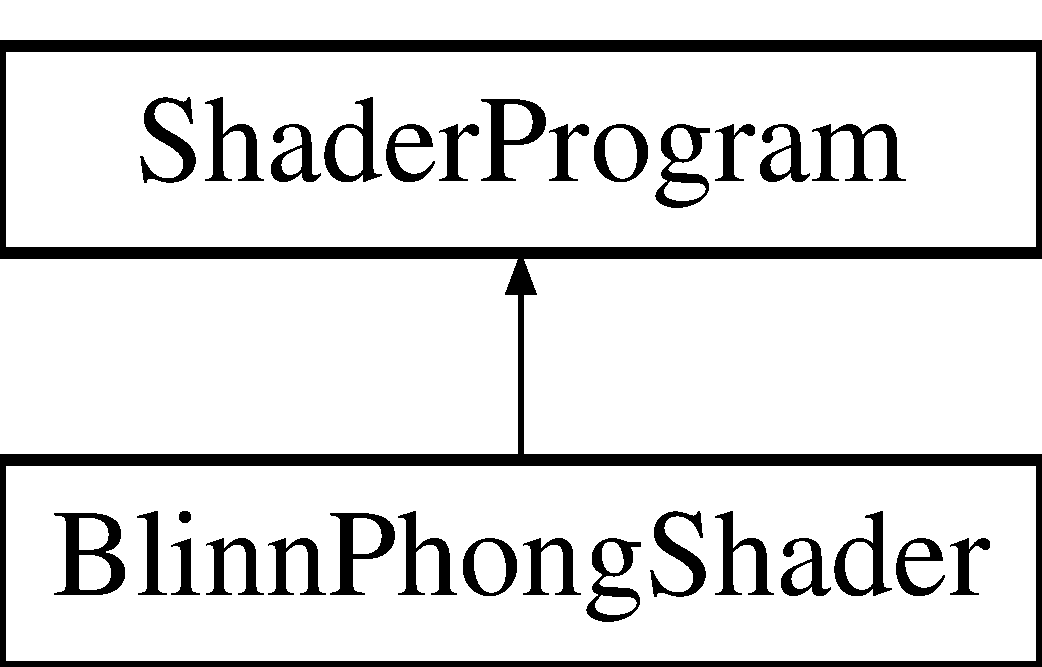
\includegraphics[height=2.000000cm]{class_shader_program}
\end{center}
\end{figure}
\subsection*{Public Member Functions}
\begin{DoxyCompactItemize}
\item 
\hyperlink{class_shader_program_aba2db5734b2f70cc34078126ad279588}{Shader\+Program} (const std\+::unordered\+\_\+map$<$ G\+Lenum, std\+::string $>$ \&input\+Shaders)
\item 
virtual \hyperlink{class_shader_program_a2d2eadcfc48cc2e2ddb82aba70553a9f}{$\sim$\+Shader\+Program} ()
\item 
virtual void \hyperlink{class_shader_program_a906b0232f27663b28cc800ac2851541f}{Start\+Use\+Shader} () const 
\item 
virtual void \hyperlink{class_shader_program_a5afb6f91d30b6e197fab0827c416c51f}{Stop\+Use\+Shader} () const 
\item 
G\+Luint \hyperlink{class_shader_program_a281396edbb786eacf86ae4997a3e90c6}{Get\+Program} () const 
\item 
virtual void \hyperlink{class_shader_program_a2f3c1c149aa0988e07e0a513c69c1770}{Setup\+Shader\+Lighting} (const class \hyperlink{class_light}{Light} $\ast$light) const 
\item 
virtual void \hyperlink{class_shader_program_ad7a595a10717c6051d6c582c850c4ed7}{Setup\+Shader\+Materials} () const 
\item 
virtual void \hyperlink{class_shader_program_a75e888f885b9028847e2d9556a754170}{Setup\+Shader\+Camera} (const class \hyperlink{class_camera}{Camera} $\ast$camera) const 
\item 
void \hyperlink{class_shader_program_a47298abb4ffc8d75f88b3d603aa989f9}{Set\+Shader\+Uniform} (const std\+::string \&location, const glm\+::mat4 \&value) const 
\item 
void \hyperlink{class_shader_program_a3a4c9cd6967787bded962acd7ce6b3c6}{Set\+Shader\+Uniform} (const std\+::string \&location, float value) const 
\item 
void \hyperlink{class_shader_program_a93e7090cc8ff284bfcde6ae972aa5b9e}{Set\+Shader\+Uniform} (const std\+::string \&location, int value) const 
\item 
void \hyperlink{class_shader_program_a08b8936758c067aad38e6cd94608663f}{Set\+Shader\+Uniform} (const std\+::string \&location, const glm\+::vec4 \&value) const 
\item 
void \hyperlink{class_shader_program_ae2e00fa2f9107b34c758996021574b15}{Set\+Shader\+Subroutine} (const std\+::string \&location, const std\+::string \&subroutine, G\+Lenum substage) const 
\item 
{\footnotesize template$<$int N$>$ }\\void \hyperlink{class_shader_program_a16169356d5ce43e64e6018ad5d79f594}{Setup\+Uniform\+Block} (const std\+::string \&block\+Name, const std\+::array$<$ const char $\ast$, N $>$ \&names, std\+::array$<$ G\+Luint, N $>$ \&indices, std\+::array$<$ G\+Lint, N $>$ \&offsets, std\+::vector$<$ G\+Lubyte $>$ \&data, G\+Luint \&block\+Location, G\+Lint \&block\+Size, G\+Luint \&buffer\+Location)
\end{DoxyCompactItemize}
\subsection*{Static Public Member Functions}
\begin{DoxyCompactItemize}
\item 
static std\+::unique\+\_\+ptr$<$ struct \hyperlink{struct_light_properties}{Light\+Properties} $>$ \hyperlink{class_shader_program_a9c09a5050b37c958e07ce4d9756421b9}{Create\+Light\+Properties} ()
\end{DoxyCompactItemize}
\subsection*{Static Protected Member Functions}
\begin{DoxyCompactItemize}
\item 
static G\+Luint \hyperlink{class_shader_program_ab5c50c33203cf65b7f6ffe00d2243d5a}{Load\+Shader\+Object} (G\+Lenum type, const std\+::string \&filename)
\end{DoxyCompactItemize}
\subsection*{Protected Attributes}
\begin{DoxyCompactItemize}
\item 
G\+Luint \hyperlink{class_shader_program_a7d8f2b643a81ac4097606e43ade92f81}{shader\+Program}
\end{DoxyCompactItemize}
\subsection*{Private Attributes}
\begin{DoxyCompactItemize}
\item 
std\+::unordered\+\_\+map$<$ G\+Lenum, G\+Luint $>$ \hyperlink{class_shader_program_a8eabcc4ff693bc9430daef8cfc6008de}{shader\+Objects}
\end{DoxyCompactItemize}
\subsection*{Static Private Attributes}
\begin{DoxyCompactItemize}
\item 
static constexpr int \hyperlink{class_shader_program_a6dfa734f6cd9bdd1debf1a6f39bdfa05}{S\+H\+A\+D\+E\+R\+\_\+\+E\+R\+R\+O\+R\+\_\+\+L\+O\+G\+\_\+\+S\+I\+Z\+E} = 500
\end{DoxyCompactItemize}


\subsection{Detailed Description}


Definition at line 8 of file Shader\+Program.\+h.



\subsection{Constructor \& Destructor Documentation}
\hypertarget{class_shader_program_aba2db5734b2f70cc34078126ad279588}{}\index{Shader\+Program@{Shader\+Program}!Shader\+Program@{Shader\+Program}}
\index{Shader\+Program@{Shader\+Program}!Shader\+Program@{Shader\+Program}}
\subsubsection[{Shader\+Program}]{\setlength{\rightskip}{0pt plus 5cm}Shader\+Program\+::\+Shader\+Program (
\begin{DoxyParamCaption}
\item[{const std\+::unordered\+\_\+map$<$ G\+Lenum, std\+::string $>$ \&}]{input\+Shaders}
\end{DoxyParamCaption}
)}\label{class_shader_program_aba2db5734b2f70cc34078126ad279588}


Definition at line 13 of file Shader\+Program.\+cpp.

\hypertarget{class_shader_program_a2d2eadcfc48cc2e2ddb82aba70553a9f}{}\index{Shader\+Program@{Shader\+Program}!````~Shader\+Program@{$\sim$\+Shader\+Program}}
\index{````~Shader\+Program@{$\sim$\+Shader\+Program}!Shader\+Program@{Shader\+Program}}
\subsubsection[{$\sim$\+Shader\+Program}]{\setlength{\rightskip}{0pt plus 5cm}Shader\+Program\+::$\sim$\+Shader\+Program (
\begin{DoxyParamCaption}
{}
\end{DoxyParamCaption}
)\hspace{0.3cm}{\ttfamily [virtual]}}\label{class_shader_program_a2d2eadcfc48cc2e2ddb82aba70553a9f}


Definition at line 63 of file Shader\+Program.\+cpp.



\subsection{Member Function Documentation}
\hypertarget{class_shader_program_a9c09a5050b37c958e07ce4d9756421b9}{}\index{Shader\+Program@{Shader\+Program}!Create\+Light\+Properties@{Create\+Light\+Properties}}
\index{Create\+Light\+Properties@{Create\+Light\+Properties}!Shader\+Program@{Shader\+Program}}
\subsubsection[{Create\+Light\+Properties}]{\setlength{\rightskip}{0pt plus 5cm}std\+::unique\+\_\+ptr$<$ {\bf Light\+Properties} $>$ Shader\+Program\+::\+Create\+Light\+Properties (
\begin{DoxyParamCaption}
{}
\end{DoxyParamCaption}
)\hspace{0.3cm}{\ttfamily [static]}}\label{class_shader_program_a9c09a5050b37c958e07ce4d9756421b9}


Definition at line 169 of file Shader\+Program.\+cpp.

\hypertarget{class_shader_program_a281396edbb786eacf86ae4997a3e90c6}{}\index{Shader\+Program@{Shader\+Program}!Get\+Program@{Get\+Program}}
\index{Get\+Program@{Get\+Program}!Shader\+Program@{Shader\+Program}}
\subsubsection[{Get\+Program}]{\setlength{\rightskip}{0pt plus 5cm}G\+Luint Shader\+Program\+::\+Get\+Program (
\begin{DoxyParamCaption}
{}
\end{DoxyParamCaption}
) const\hspace{0.3cm}{\ttfamily [inline]}}\label{class_shader_program_a281396edbb786eacf86ae4997a3e90c6}


Definition at line 17 of file Shader\+Program.\+h.

\hypertarget{class_shader_program_ab5c50c33203cf65b7f6ffe00d2243d5a}{}\index{Shader\+Program@{Shader\+Program}!Load\+Shader\+Object@{Load\+Shader\+Object}}
\index{Load\+Shader\+Object@{Load\+Shader\+Object}!Shader\+Program@{Shader\+Program}}
\subsubsection[{Load\+Shader\+Object}]{\setlength{\rightskip}{0pt plus 5cm}G\+Luint Shader\+Program\+::\+Load\+Shader\+Object (
\begin{DoxyParamCaption}
\item[{G\+Lenum}]{type, }
\item[{const std\+::string \&}]{filename}
\end{DoxyParamCaption}
)\hspace{0.3cm}{\ttfamily [static]}, {\ttfamily [protected]}}\label{class_shader_program_ab5c50c33203cf65b7f6ffe00d2243d5a}


Definition at line 68 of file Shader\+Program.\+cpp.

\hypertarget{class_shader_program_ae2e00fa2f9107b34c758996021574b15}{}\index{Shader\+Program@{Shader\+Program}!Set\+Shader\+Subroutine@{Set\+Shader\+Subroutine}}
\index{Set\+Shader\+Subroutine@{Set\+Shader\+Subroutine}!Shader\+Program@{Shader\+Program}}
\subsubsection[{Set\+Shader\+Subroutine}]{\setlength{\rightskip}{0pt plus 5cm}void Shader\+Program\+::\+Set\+Shader\+Subroutine (
\begin{DoxyParamCaption}
\item[{const std\+::string \&}]{location, }
\item[{const std\+::string \&}]{subroutine, }
\item[{G\+Lenum}]{substage}
\end{DoxyParamCaption}
) const}\label{class_shader_program_ae2e00fa2f9107b34c758996021574b15}


Definition at line 138 of file Shader\+Program.\+cpp.

\hypertarget{class_shader_program_a47298abb4ffc8d75f88b3d603aa989f9}{}\index{Shader\+Program@{Shader\+Program}!Set\+Shader\+Uniform@{Set\+Shader\+Uniform}}
\index{Set\+Shader\+Uniform@{Set\+Shader\+Uniform}!Shader\+Program@{Shader\+Program}}
\subsubsection[{Set\+Shader\+Uniform}]{\setlength{\rightskip}{0pt plus 5cm}void Shader\+Program\+::\+Set\+Shader\+Uniform (
\begin{DoxyParamCaption}
\item[{const std\+::string \&}]{location, }
\item[{const glm\+::mat4 \&}]{value}
\end{DoxyParamCaption}
) const}\label{class_shader_program_a47298abb4ffc8d75f88b3d603aa989f9}


Definition at line 113 of file Shader\+Program.\+cpp.

\hypertarget{class_shader_program_a3a4c9cd6967787bded962acd7ce6b3c6}{}\index{Shader\+Program@{Shader\+Program}!Set\+Shader\+Uniform@{Set\+Shader\+Uniform}}
\index{Set\+Shader\+Uniform@{Set\+Shader\+Uniform}!Shader\+Program@{Shader\+Program}}
\subsubsection[{Set\+Shader\+Uniform}]{\setlength{\rightskip}{0pt plus 5cm}void Shader\+Program\+::\+Set\+Shader\+Uniform (
\begin{DoxyParamCaption}
\item[{const std\+::string \&}]{location, }
\item[{float}]{value}
\end{DoxyParamCaption}
) const}\label{class_shader_program_a3a4c9cd6967787bded962acd7ce6b3c6}


Definition at line 125 of file Shader\+Program.\+cpp.

\hypertarget{class_shader_program_a93e7090cc8ff284bfcde6ae972aa5b9e}{}\index{Shader\+Program@{Shader\+Program}!Set\+Shader\+Uniform@{Set\+Shader\+Uniform}}
\index{Set\+Shader\+Uniform@{Set\+Shader\+Uniform}!Shader\+Program@{Shader\+Program}}
\subsubsection[{Set\+Shader\+Uniform}]{\setlength{\rightskip}{0pt plus 5cm}void Shader\+Program\+::\+Set\+Shader\+Uniform (
\begin{DoxyParamCaption}
\item[{const std\+::string \&}]{location, }
\item[{int}]{value}
\end{DoxyParamCaption}
) const}\label{class_shader_program_a93e7090cc8ff284bfcde6ae972aa5b9e}


Definition at line 119 of file Shader\+Program.\+cpp.

\hypertarget{class_shader_program_a08b8936758c067aad38e6cd94608663f}{}\index{Shader\+Program@{Shader\+Program}!Set\+Shader\+Uniform@{Set\+Shader\+Uniform}}
\index{Set\+Shader\+Uniform@{Set\+Shader\+Uniform}!Shader\+Program@{Shader\+Program}}
\subsubsection[{Set\+Shader\+Uniform}]{\setlength{\rightskip}{0pt plus 5cm}void Shader\+Program\+::\+Set\+Shader\+Uniform (
\begin{DoxyParamCaption}
\item[{const std\+::string \&}]{location, }
\item[{const glm\+::vec4 \&}]{value}
\end{DoxyParamCaption}
) const}\label{class_shader_program_a08b8936758c067aad38e6cd94608663f}


Definition at line 131 of file Shader\+Program.\+cpp.

\hypertarget{class_shader_program_a75e888f885b9028847e2d9556a754170}{}\index{Shader\+Program@{Shader\+Program}!Setup\+Shader\+Camera@{Setup\+Shader\+Camera}}
\index{Setup\+Shader\+Camera@{Setup\+Shader\+Camera}!Shader\+Program@{Shader\+Program}}
\subsubsection[{Setup\+Shader\+Camera}]{\setlength{\rightskip}{0pt plus 5cm}void Shader\+Program\+::\+Setup\+Shader\+Camera (
\begin{DoxyParamCaption}
\item[{const class {\bf Camera} $\ast$}]{camera}
\end{DoxyParamCaption}
) const\hspace{0.3cm}{\ttfamily [virtual]}}\label{class_shader_program_a75e888f885b9028847e2d9556a754170}


Reimplemented in \hyperlink{class_blinn_phong_shader_a0e3e2e1d5981f173a72e82d0ef4d643d}{Blinn\+Phong\+Shader}.



Definition at line 165 of file Shader\+Program.\+cpp.

\hypertarget{class_shader_program_a2f3c1c149aa0988e07e0a513c69c1770}{}\index{Shader\+Program@{Shader\+Program}!Setup\+Shader\+Lighting@{Setup\+Shader\+Lighting}}
\index{Setup\+Shader\+Lighting@{Setup\+Shader\+Lighting}!Shader\+Program@{Shader\+Program}}
\subsubsection[{Setup\+Shader\+Lighting}]{\setlength{\rightskip}{0pt plus 5cm}void Shader\+Program\+::\+Setup\+Shader\+Lighting (
\begin{DoxyParamCaption}
\item[{const class {\bf Light} $\ast$}]{light}
\end{DoxyParamCaption}
) const\hspace{0.3cm}{\ttfamily [virtual]}}\label{class_shader_program_a2f3c1c149aa0988e07e0a513c69c1770}


Reimplemented in \hyperlink{class_blinn_phong_shader_a9e4a7358ce59f7fa77ed872eb15eabe7}{Blinn\+Phong\+Shader}.



Definition at line 157 of file Shader\+Program.\+cpp.

\hypertarget{class_shader_program_ad7a595a10717c6051d6c582c850c4ed7}{}\index{Shader\+Program@{Shader\+Program}!Setup\+Shader\+Materials@{Setup\+Shader\+Materials}}
\index{Setup\+Shader\+Materials@{Setup\+Shader\+Materials}!Shader\+Program@{Shader\+Program}}
\subsubsection[{Setup\+Shader\+Materials}]{\setlength{\rightskip}{0pt plus 5cm}void Shader\+Program\+::\+Setup\+Shader\+Materials (
\begin{DoxyParamCaption}
{}
\end{DoxyParamCaption}
) const\hspace{0.3cm}{\ttfamily [virtual]}}\label{class_shader_program_ad7a595a10717c6051d6c582c850c4ed7}


Reimplemented in \hyperlink{class_blinn_phong_shader_ade1dfa6ceb0b2650b2ca3b849ee875ac}{Blinn\+Phong\+Shader}.



Definition at line 161 of file Shader\+Program.\+cpp.

\hypertarget{class_shader_program_a16169356d5ce43e64e6018ad5d79f594}{}\index{Shader\+Program@{Shader\+Program}!Setup\+Uniform\+Block@{Setup\+Uniform\+Block}}
\index{Setup\+Uniform\+Block@{Setup\+Uniform\+Block}!Shader\+Program@{Shader\+Program}}
\subsubsection[{Setup\+Uniform\+Block}]{\setlength{\rightskip}{0pt plus 5cm}template$<$int N$>$ void Shader\+Program\+::\+Setup\+Uniform\+Block (
\begin{DoxyParamCaption}
\item[{const std\+::string \&}]{block\+Name, }
\item[{const std\+::array$<$ const char $\ast$, N $>$ \&}]{names, }
\item[{std\+::array$<$ G\+Luint, N $>$ \&}]{indices, }
\item[{std\+::array$<$ G\+Lint, N $>$ \&}]{offsets, }
\item[{std\+::vector$<$ G\+Lubyte $>$ \&}]{data, }
\item[{G\+Luint \&}]{block\+Location, }
\item[{G\+Lint \&}]{block\+Size, }
\item[{G\+Luint \&}]{buffer\+Location}
\end{DoxyParamCaption}
)\hspace{0.3cm}{\ttfamily [inline]}}\label{class_shader_program_a16169356d5ce43e64e6018ad5d79f594}


Definition at line 31 of file Shader\+Program.\+h.

\hypertarget{class_shader_program_a906b0232f27663b28cc800ac2851541f}{}\index{Shader\+Program@{Shader\+Program}!Start\+Use\+Shader@{Start\+Use\+Shader}}
\index{Start\+Use\+Shader@{Start\+Use\+Shader}!Shader\+Program@{Shader\+Program}}
\subsubsection[{Start\+Use\+Shader}]{\setlength{\rightskip}{0pt plus 5cm}void Shader\+Program\+::\+Start\+Use\+Shader (
\begin{DoxyParamCaption}
{}
\end{DoxyParamCaption}
) const\hspace{0.3cm}{\ttfamily [virtual]}}\label{class_shader_program_a906b0232f27663b28cc800ac2851541f}


Definition at line 103 of file Shader\+Program.\+cpp.

\hypertarget{class_shader_program_a5afb6f91d30b6e197fab0827c416c51f}{}\index{Shader\+Program@{Shader\+Program}!Stop\+Use\+Shader@{Stop\+Use\+Shader}}
\index{Stop\+Use\+Shader@{Stop\+Use\+Shader}!Shader\+Program@{Shader\+Program}}
\subsubsection[{Stop\+Use\+Shader}]{\setlength{\rightskip}{0pt plus 5cm}void Shader\+Program\+::\+Stop\+Use\+Shader (
\begin{DoxyParamCaption}
{}
\end{DoxyParamCaption}
) const\hspace{0.3cm}{\ttfamily [virtual]}}\label{class_shader_program_a5afb6f91d30b6e197fab0827c416c51f}


Definition at line 108 of file Shader\+Program.\+cpp.



\subsection{Member Data Documentation}
\hypertarget{class_shader_program_a6dfa734f6cd9bdd1debf1a6f39bdfa05}{}\index{Shader\+Program@{Shader\+Program}!S\+H\+A\+D\+E\+R\+\_\+\+E\+R\+R\+O\+R\+\_\+\+L\+O\+G\+\_\+\+S\+I\+Z\+E@{S\+H\+A\+D\+E\+R\+\_\+\+E\+R\+R\+O\+R\+\_\+\+L\+O\+G\+\_\+\+S\+I\+Z\+E}}
\index{S\+H\+A\+D\+E\+R\+\_\+\+E\+R\+R\+O\+R\+\_\+\+L\+O\+G\+\_\+\+S\+I\+Z\+E@{S\+H\+A\+D\+E\+R\+\_\+\+E\+R\+R\+O\+R\+\_\+\+L\+O\+G\+\_\+\+S\+I\+Z\+E}!Shader\+Program@{Shader\+Program}}
\subsubsection[{S\+H\+A\+D\+E\+R\+\_\+\+E\+R\+R\+O\+R\+\_\+\+L\+O\+G\+\_\+\+S\+I\+Z\+E}]{\setlength{\rightskip}{0pt plus 5cm}constexpr int Shader\+Program\+::\+S\+H\+A\+D\+E\+R\+\_\+\+E\+R\+R\+O\+R\+\_\+\+L\+O\+G\+\_\+\+S\+I\+Z\+E = 500\hspace{0.3cm}{\ttfamily [static]}, {\ttfamily [private]}}\label{class_shader_program_a6dfa734f6cd9bdd1debf1a6f39bdfa05}


Definition at line 64 of file Shader\+Program.\+h.

\hypertarget{class_shader_program_a8eabcc4ff693bc9430daef8cfc6008de}{}\index{Shader\+Program@{Shader\+Program}!shader\+Objects@{shader\+Objects}}
\index{shader\+Objects@{shader\+Objects}!Shader\+Program@{Shader\+Program}}
\subsubsection[{shader\+Objects}]{\setlength{\rightskip}{0pt plus 5cm}std\+::unordered\+\_\+map$<$G\+Lenum, G\+Luint$>$ Shader\+Program\+::shader\+Objects\hspace{0.3cm}{\ttfamily [private]}}\label{class_shader_program_a8eabcc4ff693bc9430daef8cfc6008de}


Definition at line 62 of file Shader\+Program.\+h.

\hypertarget{class_shader_program_a7d8f2b643a81ac4097606e43ade92f81}{}\index{Shader\+Program@{Shader\+Program}!shader\+Program@{shader\+Program}}
\index{shader\+Program@{shader\+Program}!Shader\+Program@{Shader\+Program}}
\subsubsection[{shader\+Program}]{\setlength{\rightskip}{0pt plus 5cm}G\+Luint Shader\+Program\+::shader\+Program\hspace{0.3cm}{\ttfamily [protected]}}\label{class_shader_program_a7d8f2b643a81ac4097606e43ade92f81}


Definition at line 60 of file Shader\+Program.\+h.



The documentation for this class was generated from the following files\+:\begin{DoxyCompactItemize}
\item 
/\+Users/michaelbao/workspace/cs148opengl4/source/common/\+Rendering/\+Shaders/\hyperlink{_shader_program_8h}{Shader\+Program.\+h}\item 
/\+Users/michaelbao/workspace/cs148opengl4/source/common/\+Rendering/\+Shaders/\hyperlink{_shader_program_8cpp}{Shader\+Program.\+cpp}\end{DoxyCompactItemize}

\hypertarget{class_texture}{}\section{Texture Class Reference}
\label{class_texture}\index{Texture@{Texture}}


{\ttfamily \#include $<$Texture.\+h$>$}

Inheritance diagram for Texture\+:\begin{figure}[H]
\begin{center}
\leavevmode
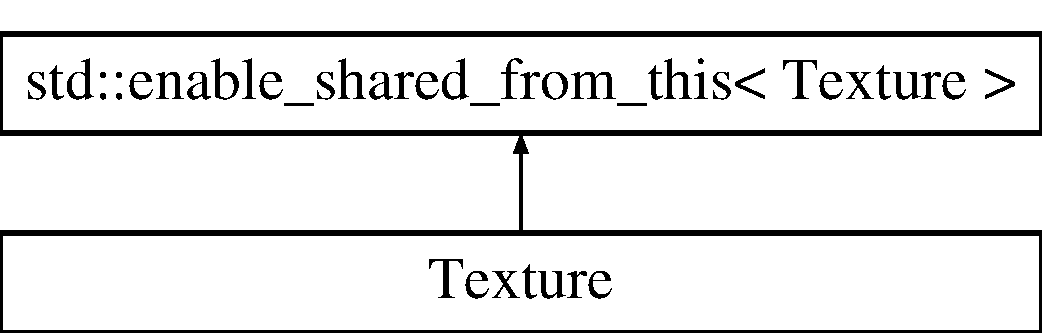
\includegraphics[height=2.000000cm]{class_texture}
\end{center}
\end{figure}
\subsection*{Public Member Functions}
\begin{DoxyCompactItemize}
\item 
\hyperlink{class_texture_ad2772674616f4956ba602d0853ca5585}{Texture} (G\+Lubyte $\ast$raw\+Data, int width, int height)
\item 
virtual \hyperlink{class_texture_a09c4bcb7462f64c1d20fa69dba3cee8a}{$\sim$\+Texture} ()
\item 
virtual void \hyperlink{class_texture_a2da54ce7444fbc74beccb8d17283be7e}{Begin\+Render} (int unit) const 
\item 
virtual void \hyperlink{class_texture_a8e6ec1266ead2dcd262b025f90e99838}{End\+Render} () const 
\end{DoxyCompactItemize}
\subsection*{Private Attributes}
\begin{DoxyCompactItemize}
\item 
int \hyperlink{class_texture_a3ce375542bd2d62f6e1793558c934373}{tex\+Width}
\item 
int \hyperlink{class_texture_ac9ce8215cc356702b12a05a05ae3029a}{tex\+Height}
\item 
G\+Luint \hyperlink{class_texture_adbf320788255a426a0a60e35cd969bcd}{gl\+Texture}
\end{DoxyCompactItemize}


\subsection{Detailed Description}


Definition at line 8 of file Texture.\+h.



\subsection{Constructor \& Destructor Documentation}
\hypertarget{class_texture_ad2772674616f4956ba602d0853ca5585}{}\index{Texture@{Texture}!Texture@{Texture}}
\index{Texture@{Texture}!Texture@{Texture}}
\subsubsection[{Texture}]{\setlength{\rightskip}{0pt plus 5cm}Texture\+::\+Texture (
\begin{DoxyParamCaption}
\item[{G\+Lubyte $\ast$}]{raw\+Data, }
\item[{int}]{width, }
\item[{int}]{height}
\end{DoxyParamCaption}
)}\label{class_texture_ad2772674616f4956ba602d0853ca5585}


Definition at line 3 of file Texture.\+cpp.

\hypertarget{class_texture_a09c4bcb7462f64c1d20fa69dba3cee8a}{}\index{Texture@{Texture}!````~Texture@{$\sim$\+Texture}}
\index{````~Texture@{$\sim$\+Texture}!Texture@{Texture}}
\subsubsection[{$\sim$\+Texture}]{\setlength{\rightskip}{0pt plus 5cm}Texture\+::$\sim$\+Texture (
\begin{DoxyParamCaption}
{}
\end{DoxyParamCaption}
)\hspace{0.3cm}{\ttfamily [virtual]}}\label{class_texture_a09c4bcb7462f64c1d20fa69dba3cee8a}


Definition at line 21 of file Texture.\+cpp.



\subsection{Member Function Documentation}
\hypertarget{class_texture_a2da54ce7444fbc74beccb8d17283be7e}{}\index{Texture@{Texture}!Begin\+Render@{Begin\+Render}}
\index{Begin\+Render@{Begin\+Render}!Texture@{Texture}}
\subsubsection[{Begin\+Render}]{\setlength{\rightskip}{0pt plus 5cm}void Texture\+::\+Begin\+Render (
\begin{DoxyParamCaption}
\item[{int}]{unit}
\end{DoxyParamCaption}
) const\hspace{0.3cm}{\ttfamily [virtual]}}\label{class_texture_a2da54ce7444fbc74beccb8d17283be7e}


Definition at line 26 of file Texture.\+cpp.

\hypertarget{class_texture_a8e6ec1266ead2dcd262b025f90e99838}{}\index{Texture@{Texture}!End\+Render@{End\+Render}}
\index{End\+Render@{End\+Render}!Texture@{Texture}}
\subsubsection[{End\+Render}]{\setlength{\rightskip}{0pt plus 5cm}void Texture\+::\+End\+Render (
\begin{DoxyParamCaption}
{}
\end{DoxyParamCaption}
) const\hspace{0.3cm}{\ttfamily [virtual]}}\label{class_texture_a8e6ec1266ead2dcd262b025f90e99838}


Definition at line 32 of file Texture.\+cpp.



\subsection{Member Data Documentation}
\hypertarget{class_texture_adbf320788255a426a0a60e35cd969bcd}{}\index{Texture@{Texture}!gl\+Texture@{gl\+Texture}}
\index{gl\+Texture@{gl\+Texture}!Texture@{Texture}}
\subsubsection[{gl\+Texture}]{\setlength{\rightskip}{0pt plus 5cm}G\+Luint Texture\+::gl\+Texture\hspace{0.3cm}{\ttfamily [private]}}\label{class_texture_adbf320788255a426a0a60e35cd969bcd}


Definition at line 20 of file Texture.\+h.

\hypertarget{class_texture_ac9ce8215cc356702b12a05a05ae3029a}{}\index{Texture@{Texture}!tex\+Height@{tex\+Height}}
\index{tex\+Height@{tex\+Height}!Texture@{Texture}}
\subsubsection[{tex\+Height}]{\setlength{\rightskip}{0pt plus 5cm}int Texture\+::tex\+Height\hspace{0.3cm}{\ttfamily [private]}}\label{class_texture_ac9ce8215cc356702b12a05a05ae3029a}


Definition at line 18 of file Texture.\+h.

\hypertarget{class_texture_a3ce375542bd2d62f6e1793558c934373}{}\index{Texture@{Texture}!tex\+Width@{tex\+Width}}
\index{tex\+Width@{tex\+Width}!Texture@{Texture}}
\subsubsection[{tex\+Width}]{\setlength{\rightskip}{0pt plus 5cm}int Texture\+::tex\+Width\hspace{0.3cm}{\ttfamily [private]}}\label{class_texture_a3ce375542bd2d62f6e1793558c934373}


Definition at line 17 of file Texture.\+h.



The documentation for this class was generated from the following files\+:\begin{DoxyCompactItemize}
\item 
/\+Users/michaelbao/workspace/cs148opengl4/source/common/\+Rendering/\+Textures/\hyperlink{_texture_8h}{Texture.\+h}\item 
/\+Users/michaelbao/workspace/cs148opengl4/source/common/\+Rendering/\+Textures/\hyperlink{_texture_8cpp}{Texture.\+cpp}\end{DoxyCompactItemize}

\hypertarget{struct_blinn_phong_shader_1_1_texture_slots}{}\section{Blinn\+Phong\+Shader\+:\+:Texture\+Slots Struct Reference}
\label{struct_blinn_phong_shader_1_1_texture_slots}\index{Blinn\+Phong\+Shader\+::\+Texture\+Slots@{Blinn\+Phong\+Shader\+::\+Texture\+Slots}}
\subsection*{Public Types}
\begin{DoxyCompactItemize}
\item 
\hypertarget{struct_blinn_phong_shader_1_1_texture_slots_a98940b49ba855ee47d61a6243c05c34d}{}enum {\bfseries Type} \{ {\bfseries D\+I\+F\+F\+U\+S\+E} = 0, 
{\bfseries S\+P\+E\+C\+U\+L\+A\+R}
 \}\label{struct_blinn_phong_shader_1_1_texture_slots_a98940b49ba855ee47d61a6243c05c34d}

\end{DoxyCompactItemize}


\subsection{Detailed Description}


Definition at line 24 of file Blinn\+Phong\+Shader.\+h.



The documentation for this struct was generated from the following file\+:\begin{DoxyCompactItemize}
\item 
/\+Users/michaelbao/workspace/cs148opengl4/source/common/\+Rendering/\+Shaders/Blinn\+Phong\+Shader.\+h\end{DoxyCompactItemize}

\chapter{File Documentation}
\hypertarget{common_8h}{}\section{/\+Users/michaelbao/workspace/cs148opengl4/source/common/common.h File Reference}
\label{common_8h}\index{/\+Users/michaelbao/workspace/cs148opengl4/source/common/common.\+h@{/\+Users/michaelbao/workspace/cs148opengl4/source/common/common.\+h}}


A file included across the application framework to include common header files and other useful functions and macros.  


{\ttfamily \#include \char`\"{}S\+D\+L2/\+S\+D\+L.\+h\char`\"{}}\\*
{\ttfamily \#include \char`\"{}glm/glm.\+hpp\char`\"{}}\\*
{\ttfamily \#include \char`\"{}glm/gtc/type\+\_\+ptr.\+hpp\char`\"{}}\\*
{\ttfamily \#include \char`\"{}glm/gtc/matrix\+\_\+transform.\+hpp\char`\"{}}\\*
{\ttfamily \#include \char`\"{}glm/gtc/quaternion.\+hpp\char`\"{}}\\*
{\ttfamily \#include \char`\"{}glm/gtx/quaternion.\+hpp\char`\"{}}\\*
{\ttfamily \#include \char`\"{}glm/gtx/string\+\_\+cast.\+hpp\char`\"{}}\\*
{\ttfamily \#include \char`\"{}G\+L/glew.\+h\char`\"{}}\\*
{\ttfamily \#include $<$iostream$>$}\\*
{\ttfamily \#include $<$array$>$}\\*
{\ttfamily \#include $<$memory$>$}\\*
{\ttfamily \#include $<$vector$>$}\\*
{\ttfamily \#include $<$cassert$>$}\\*
{\ttfamily \#include $<$unordered\+\_\+map$>$}\\*
\subsection*{Macros}
\begin{DoxyCompactItemize}
\item 
\hypertarget{common_8h_a9cb4033779c9173d55704ed4692db3e2}{}\#define {\bfseries \+\_\+\+\_\+\+C\+O\+M\+M\+O\+N\+\_\+\+\_\+}\label{common_8h_a9cb4033779c9173d55704ed4692db3e2}

\item 
\#define \hyperlink{common_8h_ab76e9d812060d1ba7e166d5b3e75355b}{O\+G\+L\+\_\+\+C\+A\+L\+L}(x)~x; \hyperlink{common_8h_ab11db0eff470ddd4d5f1e0dfc3786dd3}{\+\_\+\+Display\+Open\+G\+L\+Error}(\#x, \+\_\+\+\_\+\+F\+I\+L\+E\+\_\+\+\_\+, \+\_\+\+\_\+\+L\+I\+N\+E\+\_\+\+\_\+);
\begin{DoxyCompactList}\small\item\em Provides an easy to use macro that wraps around Open\+G\+L calls and checks their error. \end{DoxyCompactList}\item 
\hypertarget{common_8h_a2d743b5950d82c9ca4071ca3217a8315}{}\#define \hyperlink{common_8h_a2d743b5950d82c9ca4071ca3217a8315}{S\+T\+R\+I\+N\+G\+I\+F\+Y\+\_\+\+H\+E\+L\+P\+E\+R}(x)~\#x\label{common_8h_a2d743b5950d82c9ca4071ca3217a8315}

\begin{DoxyCompactList}\small\item\em Help stringify a macro. \end{DoxyCompactList}\item 
\#define \hyperlink{common_8h_a6df1d22fb5f09eccc23b9f399670cfd7}{S\+T\+R\+I\+N\+G\+I\+F\+Y}(x)~\hyperlink{common_8h_a2d743b5950d82c9ca4071ca3217a8315}{S\+T\+R\+I\+N\+G\+I\+F\+Y\+\_\+\+H\+E\+L\+P\+E\+R}(x)
\begin{DoxyCompactList}\small\item\em Stringify a macro. \end{DoxyCompactList}\end{DoxyCompactItemize}
\subsection*{Functions}
\begin{DoxyCompactItemize}
\item 
std\+::string \hyperlink{common_8h_afce9600873f5e1c38abefadd838fbed3}{\+\_\+\+Open\+G\+L\+Error\+To\+String} (G\+Lenum err)
\begin{DoxyCompactList}\small\item\em Converts an Open\+G\+L error to an std\+::string. \end{DoxyCompactList}\item 
void \hyperlink{common_8h_ab11db0eff470ddd4d5f1e0dfc3786dd3}{\+\_\+\+Display\+Open\+G\+L\+Error} (std\+::string command, std\+::string file, int line)
\begin{DoxyCompactList}\small\item\em Prints a user friendly message for the most recent Open\+G\+L error (if any) to stdout. \end{DoxyCompactList}\item 
{\footnotesize template$<$typename T , typename... Ts$>$ }\\std\+::unique\+\_\+ptr$<$ T $>$ \hyperlink{common_8h_acf8b9d05e9e6ed6aa9ffe9f317aa8fd3}{make\+\_\+unique} (Ts \&\&...params)
\begin{DoxyCompactList}\small\item\em Create a std\+::unique\+\_\+ptr much like std\+::make\+\_\+shared. \end{DoxyCompactList}\end{DoxyCompactItemize}
\subsection*{Variables}
\begin{DoxyCompactItemize}
\item 
\hypertarget{common_8h_a6a1e5c0227931d99b703e1fd3adebf52}{}constexpr float \hyperlink{common_8h_a6a1e5c0227931d99b703e1fd3adebf52}{P\+I} = 3.\+14159265359f\label{common_8h_a6a1e5c0227931d99b703e1fd3adebf52}

\begin{DoxyCompactList}\small\item\em The P\+I constant. \end{DoxyCompactList}\end{DoxyCompactItemize}


\subsection{Detailed Description}
A file included across the application framework to include common header files and other useful functions and macros. 



\subsection{Macro Definition Documentation}
\hypertarget{common_8h_ab76e9d812060d1ba7e166d5b3e75355b}{}\index{common.\+h@{common.\+h}!O\+G\+L\+\_\+\+C\+A\+L\+L@{O\+G\+L\+\_\+\+C\+A\+L\+L}}
\index{O\+G\+L\+\_\+\+C\+A\+L\+L@{O\+G\+L\+\_\+\+C\+A\+L\+L}!common.\+h@{common.\+h}}
\subsubsection[{O\+G\+L\+\_\+\+C\+A\+L\+L}]{\setlength{\rightskip}{0pt plus 5cm}\#define O\+G\+L\+\_\+\+C\+A\+L\+L(
\begin{DoxyParamCaption}
\item[{}]{x}
\end{DoxyParamCaption}
)~x; {\bf \+\_\+\+Display\+Open\+G\+L\+Error}(\#x, \+\_\+\+\_\+\+F\+I\+L\+E\+\_\+\+\_\+, \+\_\+\+\_\+\+L\+I\+N\+E\+\_\+\+\_\+);}\label{common_8h_ab76e9d812060d1ba7e166d5b3e75355b}


Provides an easy to use macro that wraps around Open\+G\+L calls and checks their error. 


\begin{DoxyParams}{Parameters}
{\em x} & The Open\+G\+L command.\\
\hline
\end{DoxyParams}
This is only defined in the Debug build when N\+D\+E\+B\+U\+G is N\+O\+T defined. If you are unfamiliar with C++ preprocess macros, the {\bfseries F\+I\+L\+E} macro, or the {\bfseries L\+I\+N\+E} macro, you can read \href{http://www.cplusplus.com/doc/tutorial/preprocessor/}{\tt this} for more information. 

Definition at line 91 of file common.\+h.

\hypertarget{common_8h_a6df1d22fb5f09eccc23b9f399670cfd7}{}\index{common.\+h@{common.\+h}!S\+T\+R\+I\+N\+G\+I\+F\+Y@{S\+T\+R\+I\+N\+G\+I\+F\+Y}}
\index{S\+T\+R\+I\+N\+G\+I\+F\+Y@{S\+T\+R\+I\+N\+G\+I\+F\+Y}!common.\+h@{common.\+h}}
\subsubsection[{S\+T\+R\+I\+N\+G\+I\+F\+Y}]{\setlength{\rightskip}{0pt plus 5cm}\#define S\+T\+R\+I\+N\+G\+I\+F\+Y(
\begin{DoxyParamCaption}
\item[{}]{x}
\end{DoxyParamCaption}
)~{\bf S\+T\+R\+I\+N\+G\+I\+F\+Y\+\_\+\+H\+E\+L\+P\+E\+R}(x)}\label{common_8h_a6df1d22fb5f09eccc23b9f399670cfd7}


Stringify a macro. 

This takes in a macro that was defined to be a string and actually converts it into a string that can be used by the application. See Mesh\+Loader\+::\+Load\+Mesh for an example. Why is this nested macro necessary? You can read about it here\+: \href{https://gcc.gnu.org/onlinedocs/cpp/Stringification.html}{\tt link}. 

Definition at line 112 of file common.\+h.



\subsection{Function Documentation}
\hypertarget{common_8h_ab11db0eff470ddd4d5f1e0dfc3786dd3}{}\index{common.\+h@{common.\+h}!\+\_\+\+Display\+Open\+G\+L\+Error@{\+\_\+\+Display\+Open\+G\+L\+Error}}
\index{\+\_\+\+Display\+Open\+G\+L\+Error@{\+\_\+\+Display\+Open\+G\+L\+Error}!common.\+h@{common.\+h}}
\subsubsection[{\+\_\+\+Display\+Open\+G\+L\+Error}]{\setlength{\rightskip}{0pt plus 5cm}void \+\_\+\+Display\+Open\+G\+L\+Error (
\begin{DoxyParamCaption}
\item[{std\+::string}]{command, }
\item[{std\+::string}]{file, }
\item[{int}]{line}
\end{DoxyParamCaption}
)\hspace{0.3cm}{\ttfamily [inline]}}\label{common_8h_ab11db0eff470ddd4d5f1e0dfc3786dd3}


Prints a user friendly message for the most recent Open\+G\+L error (if any) to stdout. 

\+\_\+\+Display\+Open\+G\+L\+Error 
\begin{DoxyParams}{Parameters}
{\em command} & The command that was run. \\
\hline
{\em file} & The file from which the command was run. \\
\hline
{\em line} & The line in the file where the command was fun.\\
\hline
\end{DoxyParams}
This function is used by the O\+G\+L\+\_\+\+C\+A\+L\+L macro to provide debugging information in stdout when an Open\+G\+L A\+P\+I call fails. 

Definition at line 72 of file common.\+h.

\hypertarget{common_8h_afce9600873f5e1c38abefadd838fbed3}{}\index{common.\+h@{common.\+h}!\+\_\+\+Open\+G\+L\+Error\+To\+String@{\+\_\+\+Open\+G\+L\+Error\+To\+String}}
\index{\+\_\+\+Open\+G\+L\+Error\+To\+String@{\+\_\+\+Open\+G\+L\+Error\+To\+String}!common.\+h@{common.\+h}}
\subsubsection[{\+\_\+\+Open\+G\+L\+Error\+To\+String}]{\setlength{\rightskip}{0pt plus 5cm}std\+::string \+\_\+\+Open\+G\+L\+Error\+To\+String (
\begin{DoxyParamCaption}
\item[{G\+Lenum}]{err}
\end{DoxyParamCaption}
)\hspace{0.3cm}{\ttfamily [inline]}}\label{common_8h_afce9600873f5e1c38abefadd838fbed3}


Converts an Open\+G\+L error to an std\+::string. 

\+\_\+\+Open\+G\+L\+Error\+To\+String 
\begin{DoxyParams}{Parameters}
{\em err} & The Open\+G\+L error returned by \href{https://www.opengl.org/sdk/docs/man/html/glGetError.xhtml}{\tt gl\+Get\+Error}. \\
\hline
\end{DoxyParams}
\begin{DoxyReturn}{Returns}
A string that explain the Open\+G\+L error. These are copied directly from the Open\+G\+L documentation.
\end{DoxyReturn}
This function is called by \+\_\+\+Display\+Open\+G\+L\+Error to get a user-\/friendly message in addition to an errror code. 

Definition at line 38 of file common.\+h.

\hypertarget{common_8h_acf8b9d05e9e6ed6aa9ffe9f317aa8fd3}{}\index{common.\+h@{common.\+h}!make\+\_\+unique@{make\+\_\+unique}}
\index{make\+\_\+unique@{make\+\_\+unique}!common.\+h@{common.\+h}}
\subsubsection[{make\+\_\+unique}]{\setlength{\rightskip}{0pt plus 5cm}template$<$typename T , typename... Ts$>$ std\+::unique\+\_\+ptr$<$T$>$ make\+\_\+unique (
\begin{DoxyParamCaption}
\item[{Ts \&\&...}]{params}
\end{DoxyParamCaption}
)}\label{common_8h_acf8b9d05e9e6ed6aa9ffe9f317aa8fd3}


Create a std\+::unique\+\_\+ptr much like std\+::make\+\_\+shared. 

To avoid too many compilation problems I stuck with using C++11 where the committee forgot to include std\+::make\+\_\+unique (it\textquotesingle{}s there in C++14). This is a convenience function. Curious about Modern C++? The book \href{http://www.amazon.com/Effective-Modern-Specific-Ways-Improve/dp/1491903996}{\tt Effective Modern C++} by Scott Meyes is a great book if you are already familiar with C++. 

Definition at line 121 of file common.\+h.


%--- End generated contents ---

% Index
\backmatter
\newpage
\phantomsection
\clearemptydoublepage
\addcontentsline{toc}{chapter}{Index}
\printindex

\end{document}
